% formato-detallado.tex
% Esqueleto para escribir tesis en la FCFM.
% Actualización del original fcfmskel.tex
% --- ATENCIÓN--
% Hay varias instrucciones comentadas. Es necesario quitar el
% comentario a alguna de ellas y comentar la instrucción de arriba.
% Se marcan con %----

\documentclass[fisica]{fcfmtesis}      %----tesis de fisica
% Opciones     ^^^^^^  posibles son:
% fisica (Lic. Física), fisapl (Lic. Física Aplicada)
% pfa1 (M.C. Ciencias, Física Aplicada), pfa2 (D.C. Ciencias, Física Aplicada)
% matematicas (Lic. Matemáticas), lma (Lic. Mat. Aplicadas), actuaria (Lic. Actuaría)
% mem (Maestría en Educacuón Matemática)
%\makeatletter
\def\vocalc#1{\gdef\@vocalc{#1}}
 \def\@vocalc{\@latex@warning@no@line{No me has dado al \noexpand\vocalb}}
\renewcommand\makeacta{%
             \begin{titlepage}%
             \def\@thanks{}%evita la ocurrencia de doble pie de pagina
  \let \footnotesize \small
  \let \footnoterule \relax
  \let \footnote \thanks %\relax
  %\let \mpfootnotetext{}
  \null\vfill
  %\vskip 60\p@
    \begin{flushleft}%
        {\Large \textbf{T\'{\i}tulo:} \@title \par}
             %\let\@thanks\relax
        {\Large \textbf{Estudiante:}\textsc{\@author} \par}%

    \end{flushleft}%

    \vspace{1cm}
    {\large
      \begin{center}%

        COMIT\'E
        \vspace{2cm}

        \begin{minipage}{5cm}
          \centering
          \vspace{1.2cm}%
          \rule{5cm}{1pt}%

          \@presidente

          Presidente
        \end{minipage}%
        \hspace{1cm}
        \begin{minipage}{5cm}
          \centering
          \vspace{1.2cm}%
          \rule{5cm}{1pt}%

          \@secretario

          Secretario
        \end{minipage}\\*[1cm]

        \begin{minipage}{5cm}
          \centering
          \vspace{1.2cm}%
          \rule{5cm}{1pt}%

          \@vocala

          Vocal
        \end{minipage}%
        \hspace{1cm}
        \begin{minipage}{5cm}
          \centering
          \vspace{1.2cm}%
          \rule{5cm}{1pt}%
        
          \@vocalb
        
          Vocal
        \end{minipage}\\*[1cm]
        
        \begin{minipage}{5cm}
          \centering
          \vspace{1.2cm}%
          \rule{5cm}{1pt}%

          \@vocalc

          Vocal
        \end{minipage}%
        \hspace{1cm}
        \begin{minipage}{5cm}
          \centering
          \vspace{1.2cm}%
          \rule{5cm}{1pt}%

          \@asesor

          Asesor
        \end{minipage}
      \end{center}}
             \@thanks\par
      \vfill\null
  % \@thanks\par          
%
 %  {\@thanks\par}%    
  \end{titlepage}%
      \setcounter{footnote}{0}%
%  \global\let\thanks\relax
%  \global\let\makeacta\relax
%  \global\let\@thanks\@empty
%  \global\let\@author\@empty
%  \global\let\@date\@empty
%  \global\let\@title\@empty
%  \global\let\title\relax
%  \global\let\author\relax
%  \global\let\date\relax
%  \global\let\and\relax
%  \gloabal\let\thanks\relax
%  \global\let\footnote\relax
}
\makeatother
  %----para tener tres vocales, define \vocalc


\usepackage[T1]{fontenc}		   %%% fonts y unicode UTF8
\usepackage[utf8]{inputenc}        
\usepackage{amsmath,amsfonts,amssymb,amsthm}
\usepackage[dvipsnames]{xcolor}
\usepackage{color}   %May be necessary if you want to color links
\usepackage{hyperref}


% Cualquier paquete necesario debe ser incluido aquí.
% Paquetes ya cargados por default en fcfmtesis:
% babel, latexsym, fancyhdr, graphicx y array

\author{André Fabián Castellanos Aldama}                  % Nombre del autor
\title{Dinámica molecular de nanotubos en agua (considerar modificar el título cuando tengamos los resultados escritos )}         % Título de la tesis
\asesor{Dra. Minerva González Melchor}               % Nombre del asesor
\presidente{Horoscopista Fernando} % Nombre del presidente del jurado
\secretario{Homeópata Pérez}       % Nombre del secretario del jurado
\vocala{Cienciologo Fdez.}         % Nombre del 1er vocal del jurado
\vocalb{C. Soto}                   % Nombre del 2do vocal del jurado
%\vocalc{}                         % Nombre del 3er vocal del jurado
                                   % Usarse sólo si se hizo \makeatletter
\def\vocalc#1{\gdef\@vocalc{#1}}
 \def\@vocalc{\@latex@warning@no@line{No me has dado al \noexpand\vocalb}}
\renewcommand\makeacta{%
             \begin{titlepage}%
             \def\@thanks{}%evita la ocurrencia de doble pie de pagina
  \let \footnotesize \small
  \let \footnoterule \relax
  \let \footnote \thanks %\relax
  %\let \mpfootnotetext{}
  \null\vfill
  %\vskip 60\p@
    \begin{flushleft}%
        {\Large \textbf{T\'{\i}tulo:} \@title \par}
             %\let\@thanks\relax
        {\Large \textbf{Estudiante:}\textsc{\@author} \par}%

    \end{flushleft}%

    \vspace{1cm}
    {\large
      \begin{center}%

        COMIT\'E
        \vspace{2cm}

        \begin{minipage}{5cm}
          \centering
          \vspace{1.2cm}%
          \rule{5cm}{1pt}%

          \@presidente

          Presidente
        \end{minipage}%
        \hspace{1cm}
        \begin{minipage}{5cm}
          \centering
          \vspace{1.2cm}%
          \rule{5cm}{1pt}%

          \@secretario

          Secretario
        \end{minipage}\\*[1cm]

        \begin{minipage}{5cm}
          \centering
          \vspace{1.2cm}%
          \rule{5cm}{1pt}%

          \@vocala

          Vocal
        \end{minipage}%
        \hspace{1cm}
        \begin{minipage}{5cm}
          \centering
          \vspace{1.2cm}%
          \rule{5cm}{1pt}%
        
          \@vocalb
        
          Vocal
        \end{minipage}\\*[1cm]
        
        \begin{minipage}{5cm}
          \centering
          \vspace{1.2cm}%
          \rule{5cm}{1pt}%

          \@vocalc

          Vocal
        \end{minipage}%
        \hspace{1cm}
        \begin{minipage}{5cm}
          \centering
          \vspace{1.2cm}%
          \rule{5cm}{1pt}%

          \@asesor

          Asesor
        \end{minipage}
      \end{center}}
             \@thanks\par
      \vfill\null
  % \@thanks\par          
%
 %  {\@thanks\par}%    
  \end{titlepage}%
      \setcounter{footnote}{0}%
%  \global\let\thanks\relax
%  \global\let\makeacta\relax
%  \global\let\@thanks\@empty
%  \global\let\@author\@empty
%  \global\let\@date\@empty
%  \global\let\@title\@empty
%  \global\let\title\relax
%  \global\let\author\relax
%  \global\let\date\relax
%  \global\let\and\relax
%  \gloabal\let\thanks\relax
%  \global\let\footnote\relax
}
\makeatother


\date{\today}                      % Fecha del examen profesional.
                                   % Escribirse en el formato mes año:
                                   % por ejemplo \date{Julio de 2018}

\hombre
%\mujer       %----Es una mujer quien escribe su trabajo
%tesina      %----En caso de escribir una tesina.

\begin{document}
\frontmatter
           %\portada         %----quitar comentario en la versión final
           \maketitle       %----quitar comentario en la versión final
           \makeacta        %----quitar comentario en la versión final
           \setcounter{page}{4}		% La primer página con número impreso
           							% debe ser la siguiente al acta (pág. impar)
           							% pero el conteo se hace a partir del
           							% maketitle, (segunda portada)	
          							% El valor 4 puede cambiarse según corresponda.
           \tableofcontents %----quitar comentario en la versión final
           \listoffigures
           \listoftables
\chapter{Agradecimientos}

% Gracias a la doctora Minerva González Melchor por las incontables y valiosas enseñanzas además de su apoyo. Por asesorarme e instruirme en el verano de la investigación, en la práctica profesional y el congreso nacional de física 2020, así como la paciencia en la dirección de esta tesis.\\

% \textcolor{red}{A los miembros del jurado. }\\

% A la doctora Lorena Romero Salazar por las revisiones y el apoyo en el desarrollo de este trabajo. A Isidro Romero Medina por inspirarme a estudiar esta carrera y llevar mis aspiraciones a la computación.\\

% A Rubén Octavio Vélez Salazar por su apoyo y los muchos libros prestados que me encantan leer y hojear.\\

% Al laboratorio nacional de supercómputo del sureste de México por permitirme desarrollar las simulaciones en sus instalaciones a través del proyecto 201901019C "Simulación molecular de fluidos"\ como colaborador de la directora de tesis.\\

% Al cuerpo académico de física computacional de la materia condensada por la beca que me otorgaron.\\

% Al centro de cómputo del instituto de física de la benemérita universidad autónoma de puebla por los recursos computacionales otorgados para este trabajo.\\

% \textcolor{red}{A mis padres, mis abuelos, mi novia y mis amigos.\\}

\chapter{Introducción}
El 
\begin{figure}[!h]
\centering

\includegraphics[width=.2\textwidth,keepaspectratio=true]{escudo-2}
\end{figure}

mas texto Loren itsu
\[ \vec E = \vec \nabla \cdot \vec \nabla \vec r \times \vec A
\]

\mainmatter  % A partir de aquí va el trabajo propio, se hará colocando
             % comandos \include{archivo} donde archivo es el nombre de 
             % un archivo de latex con nombre "archivo.tex"
             % Notar que en sistemas Unix las mayúsculas son diferentes
             % a las minúsculas.
%---------TODO----------
% 
%combinación de los ensambles en miniensambles
% 

% \begingroup
% \let\clearpage\relax
\chapter{Observaciones, este capítulo sera eliminado}
\textcolor{red}{El estilo de citas esta en modo borrador, para posteriormente usarlo en el estilo que se pida}
\textcolor{red}{Las figuras se están desacomodando. En la versión antes de la final se le pedirá a latex saltar página para asegurar que las figuras estarán donde se quieren.}



\chapter{Nanotubos de carbono de pared simple, herbicida 2,4-D y agua}
% \endgroup

En este capítulo se presenta la descripción geométrica y teórica de los nanotubos de carbono de pared simple. Adicionalmente se presentan métodos de síntesis y funcionalización (modificación), usos y aplicaciones. Posteriormente se describen brevemente los modelos de agua y de herbicida 2,4-D usados en la simulación.\\

% \textcolor{red}{TODO:El capitulo 2 se debe reescribir dando mas informacion al respecto de los CNT, su descubrimiento, usos y aplicaciones y algunos antecedentes de uso en el contexto de la remocion de contaminantes. Hay informacion util pero no esta escrita en el formato adecuado.}\\

\section{Nanotubos de carbono de pared simple}

% \subsection{Historia}

% En la simulación presentada se usó un nanotubo de carbono de una capa (SWCNT por sus siglas en ingles), por lo que es necesario explicar características, geometría y algunas propiedades de estos nanomateriales.\\
En 1991, Sumio Iijima descubrió unos tubos coaxiales de sábanas grafíticas de algunos nanómetros en el electrodo negativo de una cámara de descarga de arco con electrodos de carbono  \cite{Iijima1991}; estos eran nanotubos de carbono de pared múltiple (MWCNT) como se muestra en la figura \ref{fig:iijima1991}. No fue hasta 1993 que Iijima descubrió y sintetizó nanotubos de carbono de pared simple (SWCNT o CNT) \cite{Iijima1993} al llevar un pedazo de hierro a su fase gaseosa, en una cámara de descarga de arco llena de una mezcla gaseosa de metano y argón, la figura \ref{fig:iijima1993} muestra uno de los nanotubos sintetizados.\\

\begin{figure}[!hbt]
\begin{subfigure}{.5\textwidth}
  \centering
  % include first image
  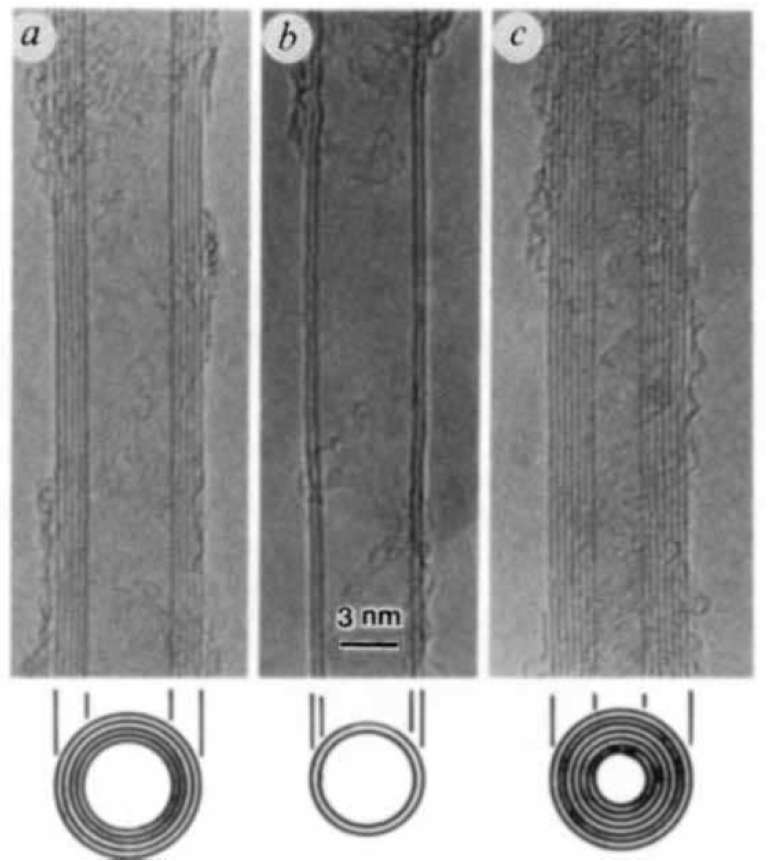
\includegraphics[width=.6\linewidth]{CNT/MWCNTiijima1991.png}  
  \caption{Nanotubos de carbono de pared múltiple descubiertos por Iijima en 1991, figura tomada de \cite{Iijima1991}.}
  \label{fig:iijima1991}
\end{subfigure}
\begin{subfigure}{.5\textwidth}
  \centering
  % include second image
  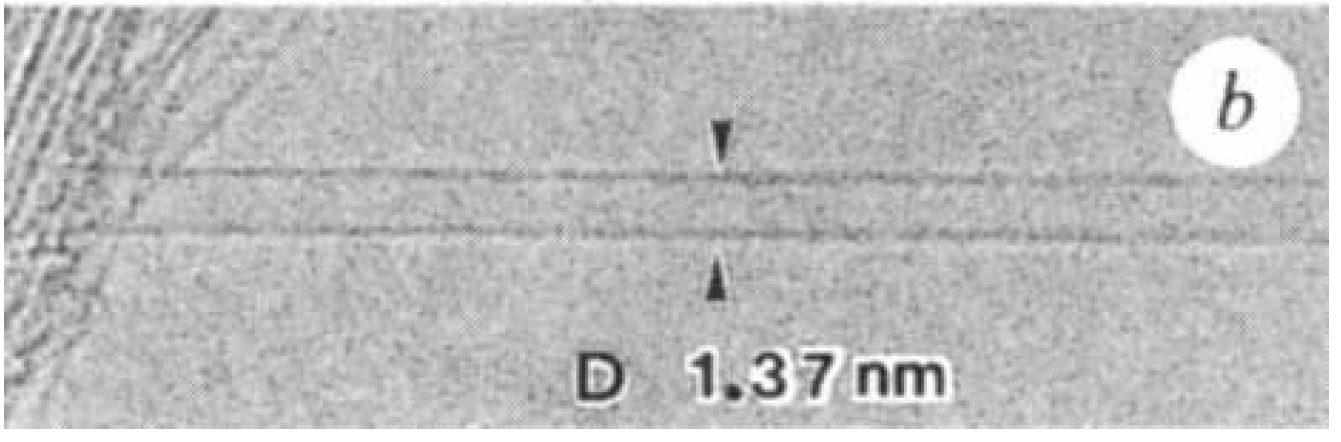
\includegraphics[width=.7\linewidth]{CNT/SWCNTiijima1993.png}  
  \caption{Nanotubo de carbono de pared simple descubierto por Iijima en 1993, figura tomada de \cite{Iijima1993}.}
  \label{fig:iijima1993}
\end{subfigure}
% \caption{Nanotubos presentados por Iijima en sus trabajos de 1991 y 1993 respectivamente.}
% \label{fig:IijimaCNTs}
\end{figure}

\newpage

Después de su descubrimiento se desarrolló una descripción teórica basada en su geometría para predecir propiedades físicas.

\subsection{Estructura de los nanotubos de carbono}\label{teoriaCNT}

En esta sección se presenta la descripción moderna de nanotubos de carbono y la predicción del tipo de nanotubo en función de sus propiedades eléctricas.\\

Un nanotubo de carbono es una sábana de arreglo hexagonal de carbonos enrollada alrededor de un eje, tiene la forma de un cilindro como en la figura \ref{fig:CNTejemplo}.\\

\begin{figure}[!h]
    \centering
    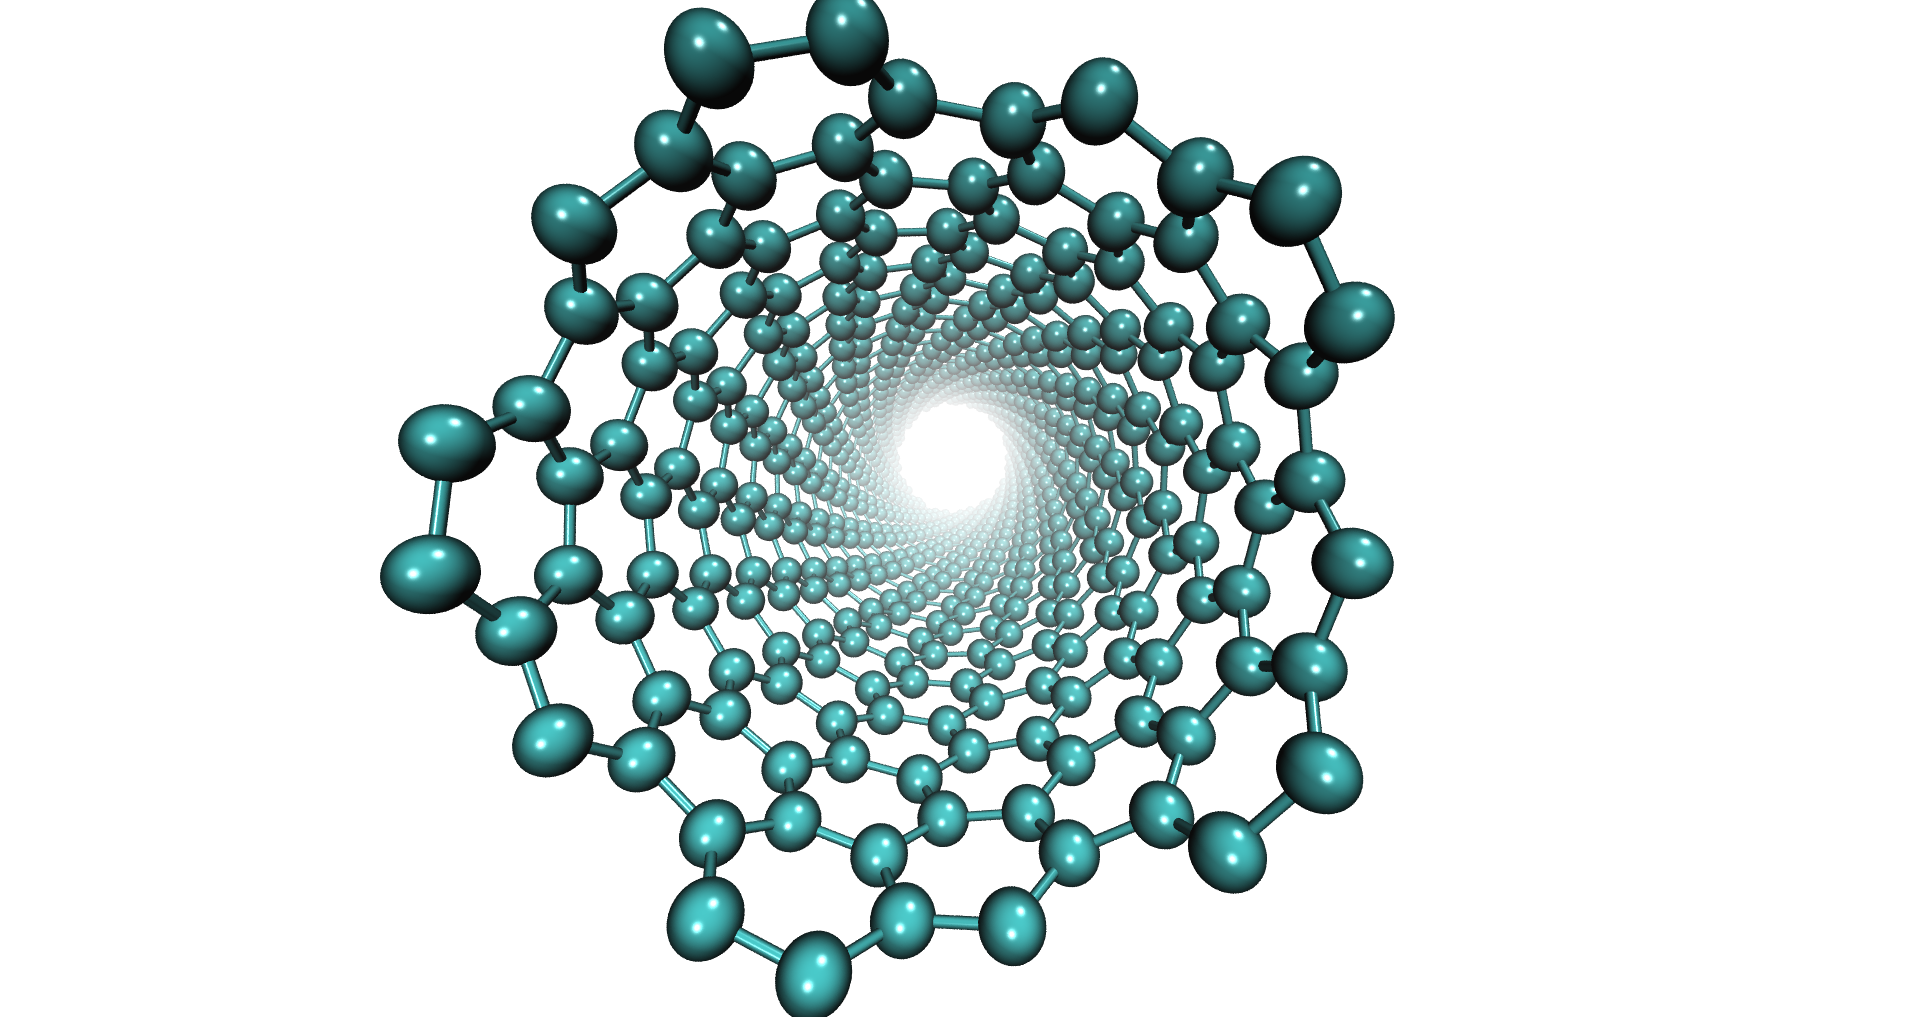
\includegraphics[width=.5\textwidth,keepaspectratio=true]{CNT/CNTejemplo.png}
    \caption{Nanotubo de carbono (5,10).}
    \label{fig:CNTejemplo}
\end{figure}

Para el cálculo y descripción de esta estructura, se presenta la tabla \ref{tab:carbono} donde se muestran los parámetros del carbono y del enlace carbono-carbono, así como el ángulo de enlace encontrado en el arreglo hexagonal.

\begin{table}[h!]
    \centering
    \begin{tabular}{ |p{4cm}|p{2cm}|  }
    \hline
    Parámetros  & Valor \\
    \hline
    longitud de enlace C-C   & 1.42 \AA \\
    \hline
    C-C-C($\theta$)   & 120 $^{\circ}$ \\
    \hline
    q (carga) & 0 e \\
    \hline
    m (masa)   & 12.0107 u \\
    \hline
    \end{tabular}
    \caption{Parámetros de enlace, ángulo de enlace, carga y masa de los carbonos en el arreglo hexagonal \cite{Melendez2016}.}
    \label{tab:carbono}
\end{table}

\newpage

\subsection{Geometría y notación (n,m)}

Los nanotubos de carbono en los textos científicos actuales se describen por un par de números enteros (n,m). Este describe completamente la estructura del nanotubo y ayuda en la predicción de sus propiedades físicas.\\

La geometría se puede describir usando los vectores $\mathbf{a_1}$ y $\mathbf{a_2}$, por convención los vectorres están arreglados como se muestra en las figura \ref{fig:CNT}.

\begin{figure}[!h]
\imagewidth=0.6\textwidth
\captionsetup[subfigure]{width=0.8\imagewidth,justification=raggedright}
\begin{subfigure}{.5\textwidth}
  \centering
  % include first image
  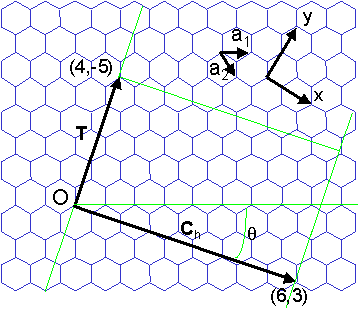
\includegraphics[width=.6\linewidth]{ChCNT.png}  
  \caption{Sábana de arreglo hexagonal donde se describen los ejes del plano $x,\ y$, los vectores $\mathbf{a_1}$ y $\mathbf{a_2}$; y el vector quiral de un nanotubo de carbono(6,3) junto con su vector de traslación T.}
  \label{fig:ChCNT}
\end{subfigure}
\begin{subfigure}{.5\textwidth}
  \centering
  % include second image
  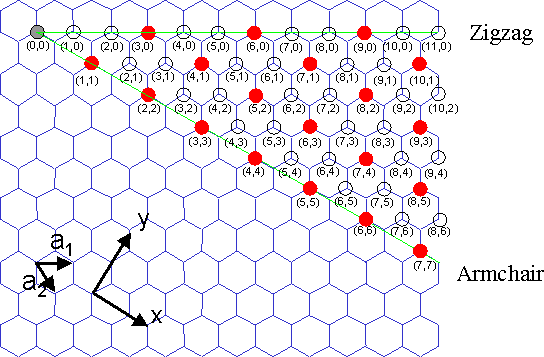
\includegraphics[width=.75\linewidth]{NT.png}  
  \caption{Los puntos rojos representan nanotubos metálicos y los círculos abiertos representan los semiconductores.}
  \label{fig:CNT}
\end{subfigure}
\caption{Quiralidad y simetría en nanotubos, figuras tomadas del sitio del Dr. Shigeo Maruyama consultado el 15 de febrero de 2020 \cite{ShigeoChiral}.}
\label{fig:GeoVectChir}
\end{figure}

El vector quiral $\mathbf{C_h}$ está descrito como en la ecuación (\ref{vectorquiral}).\\

\begin{equation} \label{vectorquiral}
    \mathbf{C_h} = n\mathbf{a_1} + m\mathbf{a_2}\quad n,m\in \mathbb{N}
\end{equation}

donde su magnitud es:

\begin{equation} \label{magnvectorquiral}
    \left|\mathbf{C_h}\right| = \sqrt{3}a_{cc}\sqrt{n^2+m^2+nm}
\end{equation}

la magnitud del vector quiral es el perímetro del nanotubo, así, el diámetro del nanotubo es:

\begin{equation} \label{diametroCNT}
    d_T = \left|\mathbf{C_h}\right|/\pi
\end{equation}

% El vector de traslación $\vec{T}$ es el vector más corto perpendicular a $C_h$ que empieza y termina en un punto del arreglo hexagonal:

% \begin{equation} \label{vectortraslacion}
%     \vec{T} = \left[\left(2m+n\right)\vec{a_1} - \left(2n+m\right)\vec{a_2}\right]/d_R
% \end{equation}

% \begin{itemize}
%     \item Vector de traslación: $\vec{T} = \left[\left(2m+n\right)\vec{a_1} - \left(2n+m\right)\vec{a_2}\right]/d_R$
%     \item Magnitud del vector de traslación: $\left|\vec{T}\right|=\sqrt{3}a_{cc}\frac{\left|C_h\right|}{d_R}$
% \end{itemize}

% donde:

% \begin{equation}\label{dR}
%     d_R =
%     \begin{cases} 
%     d,& \text{si } n-m \text{ no es múltiplo de } 3d\\
%     3d,& \text{si } n-m \text{ es múltiplo de } 3d
%     \end{cases}
% \end{equation}\\

Cuando $n-m/3$ es un entero los nanotubos son metálicos, en todos los demás casos el nanotubo es semiconductor \cite{Melendez2016}, esto puede observarse en la figura \ref{fig:CNT}.\\

También podemos separar en categorías por el patrón que se observa en la dirección del vector quiral. Cuando n=m, el nanotubo armchair se caracteriza por el patrón que se puede observar en la figura \ref{fig:armchair} en la dirección del vector quiral, este es siempre metálico; así en el caso $m=0$, el nanotubo zigzag se observa un patrón en zigzag como la figura \ref{fig:zigzag}; y en los demás casos el nanotubo se denomina quiral, un ejemplo es el de la figura \ref{fig:quiral}.

\begin{figure}[!hbt]
\begin{subfigure}{.5\textwidth}
  \centering
  % include first image
  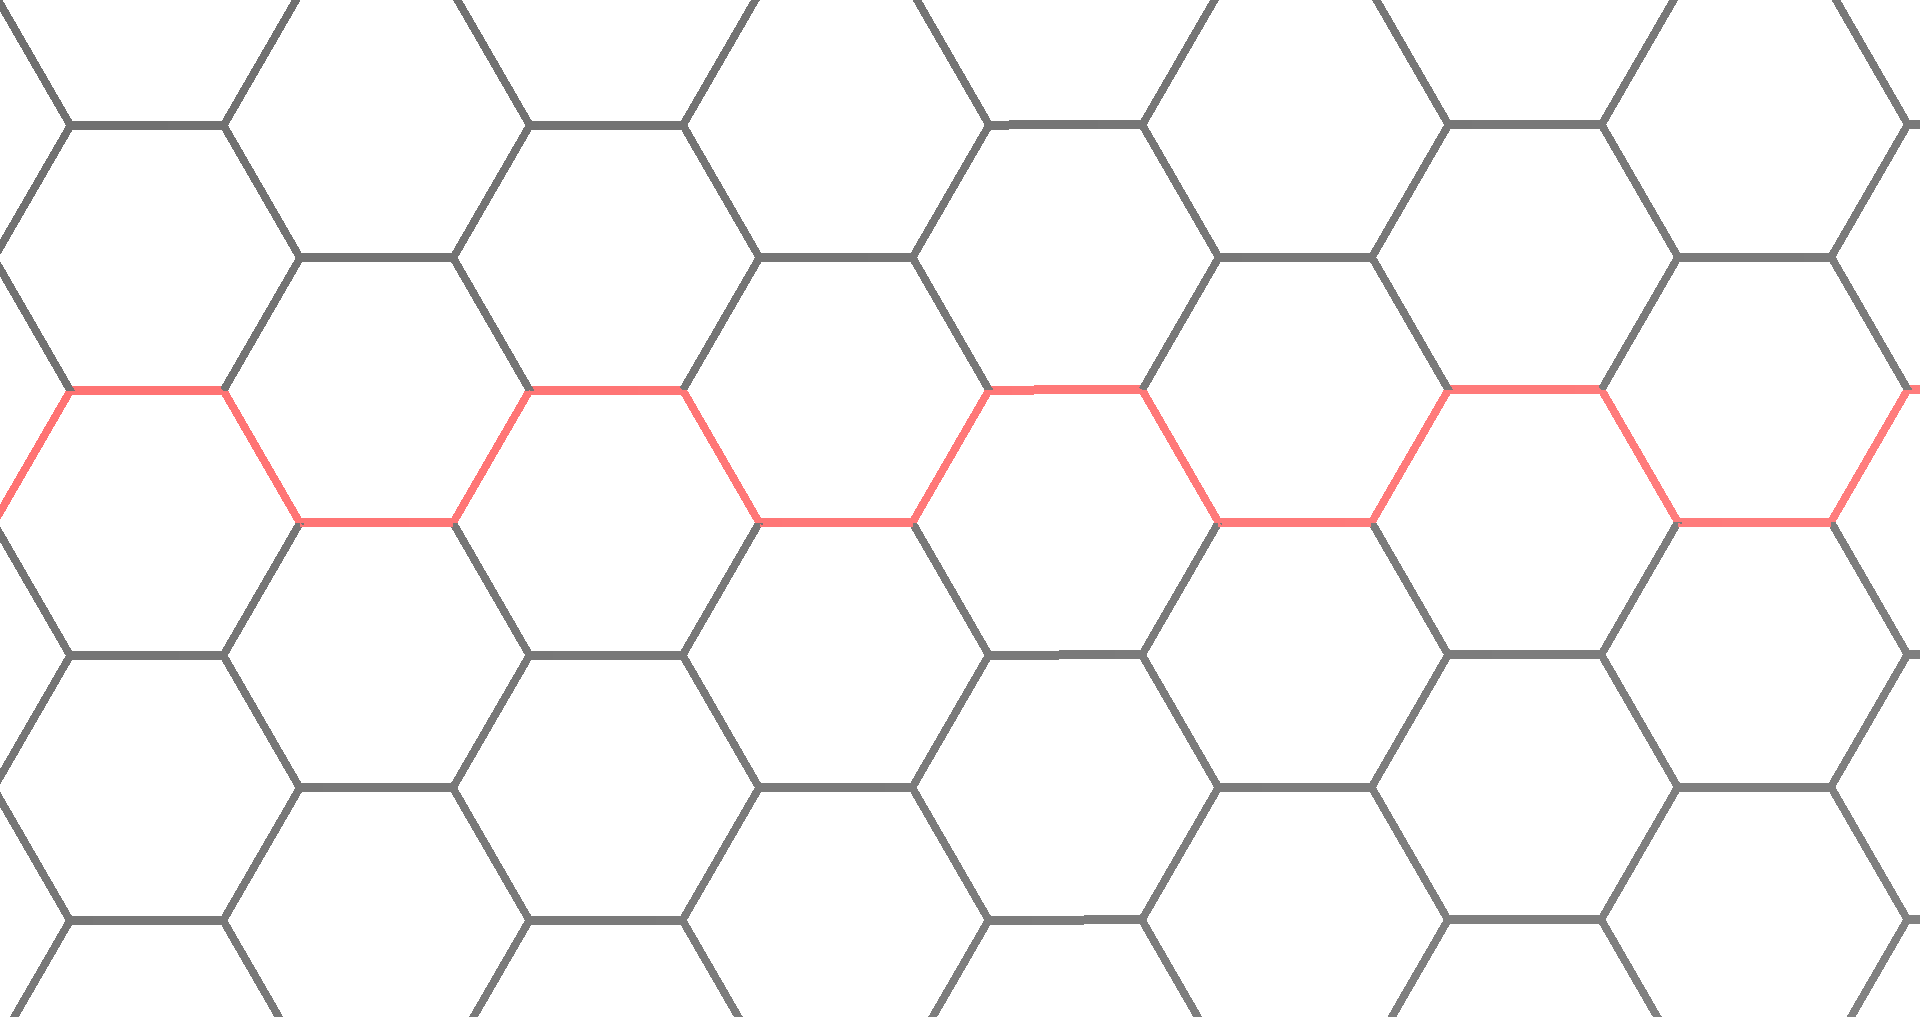
\includegraphics[width=.8\linewidth]{armchair.png}  
  \caption{Un SWCNT armchair desenrollado.}
  \label{fig:armchair}
\end{subfigure}
\begin{subfigure}{.5\textwidth}
  \centering
  % include second image
  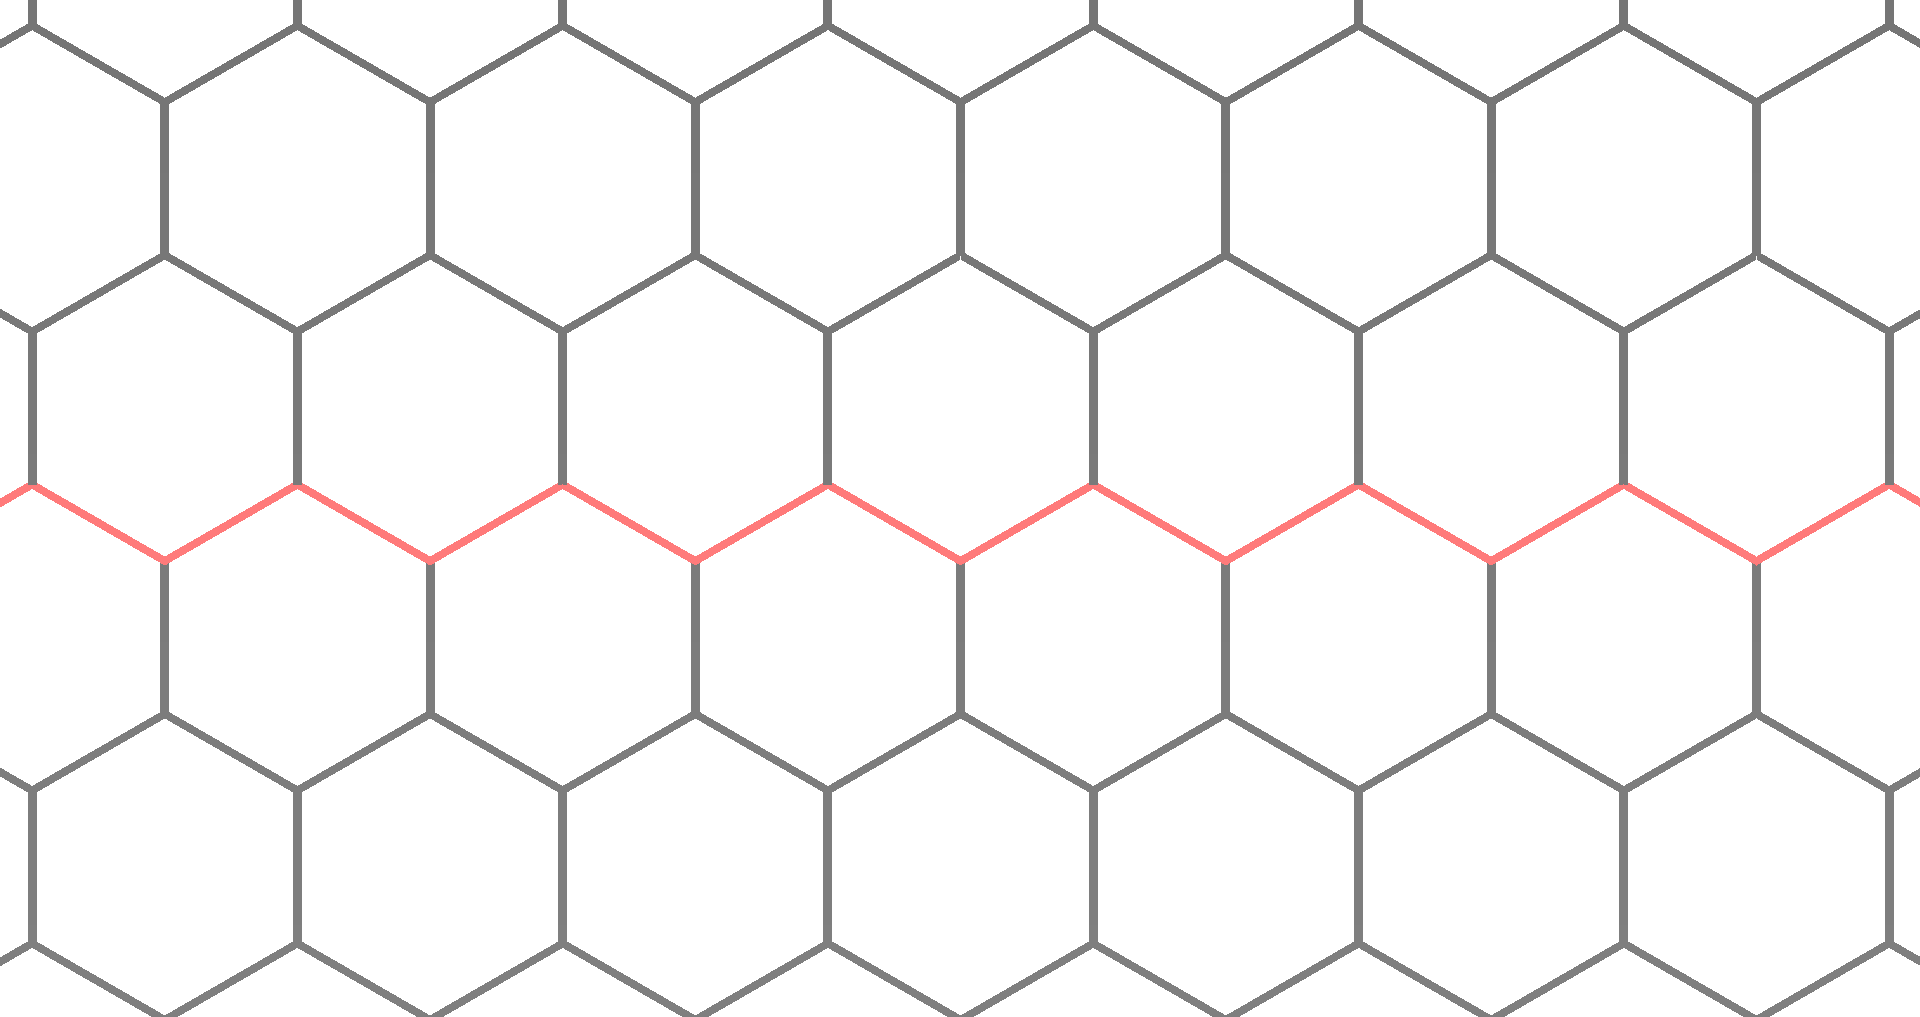
\includegraphics[width=.8\linewidth]{zigzag.png}  
  \caption{Un SWCNT zigzag desenrollado.}
  \label{fig:zigzag}
\end{subfigure}
\begin{subfigure}{1\textwidth}
  \centering
  % include second image
  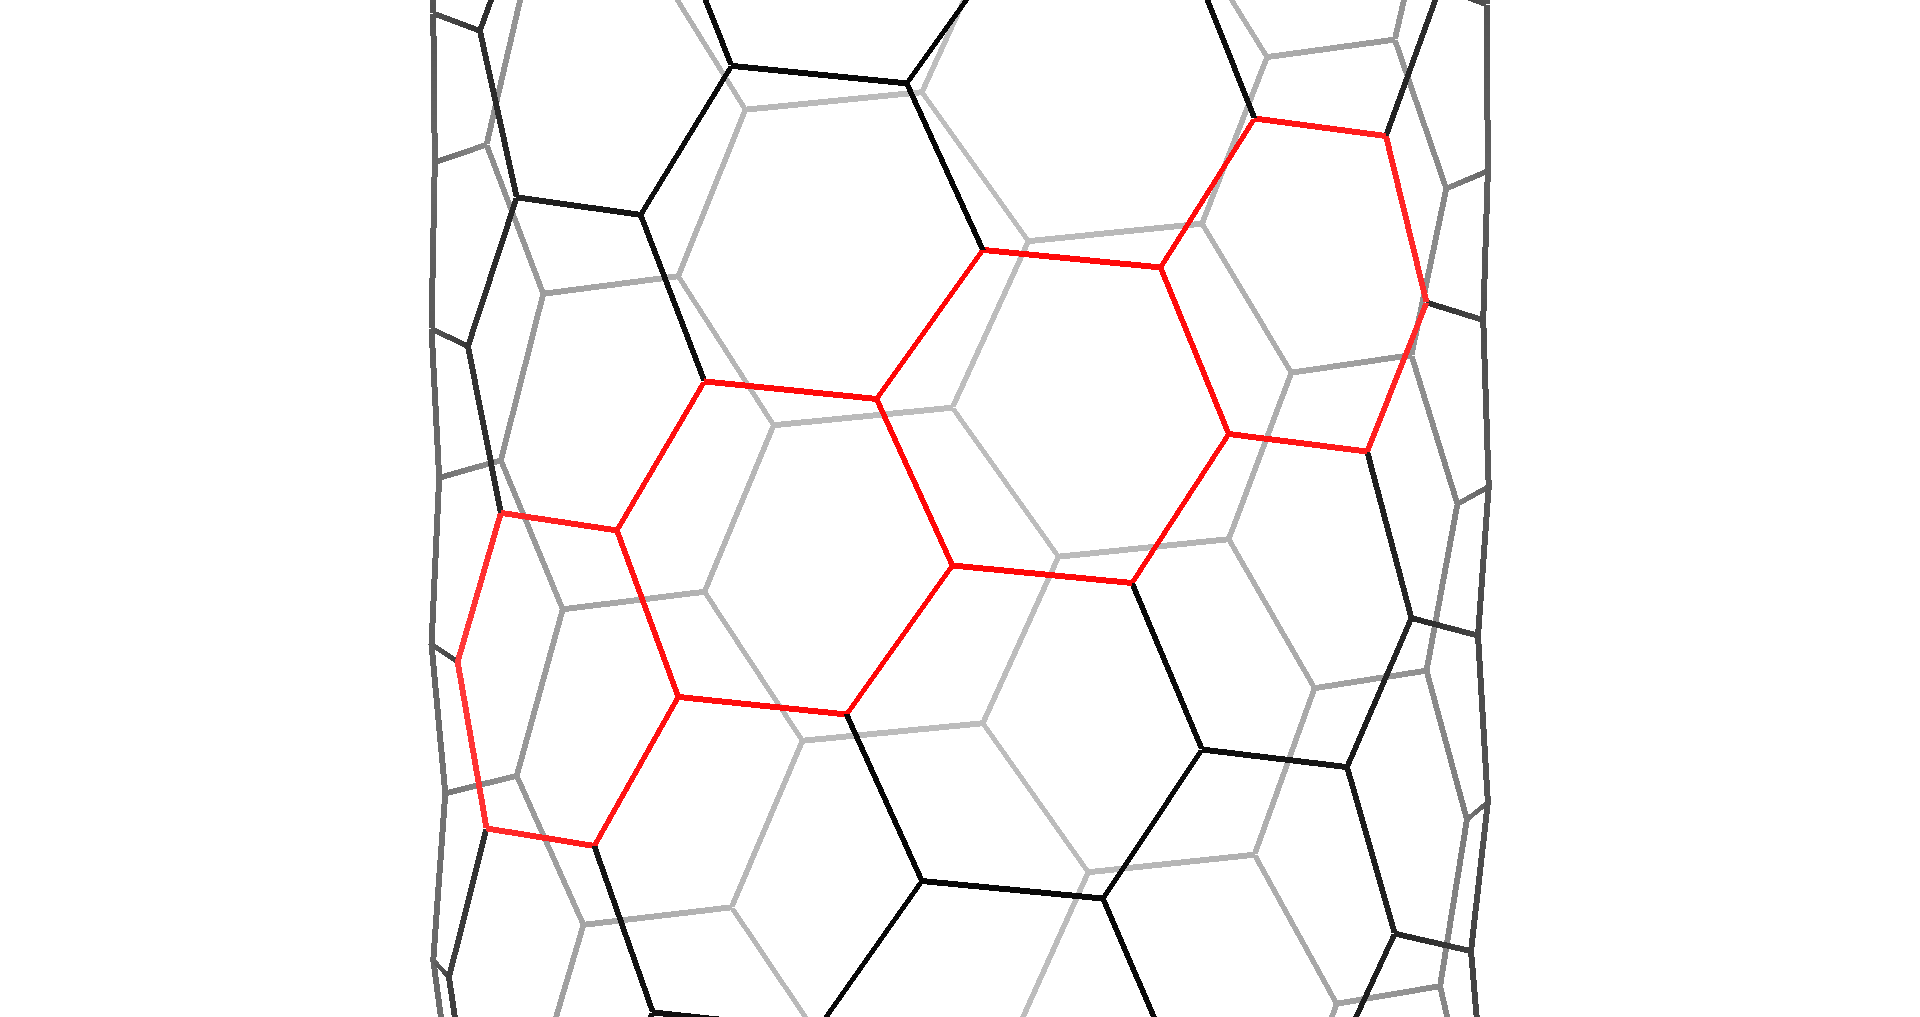
\includegraphics[width=.5\linewidth]{quiral.png}  
  \caption{Un SWCNT (7,5) quiral.}
  \label{fig:quiral}
\end{subfigure}
\caption{Los tres tipos de nanotubos de carbono.}
\label{fig:CNTsbygeometry}
\end{figure}

% \newpage

\subsection{Métodos de síntesis de nanotubos de carbono}

Se presentan a continuación los métodos mas importantes para la creación de nanotubos de carbono que se han desarrollado. Los métodos que se presentan varían en capacidad de creación, rendimiento y pureza.

\subsubsection{Método de descarga de arco}

En una cámara de descarga se usan como electrodos varillas de carbón y se llena con $\sim$500 torr de helio, adicionalmente para generar SWCNT se necesita de un catalizador como hierro, níquel o cobalto entre los electrodos. Este fue el método que uso Iijima en 1991 y 1993 para sintetizar por primera vez nanotubos de carbono. Lamentablemente este método genera muchas impurezas como se observa en la figura \ref{fig:arcmethod} y se presenta en este trabajo por razones históricas.

\begin{figure}[!h]
    \centering
    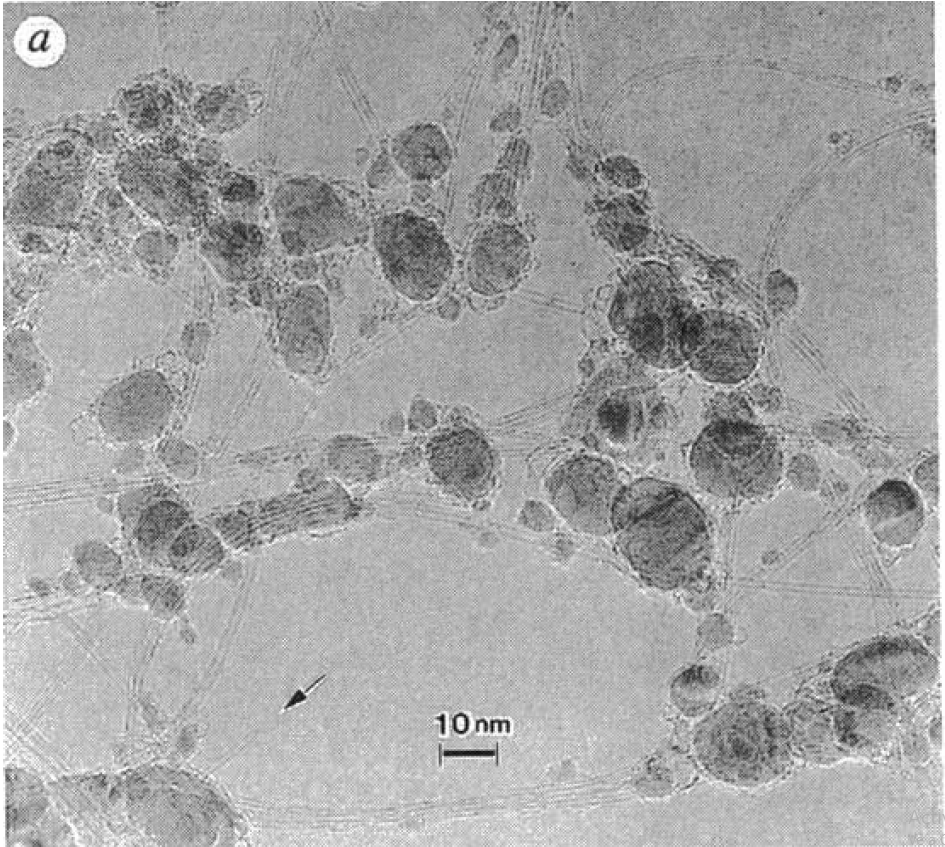
\includegraphics[width=.4\textwidth,keepaspectratio=true]{CNT/arcmethod.png}
    \caption{SWCNT con impurezas, figura tomada de \cite{Iijima1993}.}
    \label{fig:arcmethod}
\end{figure}

\newpage

\subsubsection{Ablación láser}

Este método usa un haz láser de alta potencia para evaporar un objetivo de grafito y crear las temperaturas necesarias para generar nanotubos de carbono. El objetivo de grafito al igual que en el método anterior usa un catalizador metálico. Se obtiene un alto rendimiento del 70\% al 90\% de conversión de grafito a SWCNT. La figura \ref{fig:ablationlasermethod} muestra el aparato usado en este método.

\begin{figure}[!h]
    \centering
    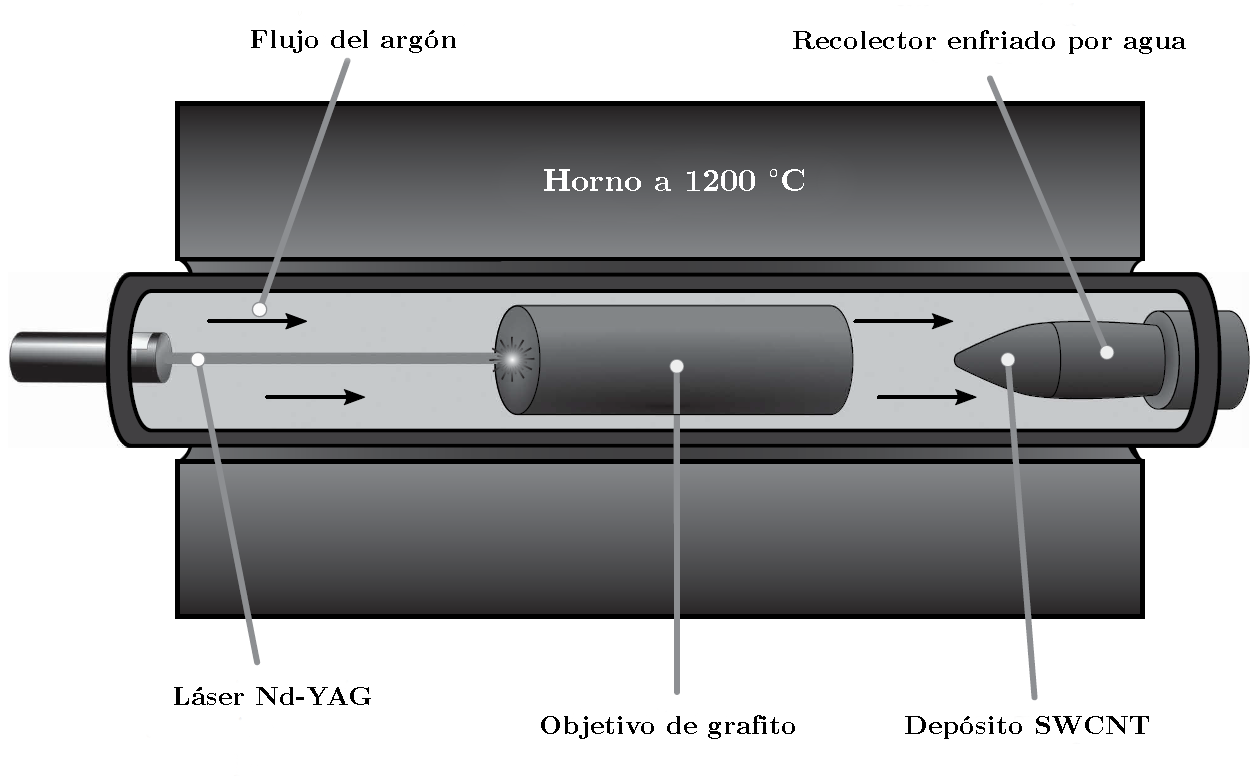
\includegraphics[width=.6\textwidth,keepaspectratio=true]{CNT/laserablationmethod.png}
    \caption{El objetivo de grafito está en una atmósfera de argón inerte a 1200$^{\circ}$C, el láser pulsado evapora el objetivo y los SWCNT son barridos a un colector afuera del horno por el flujo del argón. Figura adaptada de \cite{Melendez2016}.}
    \label{fig:ablationlasermethod}
\end{figure}

\subsubsection{Deposición de vapor químico catalítico (CCVD)}

Este método usa alguno de los gases metano, etano, etileno, acetileno como fuente de carbono, se introduce este en un horno a 600-900$^{\circ}$C junto con hidrógeno y argón, donde se genera una descomposición térmica de la fuente de carbono y crecen los nanotubos en un sustrato comúnmente de silicio que está en el horno como se muestra en la figura \ref{fig:ccvdmethod}. No obstante, los nanotubos de carbono de este método son de calidad pobre y la proporción de carbón que entra al horno y termina en un nanotubo es poca.

\begin{figure}[!h]
    \centering
    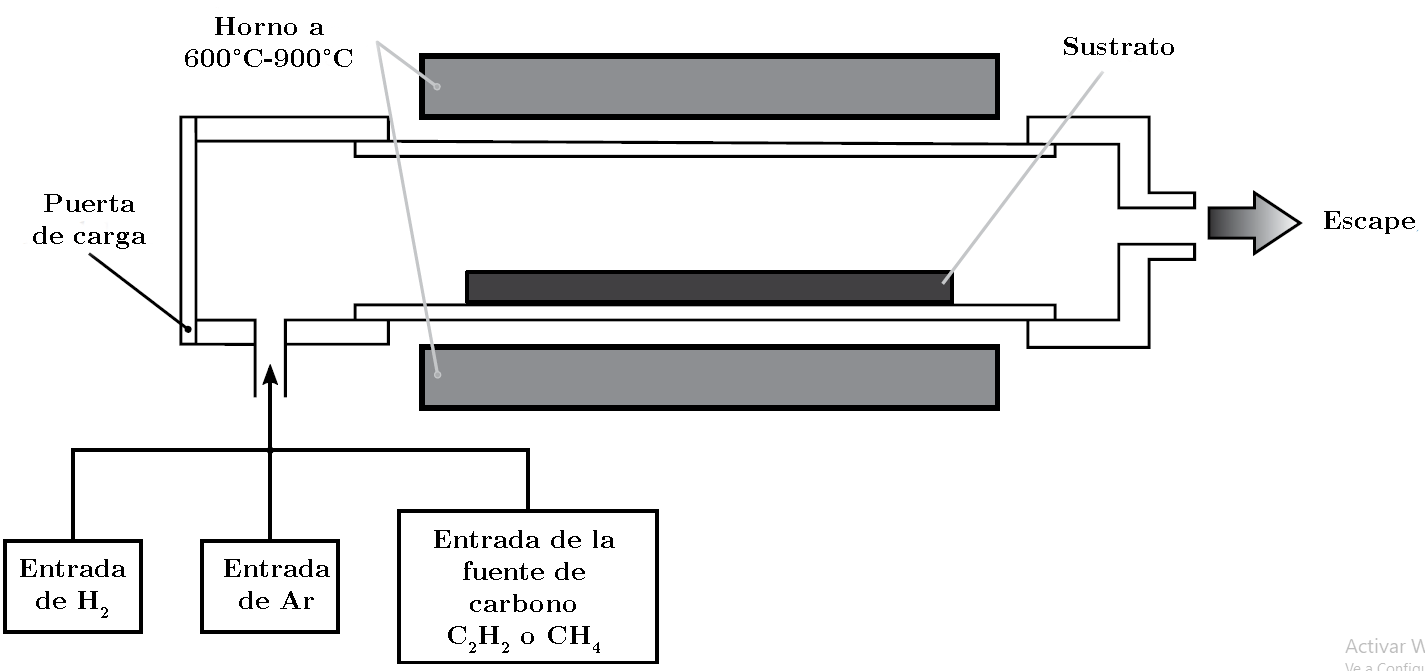
\includegraphics[width=.6\textwidth,keepaspectratio=true]{CNT/CCVD.png}
    \caption{Esquemático de un aparato  para crecimiento de nanotubos de carbono usando el método CCVD, figura adaptada de \cite{Melendez2016}.}
    \label{fig:ccvdmethod}
\end{figure}

\subsubsection{Deposición de vapor químico mejorada con plasma (PECVD)}

En el horno del método anterior, introducimos parcialmente calor en el horno y parcialmente con plasma sobre el sustrato. Este proceso ofrece dos ventajas sobre el anterior, reduce el costo de producción y mejora la calidad de los nanotubos al tener menos defectos.

\subsection{Funcionalización}

Los nanotubos de carbono obtenidos en los métodos presentados en la sección anterior tienen superficies hidrofóbicas, la funcionalización de los nanotubos de carbono es la solución a este problema. La funcionalización es el proceso de síntesis química donde los grupos funcionales deseados pueden ser introducidos a las paredes del nanotubo para aplicaciones o consumo humano. Hay dos métodos de funcionalización: covalente (formación de enlace químico) y enlace no covalente (fisisorción)\cite{KAUR2019}.

\subsubsection{Enlace covalente}

Hay varias reacciones covalentes para injertar moléculas basados en varias propiedades que pueden ser clasificados en reacciones ``injerto de'' e ``injerto a''. La modificación de enlace covalente mas usado es la oxidación de los nanotubos de carbono, para esta modificación se usan agentes oxidantes como ácido nítrico concentrado. En los nanotubos resultantes, se forman grupos de carboxil en los extremos y en los defectos de las paredes.

\subsubsection{Enlace no covalente}

Esta funcionalización es la más usada para nanotubos usados en la entrega de drogas al cuerpo. En contraste con la funcionalización anterior, se revisten los nanotubos con moléculas surfactantes anfifílicas o con polímeros. Este también preserva las propiedades físicas del nanotubo.


\subsection{Usos y aplicaciones}

Se han realizado múltiples investigaciones sobre el uso y las aplicaciones de los nanotubos de carbono por sus propiedades metálicas, semiconductoras y geométricas. Uno de los últimos avances en la fabricación de microprocesadores fue la creación del primer procesador hecho de transistores de nanotubos de carbono \cite{Hills2019} como se muestra en la figura \ref{fig:rv16xnano}, pensado por las limitaciones de tamaño y la poca eficiencia de energía eléctrica de los transistores de silicio.\\

\begin{figure}[!h]
    \centering
    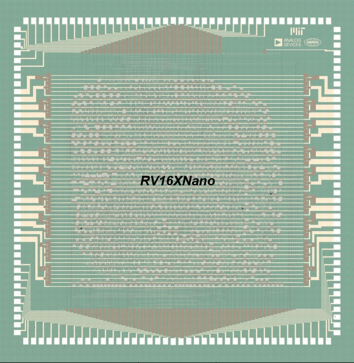
\includegraphics[width=.4\textwidth,keepaspectratio=true]{CNT/rv16x-nano.png}
    \caption{Microprocesador RV16X-nano hecho con transitores de nanotubos de carbono, figura tomada de \cite{Hills2019}.}
    \label{fig:rv16xnano}
\end{figure}

Otro ejemplo de aplicación reciente es en la industria automotriz, con la popularidad reciente de los coches eléctricos ha habido un interés por mejorar la capacidad y el tiempo de carga de las baterías, por ejemplo, BMW junto con la universidad de Hanyang mejoraron baterías de litio al incorporar nanotubos en el ánodo, lo que ha incrementando su densidad de energía y los ciclos de carga \cite{lee2016}.\\

% Los nanotubos de carbono se han vuelto fuertes candidatos en el campo de la ingeniería biomédica, biotecnología y nanotecnología farmacéutica. Han habido varios estudios y aplicaciones, dentro de los que destacan son: imageneología biomédica en rayos X, terapia en infecciones, regeneración de tejidos, tratamiento de cancer entre otros \cite{KAUR2019}.

También hay múltiples tratamientos de remoción de contaminantes en agua usando nanotubos de carbono, por ejemplo: el triclosán e ibuprofeno han sido exitosamente removidos por adsorción de medios acuosos usando SWCNT, igual ha sido removido plomo(II) usando MWCNT recubierto de óxido y muchos otros.\\

En la figura \ref{fig:remocioncontCNT} se relacionan algunos procesos de funcionalización de CNT con aplicaciones en remoción o disminución de contaminantes en agua.

% los contaminantes emergentes(son químicos sintéticos o naturales y microorganismos que no son monitoreados comunmente pero que tienen un potencial contaminante en el ambiente)

\begin{figure}[!h]
    \centering
    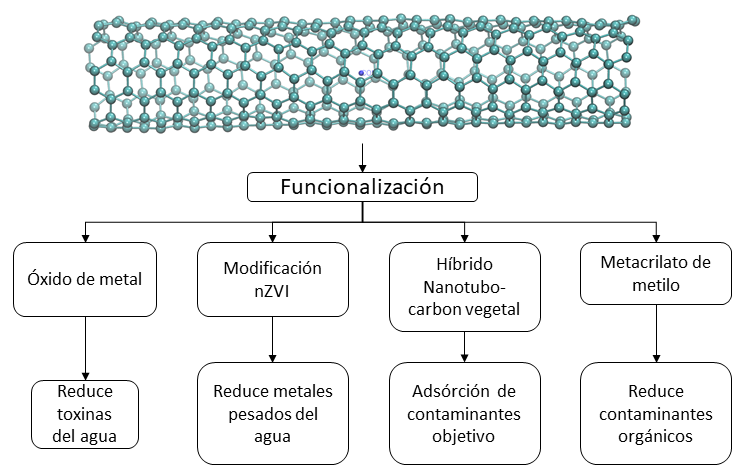
\includegraphics[width=.7\textwidth,keepaspectratio=true]{CNT/esquemafuncCNT.png}
    \caption{Diagrama esquemático representando alguno procesos de funcionalización de CNT para remoción de contaminantes en agua y aguas residuales. Figura adaptada de \cite{SARKAR2018}.}
    \label{fig:remocioncontCNT}
\end{figure}
\newpage

\section{Herbicida 2,4-D}

El ácido 2,4-diclorofenoxiacético o 2,4-D es un herbicida tóxico y contaminante ambiental ampliamente usado en tierra y agua. Hay nueve formas de 2,4-D que pueden ser usados como herbicida y es regularmente vendido como polvo o en su forma líquida. Tiene un peso molecular de 221.03 g/mol, con una densidad relativa al agua entre 0.7-0.8 y con fórmula molecular C8H6Cl2O3 \cite{24dpubchem}.

\begin{figure}[!h]
    \centering
    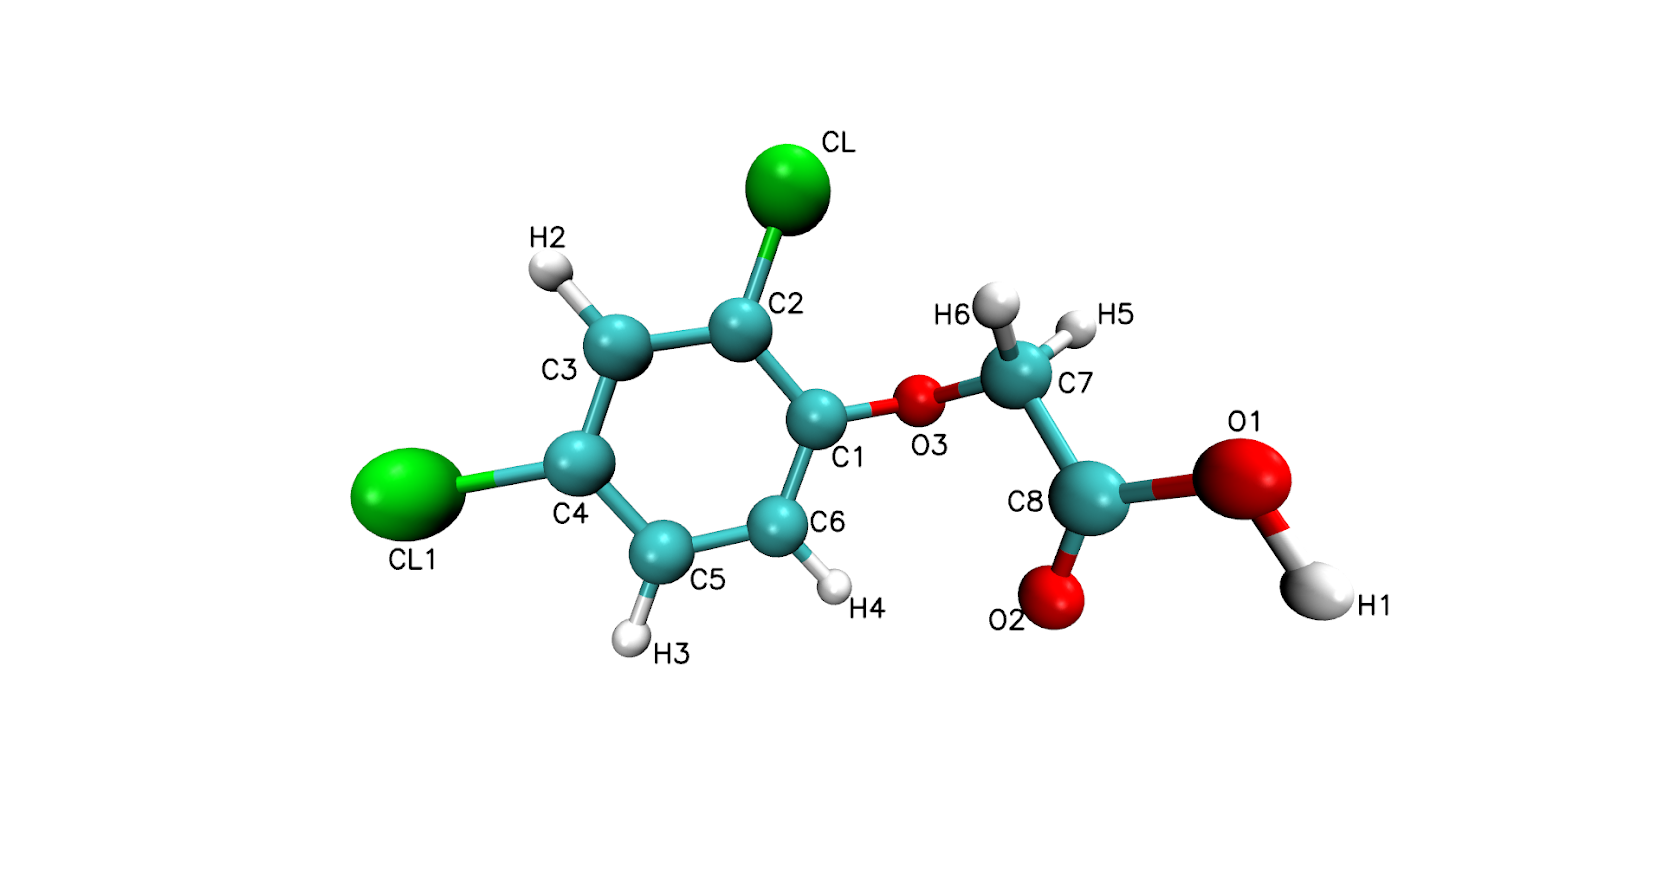
\includegraphics[width=.7\textwidth,keepaspectratio=true]{24d/24d_label.png}
    \caption{Modelo de molécula 2,4-D usado en el trabajo.}
    \label{fig:24detiquetas}
\end{figure}

La exposición prolongada de este herbicida en el humano genera múltiples enfermedades como asma, hipotiroidismo, complicaciones del embarazo, infertilidad en hombres, entre otros \cite{24dpubchem}.

\section{Agua}

El agua es una molécula importante para la vida y elemental para la supervivencia de las especies. Hay múltiples modelos de agua, para este trabajo se usó el modelo SPC/E. Este tiene cargas situadas en los tres átomos y la interacción Lennard-Jones con otras moléculas está situada en el oxígeno. La figura (\ref{fig:SPCE}) es una visualización de la molécula y la tabla (\ref{SPCEpar}) son los parámetros del modelo.

\begin{figure}[!h]
    \centering
    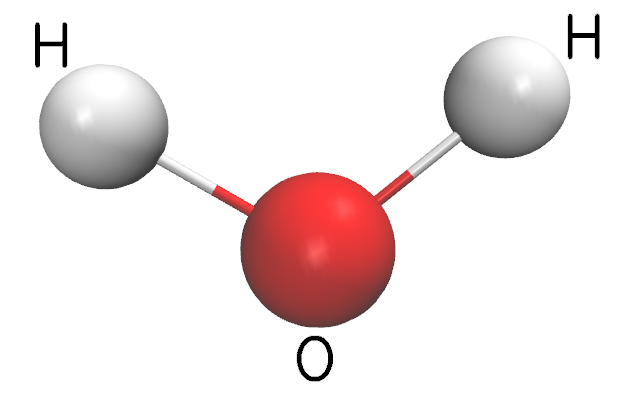
\includegraphics[width=.3\textwidth,keepaspectratio=true]{SPCE.png}
    \caption{Figura representativa de una molécula de agua}
    \label{fig:SPCE}
\end{figure}

\begin{table}[h!]
    \centering

    \begin{tabular}{ |p{2cm}|p{3cm}|  }
    \hline
    Parámetro  & Valor \\
    \hline
    $\sigma$  & 3.166 \AA \\
    $\epsilon$& 0.650 KJ $mol^{-1}$ \\
    $r_{OH}$  & 1.000 \AA \\
    $\angle_{HOH}$&109.47 deg \\
    $q_{O}$   & -0.8476 e \\
    $q_{H}$   & 0.4238 e \\
    \hline
    \end{tabular}
    \caption{Parámetros del modelo SPCE}
    \label{SPCEpar}
\end{table}


\chapter{Mecánica estadística clásica}\label{chap:mecanica_estadistica}

En este capítulo presentamos las bases teóricas de la mecánica estadística clásica como marco de estudio microscópico de sistemas macroscópicos.

\section{Fundamentos teóricos}

La mecánica estadística estudia a los sistemas macroscópicos termodinámicos a partir de leyes dinámicas microscópicas. Supongamos un sistema caracterizado por las variables termodinámicas $A_1$, $A_2$..., como por ejemplo, energía, volumen, presión, entre otras; y este macroestado queda determinado por un conjunto de valores de sus variables termodinámicas denominado $\alpha$=$B_1(\mathbf{r}, t)$, $B_2(\mathbf{r}, t)$... Un estado macroscópico del sistema (o {\it macroestado} denotado como $(A_1, A_2...;\alpha)$) es análogo a una observación macroscópica dadas por sus variables termodinámicas, en cambio, un estado microscópico (o microestado) está definido por coordenadas $q$ y momentos $p$ de las partículas que forman el sistema y que son consistentes con el macroestado $(A_1, A_2...;\alpha)$.\\

Sin embargo, no todos los macroestados del sistema corresponden al sistema en equilibrio, aquellos que pertenecen al sistema en equilibrio se les denota como $(A_1, A_2...;\alpha^{*})$ o $(A_1, A_2...)$. El total de microestados asociados a un macroestado de equilibrio se denota por $\Omega(A_1, A_2...)$.\\

% En el siguiente ejemplo tenemos una caja sujeta a movimientos aleatorios con partículas de diferentes colores que empiezan en un macroestado de no equilibrio y rapidamente tienden al equilibrio como en la siguientes figuras bla bla.\\

Adicionalmente, es un hecho experimental una vez que alcanza que un sistema aislado el equilibrio se mantiene en ese macroestado, esto permite concluir que el número de microestados correspondientes a $(A_1, A_2...)$ es mucho mayor que los microestados correspondientes a otros macroestados de no equilibrio.\\

% De acuerdo con la mecánica clásica, la dinámica de un sistema de partículas se resuelve solucionando las ecuaciones de movimiento de las partículas.
% Sin embargo, cuando las partículas interactúan entre sí, resolver la dinámica del sistema por cualquiera de los métodos en dinámica (Newton, Lagrange o Hamilton) sería un cálculo básicamente imposible o poco práctico. A pesar de ello el marco conceptual es extremadamente útil y por ello describiremos enseguida los postulados de la mecánica estadística de equilibrio y el concepto de ensamble.\\

Dos postulados fundamentales de la física estadística crean una relación entre las escalas microscópica y macroscópica \cite{Huang_1987}\cite{tuckerman2010}.\\

\begin{itemize}
    \item Postulado de equiprobabilidad: Cuando un sistema macroscópico está en equilibrio termodinámico, sus microestados asociados son igualmente probables.
    
    \item Postulado de la entropía: En un sistema en equilibrio, su entropía $S$ está dada por:
    \begin{equation}\label{postulado_entropia_boltx}
        S=k_{B}ln(\Omega(A_1, A_2...))
    \end{equation}
    con $k_B$ la consstante de Boltzmann.
\end{itemize}

Como se puede observar de la ecuación (\ref{postulado_entropia_boltx}), la entropía vincula de manera directa el comportamiento microscópico con un variable termodinámica, que en este caso es la entropía, la cual caracteriza el estado de equilibrio del sistema\\

Sin embargo, para describir estadísticamente a los sistemas termodinámicos aún nos falta una herramienta importante que se describe a continuación.

\section{Ensambles}

Un ensamble es una colección hipotética de $\mathcal{N}$ réplicas del sistema descritas por el mismo conjunto de interacciones microscópicas y que comparten un conjunto de propiedades macroscópicas como energía, volumen, número de partículas, entre otras \cite{tuckerman2010}. Como se verá a continuación en las ecuaciones (\ref{gibbspostulate}) y (\ref{ergodichip}) junto con los dos postulados anteriores, los ensambles son herramientas esenciales para el estudio de sistemas termodinámicos usando la mecánica estadística clásica.\\

% Los ensambles pueden ser definidos dependiendo de las situaciones termodinámicas que se impongan al sistema, y dependiendo de \textcolor{yellow}{estos} se pueden extraer propiedades estáticas macroscópicas como la energía, temperatura, presión, etc. Los ensambles que cumplen esta propiedad estática aun cuando el sistema se encuentra evolucionando en el tiempo son llamados \textit{Ensambles de equilibrio}.\\
En teoría de ensambles todas las observables macroscópicas del sistema están relacionadas a una función microscópica.\\

Se puede calcular el promedio temporal de una variable dinámica $A$ a través de

\begin{equation} \label{promediotemp}
    \langle A\rangle_{tiempo} = \lim_{t\to\infty}\frac{1}{t}\int_0^t A(t)dt
\end{equation}\\
en el intervalo de tiempo de 0 a $t$,
o por un promedio de ensamble asociado a probabilidades \cite{tuckerman2010}. \\
\begin{equation} \label{promedioequprob}
    \langle A\rangle_{ensamble} =\sum_r A_r P_r,
\end{equation}\\
con $P_r$ la probabilidad del r-ésimo microestado y $A_r$ el valor de $A$ en el r-ésimo microestado.\\

Las ecuaciones (\ref{promediotemp}) y (\ref{promedioequprob}) se encuentran directamente relacionados por dos postulados importantes \cite{mcquarrie1976}:

\begin{itemize}
    \item Postulado de Gibbs: El promedio de una propiedad mecánica (variable dinámica) corresponde a la propiedad termodinámica paralela.\\
    
    \begin{equation} \label{gibbspostulate}
        A \Longleftrightarrow \left \langle A \right \rangle
    \end{equation}
    
    \item Hipótesis ergódica: Medir un sistema para N instantes en el tiempo tiene las mismas propiedades estadísticas que medir N sistemas arbitrarios al mismo tiempo de un ensamble:
    \begin{equation} \label{ergodichip}
        \left \langle A \right \rangle_{tiempo} \Longleftrightarrow \left \langle A \right \rangle_{ensamble}.
    \end{equation}
\end{itemize}

El postulado de Gibbs relaciona una propiedad termodinámica a un promedio de un propiedad dinámica del sistema, esto es, cada variable termodinámica del sistema se calcula con el promedio de alguna propiedad mecánica microscópica. La hipótesis ergódica será importante en el siguiente capítulo por la relación que genera entre la mecánica estadística y la dinámica molecular.\\

Gracias a estos ensambles podemos describir sistemas termodinámicos con características diferentes. En esta tesis que representan sistemas reales se usaron dos ensambles de los cuatro ejemplos mostrados en la tabla \ref{tiposEnsamble},

\begin{table}[h!]
    \centering
    \begin{tabular}{ |p{3cm}||p{4cm}|  }
    \hline
    Cantidades fijas   & Ensambles \\
    \hline
    NVE   & Microcanónico \\
    NVT   & Canónico \\
    $\mu$VT& Gran Canónico \\
    NPT   & Isotérmico-Isobárico \\
    \hline
    \end{tabular}
    \caption{Ensambles comúnmente usados para describir sistemas termodinámicos.}
    \label{tiposEnsamble}
\end{table}

\noindent donde N es el número de partículas, V el volumen, E la energía interna, P la presión, $\mu$ el potencial químico y T la temperatura.

\subsection{Ensamble canónico NVT}

El ensamble canónico está formado por $\mathcal{N}$ copias de un sistema en equilibrio, contiene N partículas indistinguibles a temperatura T y volumen V. Los $\mathcal{N}$ sistemas del ensamble están en contacto entre si mediante paredes diatérmicas sólidas es decir, para cada sistema en este ensamble, el resto es su fuente de calor. El esquema del ensamble se muestra en la figura \ref{fig:CanonicEns}.\\

\begin{figure}[!h]
    \centering
    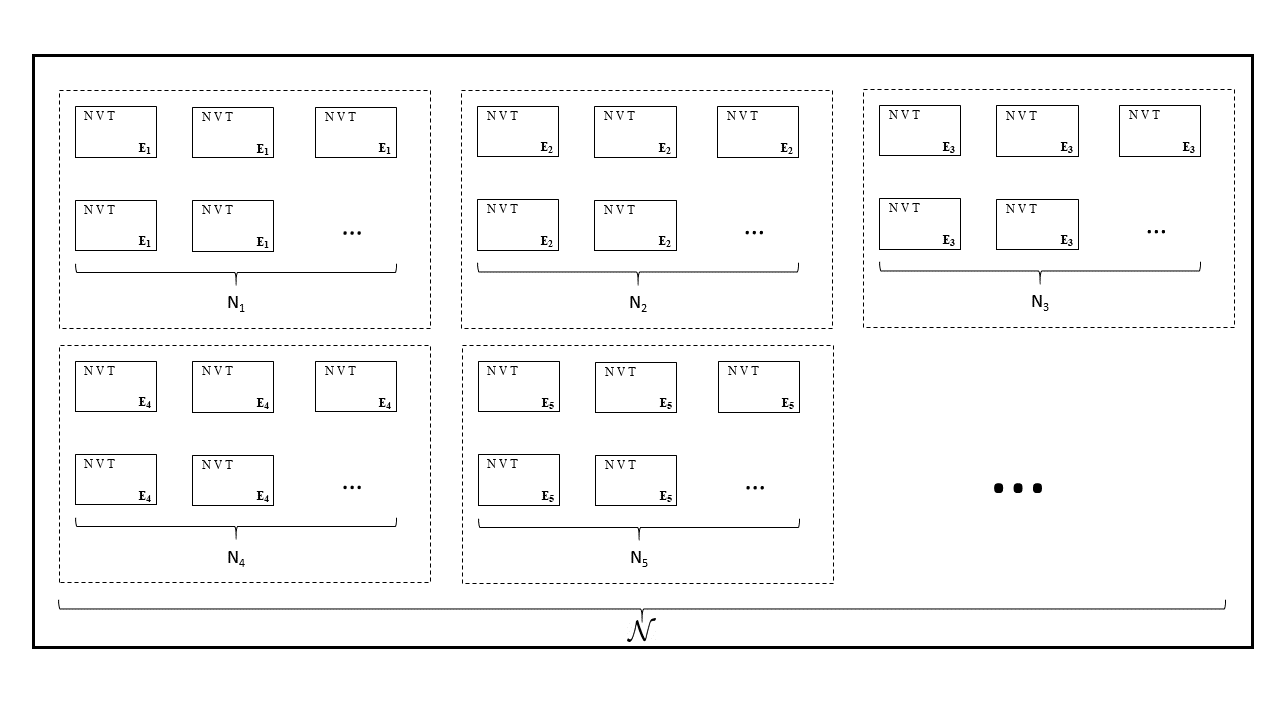
\includegraphics[width=1\textwidth,keepaspectratio=true]{StatMech/nvtensemble.png}
    \caption{Representación del ensamble canónico NVT. Cada sistema está en contacto con otro transfiriendo calor, los recuadros se usan para representar el conteo de degeneración de la energía.}
    \label{fig:CanonicEns}
\end{figure}

\newpage

Los sistemas del ensamble se encuentran en algunos de los $E_r$ niveles de energía, estos a su vez toman y ceden energía con su alrededor, es decir, los otros sistemas. Puede haber degeneración en algunos sistemas (sistemas diferentes pueden tener el mismo nivel de energía).\\

De acuerdo a lo anterior, tenemos:\\
\begin{center}
    $N_1$ sistemas con energía $E_1$\\
    $N_2$ sistemas con energía $E_2$\\
    ...\\
    $N_r$ sistemas con energía $E_r$\\
    ...\\
\end{center}

El total de sistemas es la suma de todos los $N_r$ sistemas.

\begin{equation} \label{conteoprob}
    \mathcal{N} = \sum_r N_r \\
\end{equation}

y

\begin{equation} \label{restrprob}
    1 = \sum_r P_r \\
\end{equation}

con $P_r = \frac{N_r}{\mathcal{N}}$ la probabilidad normalizada.\\

Por el postulado de Gibbs, el promedio de la energía de los sistemas es la energía del sistema.

\begin{equation} \label{energiaprob}
    U = \langle E\rangle = \sum_r P_r E_r.
\end{equation}

La combinación de microestados que se pueden formar son el número de microestados correspondientes que puede tomar el sistema, \\

\begin{equation} \label{ditrbmicro}
    \Omega = \frac{\mathcal{N}!}{\prod_r N_r!}.
\end{equation}\\

Sustituyendo la ecuación (\ref{ditrbmicro}) en (\ref{postulado_entropia_boltx}) se encuentra,

\begin{equation}  \label{entropiaboltz}
    S = k_{B}ln\left(\frac{\mathcal{N}!}{\prod_r N_r!}\right)
\end{equation}\\

\noindent y de acuerdo con la fórmula de Stirling, $lnN!=NlnN-N$, la ecuación (\ref{entropiaboltz}) se reduce a

\begin{equation}  \label{entropiaboltzstirling}
    S = -k_{B}\mathcal{N}\sum_r P_rln(P_r).
\end{equation}\\

Aplicando el método de los multiplicadores de Lagrange se halla lo siguiente \cite{greiner1995}:

\begin{equation} \label{probcan}
    P_r = \frac{e^{-\beta E_r}}{\mathcal{Z}}
\end{equation}
\noindent donde $\mathcal{Z} = \sum_r e^{-\beta E_r}$ es la función de partición canónica, con $\beta=\frac{1}{k_{B}T}$.\\

El potencial termodinámico del ensamble canónico es la energía libre de Helmholtz:

\begin{equation} \label{potHelm}
    F(N,V,T)=-k_{B}Tln(\mathcal{Z}).
\end{equation}

Las propiedades termodinámicas se obtienen de la función de partición canónica como se muestra en las ecuaciones (\ref{energcan}) y (\ref{ecestacan}).

\begin{equation} \label{energcan}
    U=k_{B}T^2\left( \frac{\partial ln(\mathcal{Z})}{\partial T} \right)_{N,V}
\end{equation}  

\begin{equation} \label{ecestacan}
    P=k_{B}T\left( \frac{\partial ln(\mathcal{Z})}{\partial V} \right)_{N,T}
\end{equation}

La entropía del sistema es \cite{mandl1988statistical}:

\begin{equation} \label{entrnvt}
    S = k_{B}\beta U + k_{B}ln(\mathcal{Z}).
\end{equation}

\subsection{Ensamble isobárico-isotérmico NPT}

El ensamble NPT está formado por $\mathcal{N}$ copias de un sistema en equilibrio con N partículas indistinguibles  a temperatura T y está acoplado a un pistón isotrópico que se comprime o expande en respuesta a fluctuaciones instantáneas de la presión interna (fuente de volumen). Los $\mathcal{N}$ sistemas de este ensamble están en contacto entre si por paredes diatérmicas y flexibles, es decir, para cada sistema en este ensamble, el resto es su fuente de calor y volumen como se muestra en la figura \ref{fig:NPTEns}.\\

Este ensamble es importante porque los datos experimentales de propiedades en fase condensada se encuentran a condiciones de presión y temperatura constante.\\

\begin{figure}[!h]
    \centering
    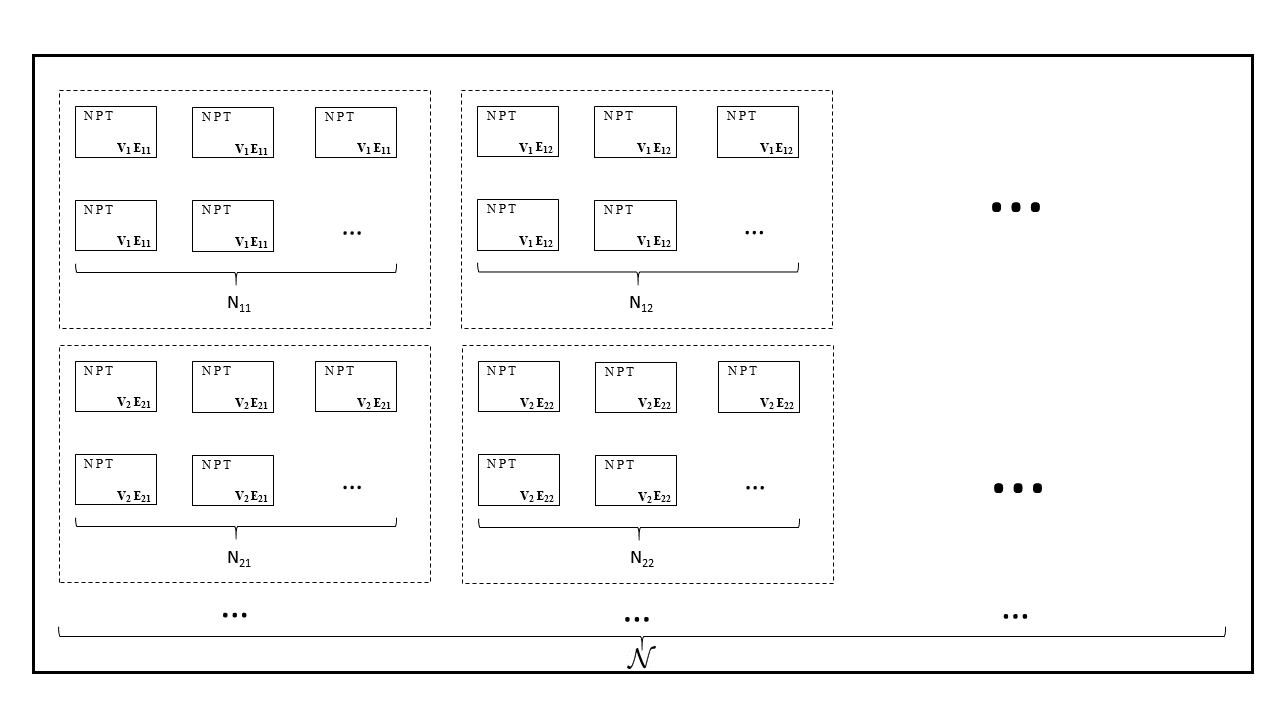
\includegraphics[width=1\textwidth,keepaspectratio=true]{StatMech/nptensemblefig.png}
    \caption{Representación del ensamble canónico NPT. Cada sistema está en contacto con otro transfiriendo calor y expandiéndose, los recuadros se usan para representar el conteo de degeneración de la energía.}
    \label{fig:NPTEns}
\end{figure}

Tenemos en este sistema lo siguiente:\\

\begin{center}
    $N_{1n}$ sistemas con energía $E_{1n}$ y volumen $V_1$\\
    $N_{2n}$ sistemas con energía $E_{2n}$ y volumen $V_2$\\
    ...\\
    $N_{rn}$ sistemas con energía $E_{rn}$ y volumen $V_r$\\
    ...\\
\end{center}

El total de los sistemas es la suma de todos los $N_{rn}$ sistemas.

\begin{equation} \label{conteoprobNPT}
    \mathcal{N} = \sum_{rn} N_{rn} \\
\end{equation}

entonces,

\begin{equation} \label{restrprobNPT}
    1 = \sum_{rn} P_{rn} \\
\end{equation}

con $P_{rn} = \frac{N_{rn}}{\mathcal{N}}$ la probabilidad normalizada.\\

Por el postulado de Gibbs, el promedio de la energía de las réplicas es la energía del sistema y el promedio del volumen de las réplicas es el volumen del sistema.

\begin{equation} \label{energiaprobNPT}
    U = \langle E\rangle = \sum_{rn} P_{rn} E_{rn},
\end{equation}

\begin{equation} \label{volprobNPT}
    V = \langle V\rangle = \sum_{rn} P_{rn} V_r.
\end{equation}

La combinación de microestados que se pueden formar son el número de microestados correspondientes que puede tomar el sistema, el cual es:\\

\begin{equation} \label{distribucionmultnom}
    \Omega = \frac{\mathcal{N}!}{\prod_{rn} N_{rn}!}.
\end{equation}\\

Sustituyendo la ecuación (\ref{distribucionmultnom}) en (\ref{postulado_entropia_boltx}) se encuentra,

\begin{equation}  \label{entropiaboltzNPT}
    S = k_{B}ln\left(\frac{\mathcal{N}!}{\prod_{rn} N_{rn}!}\right) 
\end{equation}\\

y de acuerdo con la fórmula de Stirling, $lnN!=NlnN-N$, la ecuación (\ref{entropiaboltzNPT}) se escribe como

\begin{equation}  \label{entropiaboltzNPTstirling}
    S =  -k_{B}\mathcal{N}\sum_{rn} P_{rn} ln(P_{rn}).
\end{equation}\\

Usando el método de los multiplicadores de Lagrange se encuentra

\begin{equation} \label{probNPT}
    P_{rn} = \frac{e^{-\beta E_{rn}-\xi V_r}}{\mathcal{Z}}
\end{equation}
\noindent donde $\mathcal{Z} = \sum_{rn} e^{-\beta E_{rn}-\xi V_r}$ con $\beta=\frac{1}{k_{B}T}$ y $\xi=\frac{P}{k_{B}T}$ es la función de partición.\\

El potencial termodinámico del ensamble isobárico-isotérmico es la energía libre de Gibbs \cite{mcquarrie1976}:

\begin{equation} \label{potgibbs}
    G(N,P,T)=-k_{B}Tln(\mathcal{Z}).
\end{equation}\\

Las propiedades termodinámicas se obtienen de la función de partición encontrada como se muestra en las ecuaciones (\ref{volumenNPT}) y (\ref{muNPT}).

\begin{equation} \label{volumenNPT}
    V=-k_{B}T\left(\frac{\partial ln(\mathcal{Z})}{\partial P}\right)_{N,T}
\end{equation}

\begin{equation} \label{muNPT}
    \mu =-k_{B}T\left(\frac{\partial ln(\mathcal{Z})}{\partial N}\right)_{T,P}
\end{equation}

La entropía de uno de los sistemas del ensamble es \cite{mcquarrie1976}:

\begin{equation} \label{entrpnpt}
    S = k_{B}ln(\mathcal{Z}) + k_{B}T\left( \frac{\partial ln(\mathcal{Z})}{\partial T} \right)_{N,P}.
\end{equation}

\section{Mecánica estadística clásica de N partículas interactuantes} \label{MecClasNpart}

Las aplicaciones de la mecánica estadística más inmediatas se realizan en sistemas donde las partículas no interactúan entre sí y corresponden a los casos \textit{ideales}. En estos sistemas los cálculos son analíticos y generalmente existe una solución exacta al problema del cálculo de la función de partición o de las propiedades del sistema. Sin embargo, esta aproximación no siempre es razonable, en particular en sistemas densos donde las partículas interactúan y generan el estado líquido de una sustancia. En estas condiciones la moléculas y átomos interactúan para crear lo que conocemos como el estado líquido y cuyas propiedades experimentales no pueden ser descritas considerando al sistema como ideal.\\

Supongamos un fluido con $N$ partículas cuyas interacciones se describen a través de la energía potencial total conservativa $\varphi$. En el formalismo lagrangiano las ecuaciones de movimiento son (\ref{lagrangeeq}) \cite{torresdelcastillo_2018}\\

\begin{equation} \label{lagrangeeq}
    \frac{d}{dt}\frac{\partial L}{\partial \dot r_i} - \frac{\partial L}{\partial r_i} = 0,
\end{equation}\\
donde $L$ es el lagrangiano del sistema como se muestra en (\ref{lagrangiano})

\begin{equation} \label{lagrangiano}
    L = \sum_{i=1}^{N} \frac{1}{2}m_i\dot{\mathbf{r}_i}^2-\varphi \left({\mathbf{r}}_1,{\mathbf{r}}_2,...,{\mathbf{r}}_N\right).
\end{equation}\\
La energía potencial total $\varphi$ caracteriza la interacción entre moléculas en el sistema \cite{torresdelcastillo_2018} y la fuerza sobre la partícula $i$ se obtiene a través de

\begin{equation}
    \mathbf{F}_i({\mathbf{r}}_1,{\mathbf{r}}_2,...,{\mathbf{r}}_N) = -\nabla_{\mathbf{r}_i}\varphi({\mathbf{r}}_1,{\mathbf{r}}_2,...,{\mathbf{r}}_N).
\end{equation}\\

Adicionalmente, para el lagrangiano $L$ de la ecuación (\ref{lagrangiano}), el hamiltoniano clásico es igual a la energía y están dados por

\begin{equation} \label{hamiltoniano}
    H(\mathbf{p},\mathbf{q}) = E = \sum_{i=1}^{N} \frac{1}{2 m_i}\mathbf{p}_i^2 + \sum_{i=1}^{N-1}\sum_{j=i+1}^{N} \varphi(r_{ij}),
\end{equation}\\

\noindent donde $\varphi(r_{ij})$ es una energía potencial entre pares que depende únicamente de la distancia entre estas y $\mathbf{p}_i$ es el momento lineal de la partícula i, que se denota por (\ref{momlin}).

\begin{equation}\label{momlin}
    \mathbf{p}_i = m\dot{\mathbf{r}_i}.
\end{equation}

En el límite clásico las sumas en las funciones de partición se vuelven integrales en el espacio fase. Para un sistema con N partículas clásicas, independientes e indistinguibles contenidas en V a temperatura T, la función de partición canónica en coordenadas cartesianas es \cite{mcquarrie1976},

\begin{equation} \label{funcpartclas}
    \mathcal{Z} = \frac{1}{N!h^{3N}}\int ...\int e^{-\beta H(\mathbf{r},\mathbf{p})}dx_1dy_1dz_1dp_{x_1}dp_{y_1}...dy_N dz_Ndp_{x_N}dp_{y_N}dp_{z_N}.
\end{equation}\\

Sustituyendo la ecuación (\ref{hamiltoniano}) en la ecuación (\ref{funcpartclas}) \cite{feynman1972statistical}:

\begin{equation} \label{funcpartclasconfig}
    \mathcal{Z} = \frac{1}{N!}\left( \frac{2\pi m}{\beta h^2} \right)^{3N/2}Z_N,\quad con\ Z_N = \int e^{-\beta\sum_{i,j}\varphi(\mathbf{r}_{ij})}dx_1dy_1dz_1...dx_N dy_N dz_N
\end{equation}\\

\noindent donde $Z_N$ es la integral de configuración clásica la cual e muy difícil de evaluar analíticamente.

% \textcolor{green}{Sugiero que la siguiente sección se titule 
% Interacciones intermoleculares y se agregue una breve descripción de interacciones de Van der Waals y de interacción de Coulomb, posteriormente ya puedes mencionar que el potencial de Lennard-Jones modela a las primeras y a interacciones repulsivas de corto alcance}

\section{Interacciones intermoleculares}

En la sección anterior se habló sobre las interacciones a través de un potencial, las interacciones intermoleculares describen el comportamiento de cada átomo con respecto a las partículas restantes. A continuación se describen las interacciones intermoleculares que se modelaron en el estudio de los nanotubos y herbicida en agua.\\

\subsection{Interacciones de Van der Waals}

La interacción de Van der Waals es una interacción que ocurre cuando moléculas neutras que contienen átomos electronegativos como es el caso del oxígeno, atraen la nube de electrones hacia ellos a través del enlace covalente a su átomo menos electronegativo vecino. Esta interacción genera una naturaleza dipolar en la molécula. También estas interacciones pueden ser clasificadas según el mecanismo de dispersión de carga.\\

Estas interacciones dependen de la distancia a la 6ta potencia y son débiles enérgicamente en comparación con la energía cinética de una molécula en una solución \cite{201753}. La fuerza de Van der waals tiene tres variantes \cite{ROY20151}: 
% \textcolor{red}{Checar citas aquí ya que no coinciden con la información que informo} \textcolor{blue}{En la página 11 se presenta un resumen de una página sobre las tres fuerzas y la interacción de van der waals}

\begin{itemize}
    \item Fuerza Keesom: Fuerza de atracción entre dos dipolos permanentes.
    \item Fuerza Debye: Fuerza de atracción entre un dipolo permanentes y un dipolo inducido.
    \item Fuerza London: Fuerza de atracción entre dos dipolos inducidos.
\end{itemize}

\subsubsection{Potencial de Lennard-Jones}

El potencial de Lennard-Jones 12-6 describe la interacción de Van der Waals a través de la ecuación

\begin{equation} \label{LJ12-6}
    \varphi_{LJ} = 4\epsilon \left[ \left(\frac{\sigma}{r} \right)^{12}-\left(\frac{\sigma}{r} \right)^{6}\right]
\end{equation}\\

\noindent donde $r$ es la distancia entre un par de átomos, $\sigma$ es el valor de r donde $v^{LJ}(\sigma)=0$ y $\epsilon$ es la profundidad del pozo del potencial.\\

Este potencial entre pares modela interacciones atractivas de Van der Waals y a las repulsivas de corto alcance. Es usado de manera frecuente en los campos de fuerza que se mencionan mas adelante en el texto. Los valores de $\sigma$ y $\epsilon$ se ajustan a propiedades conocidas del átomo en cuestión. En la figura \ref{fig:LJ126} se muestra el potencial Lennard-Jones 12-6:\\

\begin{figure}[!h]
    \centering
    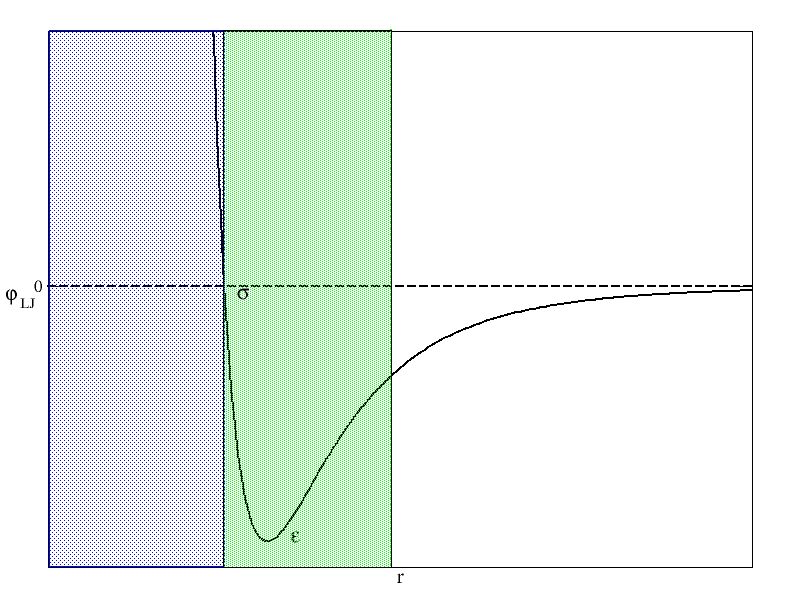
\includegraphics[width=.7\textwidth,keepaspectratio=true]{StatMech/LJfig.png}
    \caption{Potencial Lennard-Jones}
    \label{fig:LJ126}
\end{figure}

\newpage

Como se observa en la figura \ref{fig:LJ126}, el intervalo mostrado como el recuadro azul corresponde al potencial repulsivo, esta zona de la curva es donde se evita el traslape de las nubes electrónicas. El segundo intervalo mostrado como el recuadro verde es el pozo de potencial debido a la cohesión en la fase condensada de la materia.\\

\subsection{Interacción de Coulomb}

La interacción de Coulomb es la que existe entre cargas eléctricas y es la más fuerte de las interacciones y a veces tan fuerte como los enlaces químicos, el potencial depende inversamente de la distancia como se puede observar en la ecuación (\ref{coulombforce}) \cite{ISRAELACHVILI201153}.

\begin{equation} \label{coulombforce}
    \varphi(r_{ij}) = \left(\frac{q_i q_j}{4\pi \epsilon_{0} r_{ij}}\right)
\end{equation}

\noindent con $i\neq j$ donde $q_i$ y $q_j$ son las cargas de la i-ésima y j-ésima partícula respectivamente, $\epsilon_0$ es la permitividad eléctrica del vacío y $r_{ij}$ la distancia entre las partículas i, j. 


% \begin{enumerate}
%     \item El primer intervalo es el potencial repulsivo que está antes de la linea roja en la figura \ref{fig:LJ126}, este es para evitar el traslape de nubes electrónicas (Principio de exclusión de pauli).
%     \item El pozo del potencial es debido a la cohesión en la fase condensada de la materia.
%     \item La parte atractiva de este potencial es causada por la interacción de van der waals.
% \end{enumerate}

% \begingroup
% \let\clearpage\relax

\chapter{Dinámica molecular}
% \endgroup

La imposibilidad de hacer cálculos analíticos de las ecuaciones en la mecánica estadística como método para estudiar fluidos interactuantes, junto con la oportunidad de usar la aproximación Born-Oppenheimer(aproximación para escribir el hamiltoniano en términos de sus interacciones nucleares donde sus movimientos de electrones han sido promediados) abrió la posibilidad de simular computacionalmente sistemas interactuantes. El almacenamiento de datos y la alta capacidad de procesamiento de las computadoras actuales permiten resolver las ecuaciones de movimiento de Newton para sistemas atómicos.\\

\begin{figure}[!h]
    \centering
    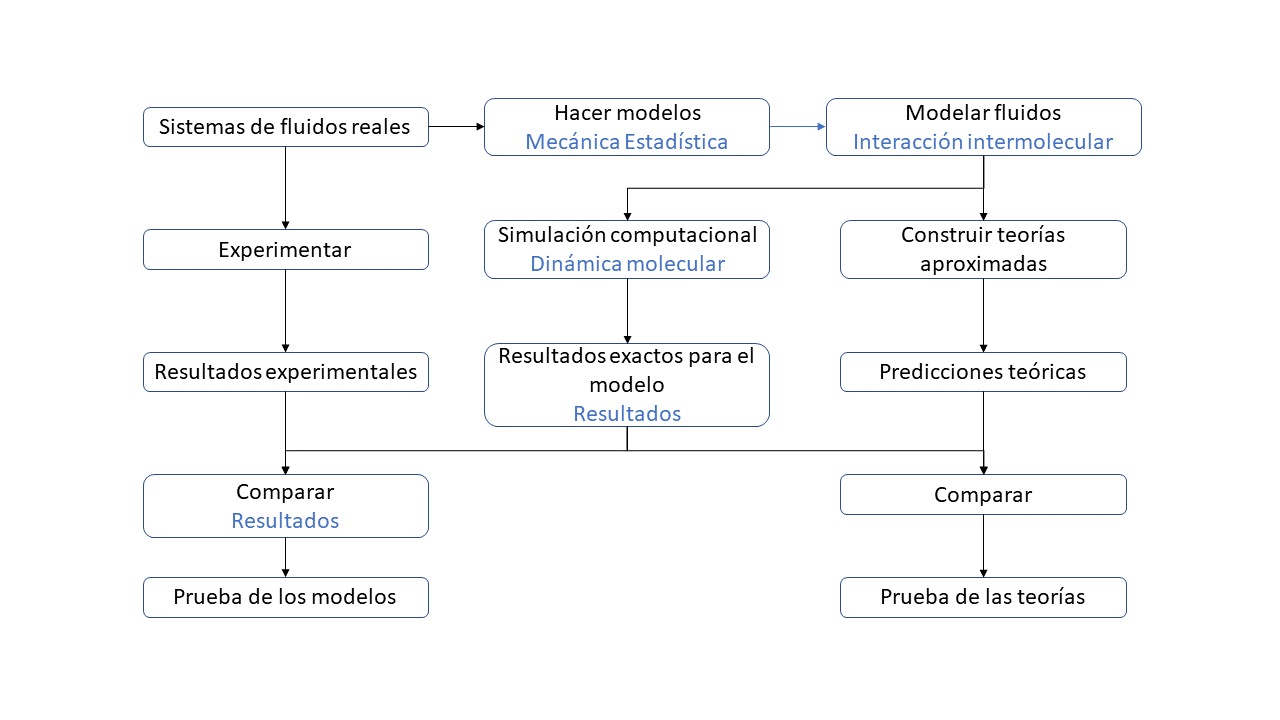
\includegraphics[width=.8\textwidth,keepaspectratio=true]{MD/experimentsimulationtheoryfig.png}
    \caption{Relación entre teoría, experimentación y simulación molecular. Figura adaptada de \cite{Allen2017}. Los capítulos de este trabajo están en color azul.}
    \label{fig:conteexpsim}
\end{figure}

La simulación vincula los resultados experimentales con los modelos de simulación y viceversa, mediante las propiedades termodinámicas del sistema como se muestra en la figura \ref{fig:conteexpsim}. La simulación molecular de un sistema nos permite introducir detalles microscópicos de los átomos y moléculas como geometrías, masas, interacciones, entre otros.\\

\section{Fundamentos de dinámica molecular}

La dinámica molecular resuelve las ecuaciones de movimiento descritas en la sección \ref{MecClasNpart} para un sistema atómico, molecular o centros de masa de configuraciones moleculares. Las ecuaciones de movimiento clásicas de Newton, están dadas por\\

\begin{equation}
    \mathbf{\dot p}_i = -\nabla_{\mathbf{r}_i} \varphi = \mathbf{F}_i
\end{equation}\\

\section{Métodos de diferencias finitas}

Las computadoras resuelven algoritmos, es decir, son operaciones de pasos que en este caso resuelven ecuaciones diferenciales. Es por esto que es necesario discretizar las ecuaciones de movimiento para tener una serie de pasos que la computadora resuelva por nosotros. La solución de las ecuaciones de movimiento se puede obtener numéricamente con métodos de diferencias finitas. Existen diferentes algoritmos que son computacionalmente eficientes.\cite{Allen2017}\\

Los algoritmos de integración usados en este trabajo son sencillos de derivar. Primero, se realiza una expansión de McLaurin de la posición, velocidad y aceleración alrededor del paso $\delta t$:

\begin{align} \label{taylorexpr}
\begin{split}
    \mathbf{r}(t + \delta t) &= \mathbf{r}(t)+\delta t\ \dot{\mathbf{r}}(t) + \frac{1}{2}\delta t^2\  \ddot{\mathbf{r}}(t)+...\\
                             &= \mathbf{r}(t)+\delta t\ \mathbf{v}(t) + \frac{1}{2}\delta t^2\ \mathbf{a}(t)+...
\end{split}
\end{align}
\begin{equation}\label{taylorexpv}
    \mathbf{v}(t + \delta t) = \mathbf{v}(t)+\delta t\ \mathbf{a}(t) + \frac{1}{2}\delta t^2\ \mathbf{j}(t)+...
\end{equation}
\begin{equation}\label{taylorexpa}
    \mathbf{a}(t + \delta t) = \mathbf{a}(t)+\delta t\ \mathbf{j}(t) + \frac{1}{2}\delta t^2\ \dot{\mathbf{j}}(t)+...
\end{equation}\\

\subsection{Algoritmo de Verlet}

El primer algoritmo para resolver ecuaciones de movimiento fue el de Verlet, este se hizo calculando series de McLaurin de $\mathbf{v}(t+\frac{1}{2}\delta t)$ y $\mathbf{r}(t-\delta t)$, y despues despreciamos términos $\delta^2$.\\

\begin{equation}\label{taylorexpr-}
    \mathbf{r}(t - \delta t) = \mathbf{a}(t)+\delta t\ \mathbf{j}(t) + \frac{1}{2}\delta t^2\ \mathbf{\dot{j}}(t)-...
\end{equation}

La ecuación (\ref{verletv1/2}) es la primera ecuación de Verlet:\\
\begin{equation}\label{verletv1/2}
    \mathbf{v}(t + \frac{1}{2}\delta t) = \mathbf{v}(t)+\frac{1}{2}\delta t\ \mathbf{a}(t)
\end{equation}\\

Sustituyendo la ecuación (\ref{verletv1/2}) en la ecuación (\ref{taylorexpr}) obtenemos la segunda ecuación de Verlet:

\begin{align} \label{verletr}
\begin{split}
    \mathbf{r}(t + \delta t) &= \mathbf{r}(t)+\delta t\ \dot{\mathbf{r}}(t) + \frac{1}{2}\delta t^2\ \ddot{\mathbf{r}}(t)+...\\
                             &= \mathbf{r}(t)+\delta t\ \left[\mathbf{v}(t) + \frac{1}{2}\delta t\ \mathbf{a}(t)\right]\\
                             &= \mathbf{r}(t)+\delta t\ \mathbf{v}(t+\frac{1}{2}\delta t)
\end{split}
\end{align}

Sustituyendo las ecuaciones (\ref{verletv1/2}) y (\ref{taylorexpa}) en la ecuación (\ref{taylorexpv}) obtenemos la tercera ecuación de Verlet:

\begin{align} \label{verletv}
\begin{split}
    \mathbf{v}(t + \delta t) &= \mathbf{v}(t)+\delta t\ \mathbf{a}(t) + \frac{1}{2}\delta t^2\ \mathbf{j}(t)+...\\
                             &= \mathbf{v}(t)+\frac{1}{2}\delta t\ \mathbf{a}(t) + \frac{1}{2}\delta t\ \mathbf{a}(t)+ \frac{1}{2}\delta t^2\ \mathbf{j}(t)+...\\
                             &= \mathbf{v}(t + \frac{1}{2}\delta t) + \frac{1}{2}\delta t\ \mathbf{a}(t + \delta t)
\end{split}
\end{align}

Pasos del algoritmo:

\begin{enumerate}
    \item Calcular la ecuación (\ref{verletv1/2}).
    \item Con el resultado del paso anterior, calcular la ecuación (\ref{verletr}).
    \item Calcular las fuerzas sobre la partícula para obtener la aceleración en $t + \delta t$.
    % \item $t = t + \delta t$
    % \item Regresamos al primer paso
\end{enumerate}

También si se quiere obtener la energía cinética se deriva la siguiente formula de la velocidad usando (\ref{taylorexpv}) y (\ref{taylorexpr-}):

\begin{equation}
    \mathbf{v}(t)=\frac{\mathbf{a}(t + \delta t)-\mathbf{r}(t - \delta t)}{2\delta t}
\end{equation}

\subsection{Algoritmo salto de rana}

El algoritmo de salto de rana es otra representación de las ecuaciones del algoritmo de Verlet, la ventaja de este algoritmo es que mejora la exactitud de la trayectoria calculada cuando se incorporan termostatos y barostatos a las ecuaciones de movimiento \cite{gromacsdoc}\cite{Allen2017}, es usado en este trabajo. Sus ecuaciones son\\

\begin{equation} \label{leapfrogv1/2}
    \mathbf{v}(t + \frac{1}{2}\delta t)=\mathbf{v}(t - \frac{1}{2}\delta t)+\delta t\mathbf{a}(t)
\end{equation}

\begin{equation} \label{leapfrogr}
    \mathbf{r}(t + \delta t)= \mathbf{r}(t)+\delta t \mathbf{v}(t+\frac{1}{2}\delta t)
\end{equation}

Pasos del algoritmo salto de rana:

\begin{enumerate}
    \item Calculamos la fuerza sobre la partícula al tiempo $t$.
    \item Calcular la ecuación (\ref{leapfrogv1/2}).
    \item Calcular la siguiente posición al tiempo $t+\delta t$ (\ref{leapfrogr}).
    % \item $t = t + \delta t$
    % \item Regresamos al primer paso
\end{enumerate}

\begin{figure}[!h]
    \centering
    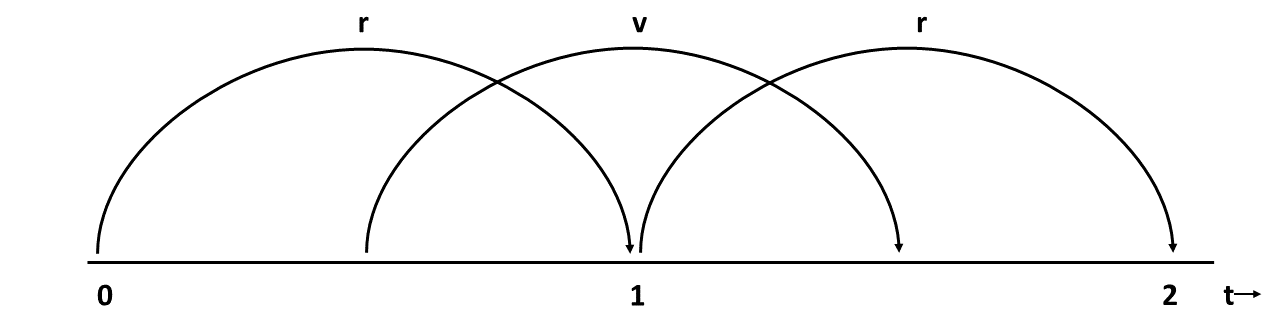
\includegraphics[width=.8\textwidth,keepaspectratio=true]{MD/leapfrogfig.png}
    \caption{Método de integración salto de rana, figura adaptada de \cite{gromacsdoc}.}
    \label{fig:leapfrog}
\end{figure}

\section{Condiciones de frontera periódicas y convención de mínima imagen}

Dentro del marco de simulación usado en esta tesis debemos considerar los elementos que se describen enseguida. Supongamos un cubo de simulación de longitud L, si se deseara realizar una simulación del sistema se necesitaría establecer la interacción molécula-pared. Para evitar estas interacciones empleamos condiciones de frontera periódicas: cuando una partícula deja el cubo, su imagen entra por la cara opuesta como en la figura \ref{fig:PBC}\\

\begin{figure}[!h]
    \centering
    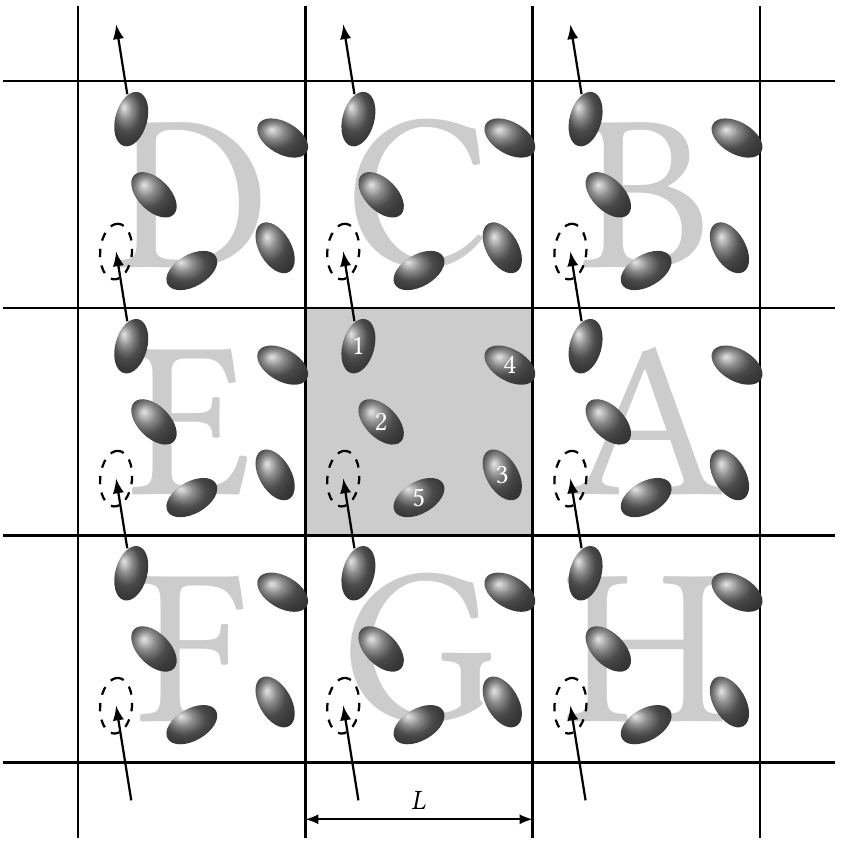
\includegraphics[width=.7\textwidth,keepaspectratio=true]{PBC.png}
    \caption{Un sistema periódico bidimensional, figura adaptada de \cite{Allen2017}.}
    \label{fig:PBC}
\end{figure}

\newpage

Las condiciones de frontera periódicas simulan la región de bulto, donde las paredes del contenedor no tienen influencia. El problema de usar estas condiciones es que al calcular el potencial o la fuerza entre pares se podría tomar en cuenta la fuerza de una partícula consigo misma, esto está prohibido por la ecuación (\ref{hamiltoniano}).

Para evitar este problema truncamos la distancia a la cual las partículas interaccionan e introducimos el llamado radio de corte, $r_c$, de tal manera que

\begin{equation}\label{MIC}
    \varphi(\mathbf{r}_{ij}) =
    \begin{cases} 
    \varphi(\mathbf{r}_{ij}),& \text{si } r_{ij}\leq r_c\\
    0,& \text{si } r_{ij}\geq r_c
    \end{cases}
\end{equation}\\

El valor máximo que $r_c$ puede tomar es $\frac{L}{2}$, de esta manera las partículas interaccionan con partículas en la celda original o con partículas imagen en celdas replicadas con la condición de que estén a la mínima distancia.\\

Con estas dos consideraciones podemos evitar hacer simulaciones con un número de moléculas del orden de $10^{23}$, además de que no es factible con la capacidad de cómputo actual. La condición de frontera periódica simula un bulto de moléculas y la convención de mínima imagen elimina la influencia de una molécula consigo misma y con otras a distancias en la que el potencial es despreciable, esto hace innecesario agregar tantas moléculas.\\

\section{Termostato de Nosé-Hoover}

Para incorporar en el sistema propiedades termodinámicas fijas, es necesario el uso de ``dispositivos'' que afecten la dinámica del sistema de tal manera que cuando midamos estas propiedades, veamos que se encuentran fijos. Para mantener fija la temperatura se usa un termostato, en este caso derivamos el termostato de Nosé y Hoover. Este termostato extiende el hamiltoniano del sistema introduciendo un baño térmico y un término de fricción a las ecuaciones de movimiento. La fricción es proporcional al producto de la velocidad de cada partícula y una coordenada de fricción $\xi$(esta es una cantidad dinámica con su propio momento $p_\xi$)\cite{evans1985} \cite{gromacsdoc}. Las ecuaciones de movimiento para una partícula en un sistema con este termostato son reemplazadas por:\\

\begin{equation} \label{NHmotion}
    \frac{d^2\mathbf{r}_i}{dt^2} = \frac{\mathbf{F}_i}{m_i}-\frac{p_\xi}{Q}\frac{d\mathbf{r}_i}{dt},
\end{equation}\\

\noindent donde $Q=\frac{\tau_T^2 T_0}{4\pi^2}$.\\

La energía cinética está relacionada a la temperatura del sistema, en otros termostatos se reescala la velocidad considerando un término multiplicado por la velocidad o tomando velocidades de una distribución de probabilidades de Maxwell. Esos termostatos no representan estrictamente un ensamble isotérmico, pero son útiles para muchos propósitos ya que producen prácticamente las mismas propiedades que el termostato de Nosé-Hoover. El termostato de Nosé-Hoover si representa a un ensamble isotérmico y la cantidad dinámica que se mete en las ecuaciones de movimiento de las partículas, representa la influencia del baño térmico.\\

La ecuación de movimiento para la coordenada $\xi$ del baño térmico es:\\

\begin{equation}
    \frac{dp_\xi}{dt}=(T-T_0),\quad T_0\ es\ la\ temperatura\ de\ referencia.
\end{equation}\\

La cantidad conservada para las ecuaciones de Nosé-Hoover es:\\

\begin{equation} \label{conservedNoseHoover}
    \mathcal{H} = \sum_{i=1}^{N}\frac{\mathbf{p}_i^2}{2m_i} + U(\mathbf{r}_1,...,\mathbf{r}_N)+\frac{p_\xi^2}{2Q} + N_fKT\xi
\end{equation}\\

\noindent donde $\tau_T$ es un parámetro dentro de la simulación y $N_f$ es el número de grados de libertad del sistema.\\

El termostato de Nosé-Hoover permite una relajación oscilatoria a la temperatura de referencia por lo que tarda mas tiempo que otros termostatos en llegar a la temperatura impuesta.\\

\section{Barostato de Parrinello-Rahman}

Al igual que con el termostato, si queremos incorporar una presión fija al sistema, es necesario incorporar un barostato a las ecuaciones. En esta sección derivamos el barostato de Parrinello-Rahman usado en la simulación, en este barostato los vectores de la caja están representados por $\mathbf{b}$ y obedecen la ecuación de movimiento matricial\cite{gromacsdoc} \cite{simone1993}:\\

\begin{equation} \label{parrrahman}
    \frac{d\mathbf{b}^2}{dt^2}=V\mathbf{W}^{-1}\mathbf{b'}^{-1}(\mathbf{P}-\mathbf{P}_{ref})
\end{equation}\\

\noindent donde V es el volumen de la caja, $\mathbf{W}$ es la matriz de parámetros que determina la fuerza de acoplamiento y las matrices $\mathbf{P},\mathbf{P}_{ref}$ son la presión instantánea y la presión de referencia respectivamente. Este barostato se usa comúnmente en combinación con el termostato Nosé-Hoover. Así las ecuaciones de movimiento y la cantidad conservada $\mathcal{H}$ son \cite{gromacsdoc}:

\begin{equation} \label{NHPRmotionr}
    \frac{d^2\mathbf{r}_i}{dt^2} = \frac{\mathbf{F}_i}{m_i}-\mathbf{M}\frac{d\mathbf{r}_i}{dt}
\end{equation}
con $\mathbf{M}=\mathbf{b}^{-1}\left[\mathbf{b}\frac{d\mathbf{b'}}{t}+\frac{d\mathbf{b}}{dt}\mathbf{b'}^{-1} \right]$
% \begin{equation} \label{NHPRmotionV}
%     \frac{d^2 b}{dt^2} = \frac{\dot{\xi}\dot{V}}{\xi} + \xi^2\mathbf{W}^{-1}(\mathbf{P}-\mathbf{P}_{ref})
% \end{equation}
\begin{equation} \label{conservedNoseHooverParrRahm}
    \mathcal{H} = \sum_{i=1}^{N}\frac{\mathbf{p}_i^2}{2m_i} + U(\mathbf{r}_1,...,\mathbf{r}_N) + \sum_i P_{ii}V + \sum_{i,j}\frac{1}{2}W_{ij}\left(\frac{db_{ij}}{dt}\right)^2
\end{equation}\\

\noindent con $\mathbf{W}^{-1}_{ij}=\frac{4\pi^2 \beta_{ij}}{3\tau_{p}^2 L}$, $\tau_p$ el parámetro de acoplamiento del barostato en la simulación y L la longitud de la celda de simulación que en este caso es un cubo.

\section{Campos de fuerzas}

El campo de fuerzas en una simulación es la energía potencial total del sistema alimentada por un conjunto de parámetros. Su forma funcional es fundamental ya que de ella se derivan las fuerzas que experimentan las partículas en el fluido. La forma funcional del campo de fuerzas contiene los términos de interacción que se describen enseguida.\\

\subsection{Potencial de enlace}

Modela la distancia de enlace entre átomos de una molécula. Hay dos importantes que usan en la simulación del sistema de esta tesis. El potencial de enlace usado en el modelo del agua SPCE es el armónico \cite{gromacsdoc}:

\begin{equation}
    \varphi_{enlaces}(r_{ij}) = \frac{1}{2}k_{ij}^{b}(r_{ij} - b_{ij})^2
\end{equation}

\noindent con $k_{ij}$ es la constante del enlace con unidades $\frac{kJ}{mol\ nm^2}$ y $b_{ij}$ la distancia entre el par en nm.\\

Para los demás moléculas, el potencial es la de cuarta potencia \cite{gromacsdoc}:

\begin{equation}
    \varphi_{enlaces}(r_{ij}) = \frac{1}{4}k_{ij}^{b}(r_{ij}^2 - b^{2}_{ij})^2
\end{equation}

\noindent donde $k_{ij}$ es la constante del enlace con unidades $\frac{kJ}{mol\ nm^4}$ y $b_{ij}$ la distancia entre ellos en nm.\\

\begin{figure}[!h]
    \centering
    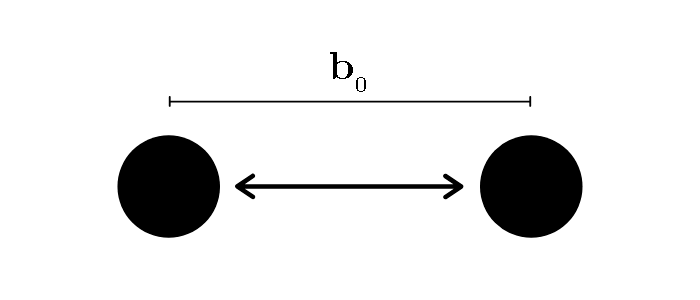
\includegraphics[width=.4\linewidth]{MD/bondpotential.png}  
    \caption{Figura representativa del potencial de enlace entre dos átomos a una distancia $b_0$.}
    \label{fig:bondpotential}
\end{figure}

Como ejemplo, la distancia de enlace entre el par O-H en agua es de $b=1$\AA\ y con constante de enlace de $k=345000\ \frac{kJ}{mol\ nm^2}$.

\subsection{Potencial del ángulo de enlace}

El potencial de ángulo modela el ángulo de enlace entre átomos de una molécula, el usado en este trabajo fue el potencial de ángulo basado en coseno \cite{gromacsdoc}.

\begin{equation}
    \varphi_{ángulo}(\theta_{ijk}) = \frac{1}{2}k^{\theta}_{ijk}\left(cos(\theta_{ijk}) - cos(\theta^{0}_{ijk})\right)^2,
\end{equation}

\noindent donde $k^{\theta}_{ijk}$ es la constante de fuerza con unidades $\frac{kJ}{mol}$ y $\theta_{ijk}$ es el ángulo de enlace.\\

\begin{figure}[!h]
    \centering
    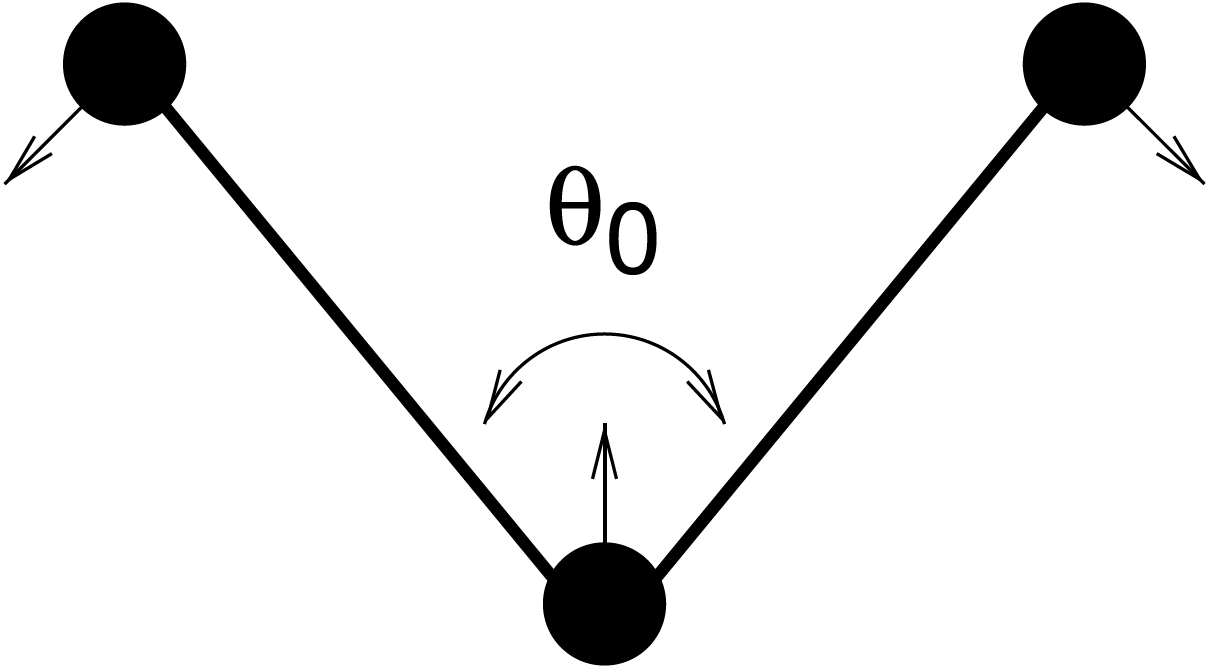
\includegraphics[width=.4\linewidth]{MD/anglepotential.png}  
    \caption{Figura representativa del potencial del ángulo de enlace entre tres átomos con un ángulo $\theta_0$. Figura tomada de \cite{gromacsdoc}.}
    \label{fig:anglepotential}
\end{figure}

\subsection{Potencial de ángulos diedros impropio y propio}

Los potenciales de ángulos diedros modelan el angulo entre dos planos. Los diedros impropios es cuando 3 átomos pertenecen al mismo plano y el cuarto rota de manera solitaria en otro plano con respecto a dos de los átomos del otro plano como se muestra en la figura \ref{fig:improperdihedralanglepotential}. Los ángulos diedros propios son como se muestra en la figura \ref{fig:properdihedral}.

\begin{figure}[!h]
\imagewidth=0.6\textwidth
\captionsetup[subfigure]{width=0.7\imagewidth,justification=raggedright}
\begin{subfigure}{.5\textwidth}
  \centering
  % include first image
  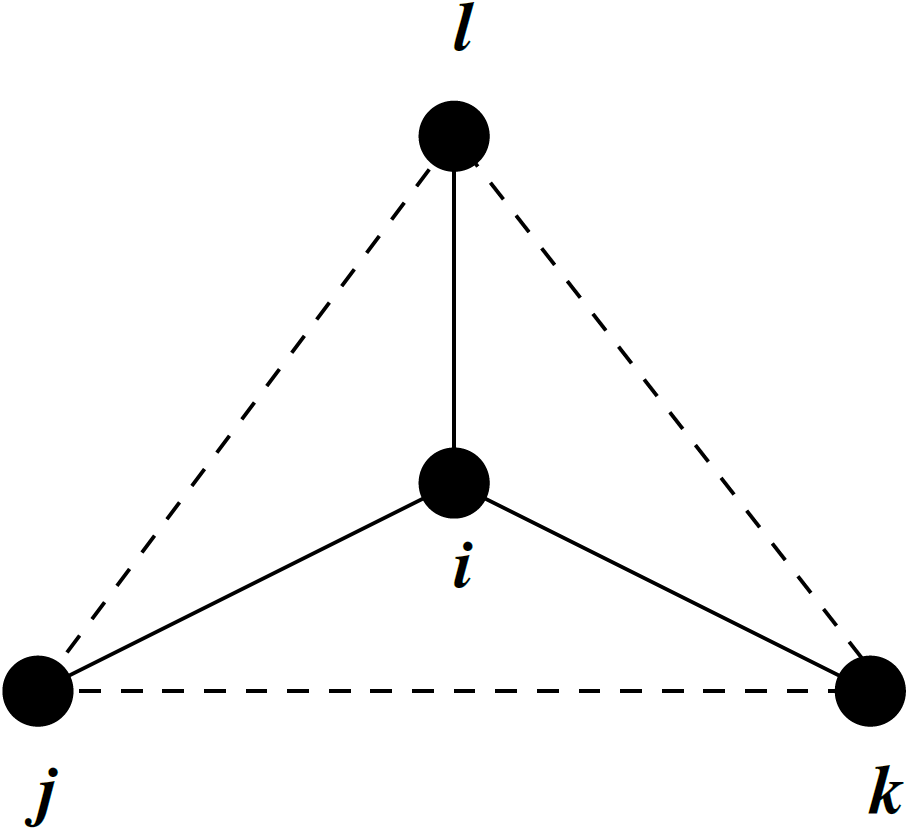
\includegraphics[width=.7\linewidth]{MD/improperdihedralanglepotential2.png}  
  \caption{Figura representativa del uso del potencial de diedros impropios. Figura tomada de \cite{gromacsdoc}.}
  \label{fig:improperdihedralanglepotential}
\end{subfigure}
\begin{subfigure}{.5\textwidth}
  \centering
  % include second image
  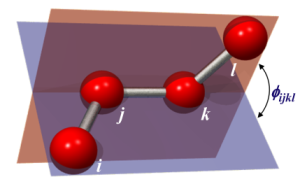
\includegraphics[width=.8\linewidth]{MD/properdihedral.png}  
  \caption{Ángulo formado en un diedro propio. Figura tomada de \cite{charmmgui}}
  \label{fig:properdihedral}
\end{subfigure}
% \caption{Los potenciales de las fuerzas intermoleculares.}
% \label{fig:intermolecularpotential}
\end{figure}

\subsection{Campo de fuerzas GROMOS54A7}

Para este trabajo se usó el campo de fuerzas GROMOS54A7 que se muestra a continuación:

\begin{equation}
\begin{split}
    &\varphi_{GROMOS}\\ & = \sum_{enlaces}\frac{1}{4}k_{ij}^{b}(r_{ij}^2 - b^{2}_{ij})^2 + \sum_{angulos} \frac{1}{2}k^{\theta}_{ijk}\Big(cos(\theta_{ijk}) - cos(\theta^{0}_{ijk})\Big)^2\\ 
    &+ \sum_{diedros\ impropios}\frac{1}{2}k^{\xi}_{ijkl}(\xi_{ijkl} - \xi_{0})^2 + \sum_{diedros}k^{\phi}_{ijkl}\Big(1 + cos(n\phi_{ijkl} - \phi^{s}_{ijkl}) \Big)\\ 
    &+ \sum_{pares\ átomos}\left[4\epsilon_{ij} \left[\left(\frac{\sigma_{ij}}{r_{ij}} \right)^{12} - \left(\frac{\sigma_{ij}}{r_{ij}}\right)^6 \right] + \left(\frac{q_i q_j}{4\pi \epsilon_{0} r_{ij}}\right)\right]
    \end{split}
\end{equation}

Con $n=2$ en los ángulos diedros propios, al menos que se especifique lo contrario en el apéndice \ref{chapter:apendicea}.\\

% \begin{align*}\label{FF}
%     U_{conf} &= \sum_{enlaces}K_r\left(r-r_0\right)^2 + \sum_{angulos}K_{\theta}\left(\theta-\theta_0\right)^2 \\
%              &+ \sum_{diedros}K_{\phi}\left[1-cos(n\phi-\delta)\right] \\
%              &+ \sum_{diedros\ impropios}K_{\omega}\left(\omega-\omega_0\right)^2 + \sum_{cargas}\left(\frac{q_i q_j}{4\pi \epsilon r^2_{ij}}\right) \\
%              &+ \sum_{VdW} 4 \epsilon_{ij}\left[\left(\frac{\sigma_{ij}}{r_{ij}}\right)^{12}-\left(\frac{\sigma_{ij}}{r_{ij}}\right)^{6}\right]    
% \end{align*}

% La siguiente tabla \ref{FFallen} muestra otros campos de fuerzas:

% \begin{table}[h!]
%     \centering
%     \begin{tabular}{l c l}
%     \hline
%     Campo de Fuerza & Clase & Dominio \\
%     \hline
%     OOPLS & I & péptidos y pequeños orgánicos \\
%     CHARM27 & I & ADN, ARN y lípidos \\
%     GAFF & I & pequeños orgánicos y diseño de drogas \\
%     GROMOS ffG45a3 & I & lípidos y micelas\\
%     clayFF & II & minerales hidratados \\
%     AMBER ff02 & III & átomos polarizables \\
%     AMOEBA & III & multipolos polarizables y multipolos distribuidos \\
%     MARTINI & III & modelos de grano grueso, proteinas, lípidos y polímeros \\
%     \hline
%     \end{tabular}
%     \caption{Ejemplo de campo de fuerzas, dominios de aplicación y clases\cite{Allen2017}}
%     \label{FFallen}
% \end{table}

% \begin{itemize}
%     \item Tipo I: son potenciales parametrizados para cada tipo de átomo en el sistema.
%     \item Tipo II: potenciales parametrizados para todos los átomos incluyendo términos cúbicos en enlaces y otros.
%     \item Tipo III: potenciales parametrizados para todos los átomos extendiendo los cálculos electrostáticos para incluir polarización. Estos también incluyen a los campos de grano grueso.
% \end{itemize}



\chapter{Propiedades calculadas}

En este capítulo se describen las ecuaciones y los métodos usados para extraer resultados del sistema estudiado. En particular describimos la función de distribución radial, el número de coordinación, coeficiente de difusión,  la temperatura, energía y presión. Al final de este capítulo se detalla el sistema simulado.

\section{Función de distribución radial y número de coordinación}
% \textcolor{red}{usar mejor la definición de VMD para enlazar bien el marco teórico con la metodología}

Esta función es importante ya que proporciona información estructural promedio del sistema.\\

Esta función da la probabilidad de encontrar un par de átomos a distancia r, relativa a la probabilidad de una distribución completamente aleatoria a la misma densidad. En la dinámica molecular, la función de distribución radial se calcula usando la relación (\ref{gr})\\

\begin{equation} \label{gr}
    g(r)=\lim_{dr\to 0} \frac{\left<N(r, r+dr)\right>}{\frac{4 \pi}{3} \rho \left[(r+dr)^3 - r^3\right]}
\end{equation}\\

\noindent donde $r$ es la distancia entre átomos, $\left<N(r, r+dr)\right>$ es el número promedio de átomos encontrados a una distancia entre $r$ y $r + dr$, $\rho$ es la densidad total del sistema.

El promedio $\left<N(r, r+dr)\right>$ es calculado sobre toda la trayectoria de una simulación.

\begin{figure}[!h]
    \centering
    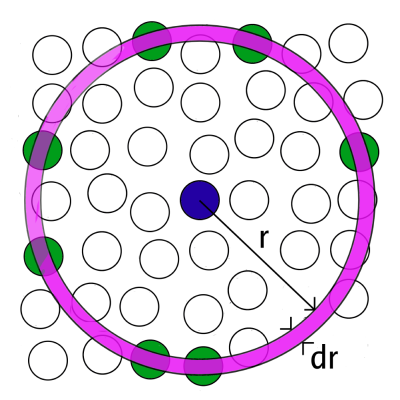
\includegraphics[width=.2\textwidth,keepaspectratio=true]{gr.png}
    \caption{Evaluación de la función de distribución radial}
    \label{fig:gr}
\end{figure}

% \begin{equation} \label{gr}
%     g(r)=\lim_{dr\to 0} \frac{p(r)}{4\pi \left(N_{pares}/V\right)r^{2}dr}
% \end{equation}\\

% donde $r$ es la distancia entre átomos, $p(r)$ es el promedio del número de pares de átomos encontrados a una distancia entre $r$ y $r+dr$, V el volumen total del sistema y $N_{pares}$ es el número de pares únicos de átomos donde un átomo es de cada uno de dos conjuntos, $sel_1$ y $sel_2$.\\

% \begin{figure}[!h]
%     \centering
%     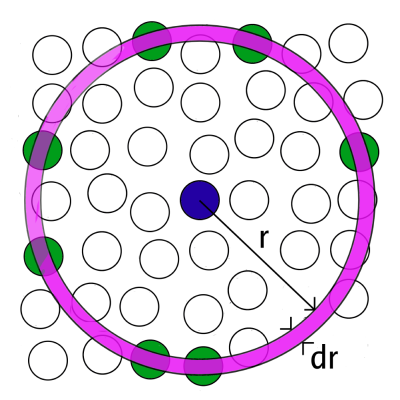
\includegraphics[width=.2\textwidth,keepaspectratio=true]{gr.png}
%     \caption{Evaluación de la función de distribución radial}
%     \label{fig:gr}
% \end{figure}

% El promedio $p(r)$ es calculado sobre toda la trayectoria de una simulación con $N_{cuadros}$ el número total de cuadros en la simulación. Este promedio toma la forma de:\\

% \begin{equation}\label{p}
%     p(r)=\frac{1}{N_{cuadros}}\sum^{N_{cuadros}}_i \sum_{j\in sel1} \sum_{k\in sel2} \sum_{\kappa} d_{\kappa}(r_{ijk})
% \end{equation}\\

% donde $\kappa$ son los índices de los contenedores del histograma y

% \begin{equation}
%     d_{\kappa}(r_{ijk}) = 
%     \begin{cases}
%         1 / \Delta r &\text{si $r_\kappa \leqq r<r_\kappa + \Delta r$ y $r_\kappa \leqq r_{ijk}<r_\kappa + \Delta r$}\\
%         0 & \text{de otra manera}\\
%     \end{cases}
% \end{equation}

% donde $\Delta r$ es el ancho de los contenedores del histograma y $r_\kappa$ es la distancia mínima asociada con cada contenedor, dado por:

% \begin{equation}
%     r_\kappa = r_0 + \kappa \Delta r
% \end{equation}

% con $r_0$ el límite inferior del histograma.\\

% El cálculo de la función de distribución radial también cumple con la convención de mínima imagen. El límite superior del histograma debería no ser mayor a $L/2$.\\

El número de coordinación se calcula como

\begin{equation}
    N(r) =  \int_0^{r_m} \rho g(r)4\pir^{2}dr
\end{equation}

\noindent donde $r_m$ es la distancia en que se encuentra el primer mínimo de $g(r)$ y $\rho$ es la densidad de bulto del sistema. Este es un promedio del número de vecinos hasta $r_m$ \cite{GOCHENOUR201841}. Para el caso de la simulación, es el promedio en todos los cuadros.\\

\section{Propiedades macroscópicas del sistema}

\subsection{Energía}

El promedio de la energía se calcula como el promedio de la ecuación (\ref{hamiltoniano}) \cite{Allen2017}:

\begin{equation} \label{promenergia}
    \langle E \rangle = \left \langle\sum_{i=1}^{N} \frac{1}{2 m_i}\dot{\mathbf{p}}_i^2 \right \rangle+ \left \langle\sum_{i=1}^{N-1}\sum_{j=i+1}^{N} u(r_{ij})\right \rangle
\end{equation}

\subsection{Temperatura}

Aunque la temperatura se mantiene fija en la simulación proporcionamos su descripción \cite{Allen2017}.

\begin{equation} \label{virialtheorem}
    \left \langle p_k \frac{\partial H}{\partial p_k} \right \rangle = k_B T.
\end{equation}

Para el hamiltoniano en la ecuación (\ref{hamiltoniano}) encontramos:

\begin{equation} \label{virialtemp}
    k_B T = \left \langle p_k \frac{p_k}{m_k} \right \rangle
\end{equation}

\noindent entonces derivamos la siguiente ecuación al incorporar la suma para los 3N términos de N partículas:

\begin{equation} \label{virialsumtemp}
    3Nk_B T = \left \langle \sum_{k=1}^{N}\frac{|p_k|^2}{m_k} \right \rangle.
\end{equation}

Para un sistema donde hay $N_C$ restricciones de algún tipo (e.g. descripciones de centro de masa, ángulos rígidos, enlaces rígidos entre otros), la ecuación anterior se convierte en:

\begin{equation} \label{virialsumconsttemp}
    T= \frac{1}{3(N - N_C)k_B}\left \langle \sum_{k=1}^{N}\frac{|p_k|^2}{m_k} \right \rangle
\end{equation}

\subsection{Presión}

% La otra ecuación del teorema del virial nos da la siguiente ecuación:

% \begin{equation} \label{virialtheoremq}
%     \left \langle q_k \frac{\partial H}{\partial q_k} \right \rangle = k_B T
% \end{equation}

% lo cual nos lleva a:

% \begin{equation} \label{virialtheorempress}
%     \frac{1}{3}\left \langle \sum_{i=1}^N \mathbf{r_i} \cdot \mathbf{f}^{tot}_i \right \rangle = -N k_B T
% \end{equation}

% si dividimos la fuerza total entre externa e intermolecular llegamos a otra ecuación \cite{Allen2017}:

La presión promedio se determina considerando su contribución cinética y la parte debida a interacciones, a través de

\begin{equation} \label{virialsumconstpress}
    P = \frac{N}{\left \langle V \right \rangle} k_B T + \frac{\left \langle \mathcal{W} \right \rangle}{\left \langle V \right \rangle}
\end{equation}

\noindent donde $\mathcal{W} = \frac{1}{3} \sum_{i=1}^N \mathbf{r_i} \cdot \mathbf{f}_i$ con $\mathbf{f}_i$ fuerzas intermoleculares las cuales se obtienen a través del campo de fuerzas.

\section{Coeficiente de difusión}

% La ecuación de difusión describe como alguna variable se propaga en un sistema, por ejemplo, unir una barra metálica caliente con otra fría (conocida como la ecuación de difusión de calor).

% La difusión molecular puede interpretar como dos sistemas con diferentes temperaturas o variable termodinámica fluye hacia el equilibrio.

% Por la naturaleza molecular de un sistema, se puede modelar las interacciones de las moléculas como una caminata aleatoria(así ignoramos la interacción o la implicación de momentos, fuerzas, entre otros).

% Podemos hacer primero un modelo de esta caminata aleatoria de manera discreta en el espacio y tiempo hasta llevarlo de manera continua en espacio y tiempo tomando en cuenta el promedio del movimiento de partículas

% Primero describimos el modelo aleatorio en una dimensión. En una sección de recta numérica dejamos como ejemplo mil partículas (con distribución de 50-50 de moverse a ambos lados) distribuidas de igual manera a la mitad del lado izquierdo con una condición de frontera que si una partícula se encuentra en alguna de las frontera, su probabilidad es 50% y 50% en quedarse en el mismo lugar o moverse contrario a la frontera.

%En promedio mitad de la densidad lineal de partículas en un i-esimo delta x se movera hacia la izquierda y la otra mitad a la derecha y la mitad de la densidad lineal de los vecinos entrará

% En ecuación esto es, delta rho_i = 1/2[(rho_{i+1}-rho_{i})-(rho_{i}-rho_{i-1})]

% La constante de difusión da la idea de que tan rápido se mueven las partículas

Los coeficientes de transporte como el coeficiente de difusión describen la relajación de variables dinámicas en la escala macroscópica. Siempre considerando que el tiempo y los límites a gran escala son los adecuados, pueden ser descritos en términos de funciones de correlación de tiempo en equilibrio microscópicos \cite{Allen2017}. Para un sistema en equilibrio, el coeficiente de difusión de las partículas de tipo A, $D_A$, se obtiene a través de \cite{gromacsdoc}

\begin{equation} \label{diffusioncoeff}
    D_A = \frac{1}{6} \lim_{t \to \infty} \left\langle\left\| \mathbf{r}_{i}(t) - \mathbf{r}_{i}(0) \right\|^2 \right\rangle_{i \in A},
\end{equation}

\noindent es decir, el coeficiente de difusión está dado por el desplazamiento cuadrático medio del centro de masa de las posiciones de las moléculas. Este representa la movilidad de las moléculas en la solución, de igual manera que la conductividad eléctrica representa la de los electrones a través del material.\\

En el programa de simulación usado, se puede calcular el coeficiente de difusión de un grupo de moléculas o átomos \cite{gromacsdoc}.

\section{Sistema simulado}

El sistema se simuló en un rango de temperaturas de 280 a 370 K, que consta de 16807 moléculas de agua, 10 moléculas de ácido 2,4-diclorofenoxiacético (2,4-D) y un nanotubo de carbono (6, 5) con una longitud alrededor de 38nm. En todas las simulaciones se usó el termostato de Nosé-Hoover acoplado con un barostato Parrinello-Rahman con $\tau_t$ de 0.4 ps y $\tau_p$ de 1.6 ps, respectivamente.\\

Todas las simulaciones constaron de 20 ns de tiempo de simulación, se usó el algoritmo de salto de rana y radio de corte de 1.2 nm. La validez de los parámetros del termostato y barostato fue verificada revisando que las condiciones de simulación fueron mantenidas de manera adecuada conforme los valores impuestos en la simulación NPT, como se muestra en la tabla \ref{tab:promediostemppres}.

\begin{table}[h!]
    \centering
    \begin{tabular}{ |m{6em}|m{5em}||m{5em}|m{5em}|  }
    \hline
    Temperatura (K) & Error & Presión (bar) & Error \\
    \hline
    \hline
    280.003 & 0.0018 & 0.840079 & 0.12 \\
    298.149 & 0.0014 & 1.11589 & 0.099 \\
    309.998 & 0.0013 & 1.28056 & 0.2 \\
    319.996 & 0.0012 & 1.01285 & 0.12 \\
    329.998 & 0.0016 & 1.12986 & 0.079 \\
    340 & 0.0019 & 1.11812 & 0.13 \\
    349.998 & 0.0028 & 1.30148 & 0.13 \\
    360.003 & 0.0022 & 1.02411 & 0.13 \\
    370.002 & 0.002 & 1.1182 & 0.13 \\
    \hline
    \end{tabular}
    \caption{Promedio de temperatura y presión de los sistemas simulados. El error es calculado por el metodo de promedio de bloques \cite{gromacsdoc}.}
    \label{tab:promediostemppres}
\end{table}


% y el campo de fuerzas usado en el sistema es GROMOS 54A7, que tiene la siguiente forma en nuestras simulaciones:
% \begin{itemize}
%     \item Número de moléculas: 16807 moléculas de agua, 10 moléculas de ácido 2,4-diclorofenoxiacético (2,4-D) y un nanotubo de carbono (6, 5) con 364 átomos.
%     \item Integrador de todos los sistemas: salto de rana para las ecuaciones de movimiento de Newton.
%     \item Paso de tiempo: 0.002 ps, número de pasos: 10000000, Intervalo de tiempo: 20 ns.
%     \item radio de corte para la lista de vecinos de corto alcance: 1.2 nm, radio de corte para interacción de coulomb: 1.2 nm, radio de corte para interacción LJ 12-6: 1.2 nm.
%     \item Corrección de dispersión de largo alcance para energía y presión.
%     \item Acoplamiento de temperatura: ensamble extendido de nose-hoover con $\tau_t$: 0.4 ps y con las temperaturas antes mencionadas.
%     \item Acoplamiento de presión: ensamble extendido de parrinello-rahman con $\tau_p$: 1.6 ps a presión: 1 bar.
%     \item Algoritmo de constricción: LINCS(LINear Constraint Solver).
% \end{itemize}





\chapter{Resultados}

A continuación se presentan gráficas de propiedades estructurales y termodinámicas para analizar el sistema estudiado.

% \subsubsection{Propiedades termodinámicas}

% Se muestran algunas figuras que son cálculos instantáneos de la presión y temperatura:

% \begin{figure}[!h]
%     \centering
%     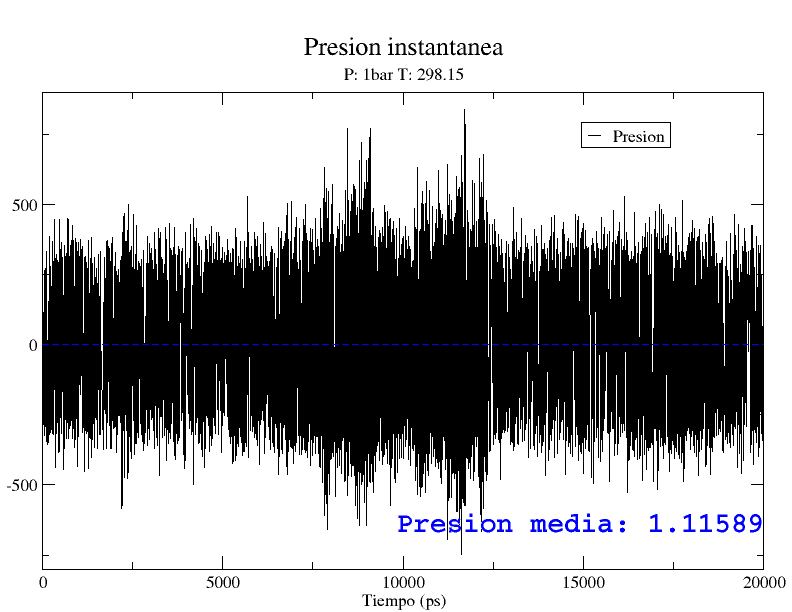
\includegraphics[width=.9\textwidth,keepaspectratio=true]{Pres298.png}
%     \caption{Gráfica de la presión instantánea del sistema a condición estandar IUPAC, la media de la presión fue 1.11589 bar}
%     \label{fig:Enertot298.15}
% \end{figure}
\section{Representación visual de la adsorción de las moléculas 2,4-D}

La figura \ref{fig:Conffinal370} es una representación visual de la adsorción de las moléculas 2,4-D en el nanotubo. Esta adsorción que se observa en la representación visual, se replica en todas las configuraciones finales del sistema en todas las temperaturas simuladas.

\begin{figure}[!h]
    \centering
    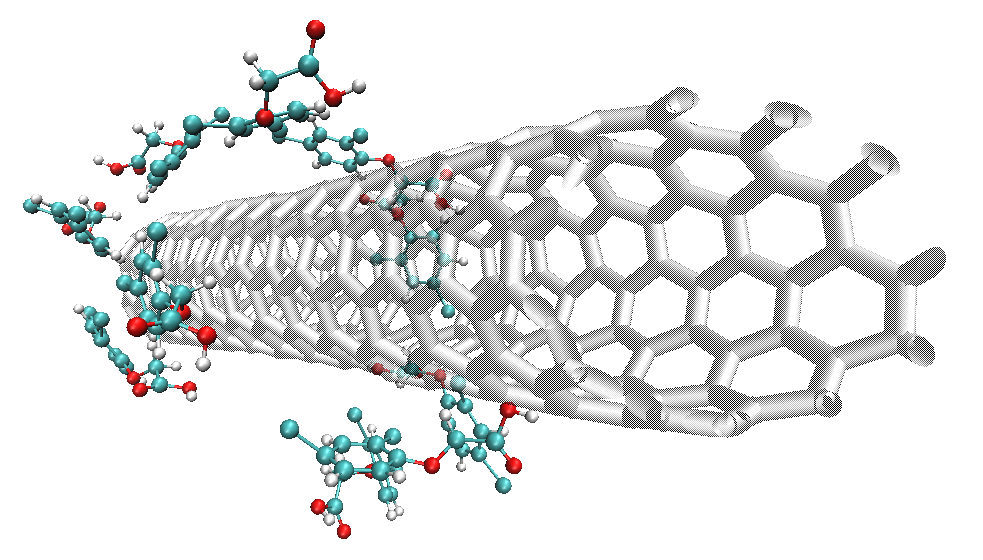
\includegraphics[width=0.6\textwidth,keepaspectratio=true]{resultados/all-new-370K.png}
    \caption{Nanotubo y moléculas de 2,4-D en la configuración final a 370 K.}
    \label{fig:Conffinal370}
\end{figure}

\section{Función de distribución radial}

Las funciones de distribución radial fueron calculado en un rango de 280 a 370. En el caso de pares átomo-átomo se calcularon los pares entre átomos de oxígeno-oxígeno, oxígeno-hidrógeno y hidrógeno-hidrógeno del agua, también los pares entre carbono del nanotubo de carbono y ácido 2,4-diclorofenoxiacético que son carbono-oxígeno de 2,4-D, carbono-hidrógeno de 2,4-D, carbono-cloro de 2,4-D y carbono-carbono de 2,4-D. Igualmente se calcularon los pares entre centro de masa del nanotubo y átomo de 2,4-D los cuales son centro de masa del nanotubo-oxígeno, centro de masa del nanotubo-hidrógeno, centro de masa del nanotubo-cloro y centro de masa del nanotubo-carbono. Además se calcularon la funciones para los pares centro de masa del nanotubo de carbono-centro de masa de la molécula 2,4-D y carbono del nanotubo-centro de masa de 2,4-D.\\

% \begin{itemize}
%     \item átomo A - átomo B:
%         \begin{itemize}
%             \item agua-agua: OW-OW, OW-HW, HW-HW
%         \end{itemize}
%         % \begin{itemize}
%         %     \item agua-2,4-D: OW-OD, OW-ClD, OW-HD, HW-HD, HW-ClD
%         % \end{itemize}
%         % \begin{itemize}
%         %     \item agua-CNT(6,5): OW-C,  HW-C
%         % \end{itemize}
%         \begin{itemize}
%             \item 2,4-D-CNT(6,5): OD-C, HD-C, ClD-C, CD-C
%         \end{itemize}
%         % \begin{itemize}
%         %     \item 2,4-D-2,4-D: OD-OD, HD-HD, ClD-ClD, CD-CD, ClD-HD, OD-HD
%         % \end{itemize}
%         % \begin{itemize}
%         %     \item CNT(6,5)-CNT(6,5): C-C
%         % \end{itemize}
%     \item centro de masa A - centro de masa B:
%         \begin{itemize}
%             \item 2,4-D-CNT(6,5): centro de masa CNT - centro de masa 2,4-D, centro de masa de ambas tapas CNT - centro de masa 2,4-D
%         \end{itemize}
%     \item centro de masa A - átomo B:
%         \begin{itemize}
%             \item CNT(6,5)-2,4-D: centro de masa CNT - ClD, centro de masa CNT - HD, centro de masa CNT - OD, centro de masa CNT - Cl1D
%         \end{itemize}
%         % \begin{itemize}
%         %     \item agua-2,4-D: OW-OD, OW-ClD, OW-HD, HW-HD, HW-ClD
%         % \end{itemize}
% \end{itemize}

% A continuación se presentan algunas gráficas y figuras significativas para posteriormente para analizar.\\

% \newpage

\begin{figure}[!hbt]
    \centering
    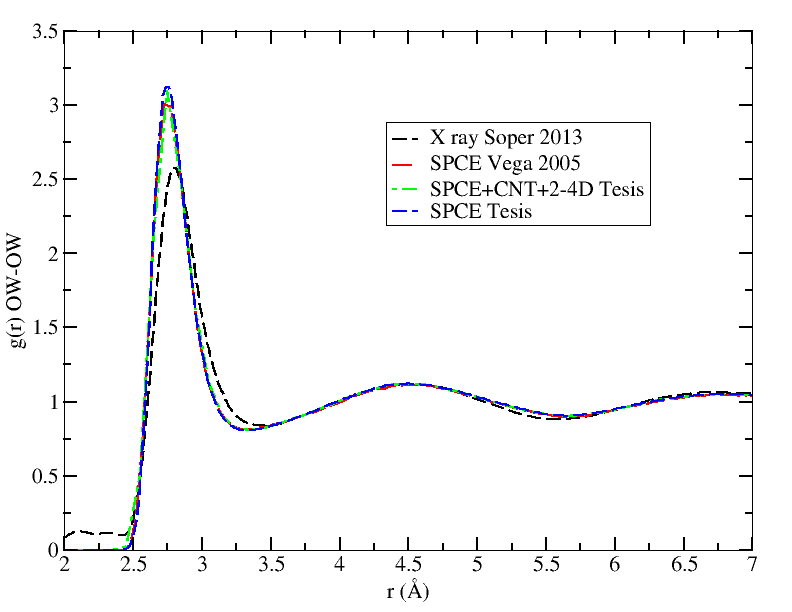
\includegraphics[width=0.7\textwidth,keepaspectratio=true]{resultados/gOOcartel.png}
    \caption{Función de distribución radial O-O de agua a 1 bar: comparación entre resultados experimentales (Soper, 2013)4, simulación de agua SPCE a 300 K (Vega, 2005)3, nuestra simulación de agua SPCE a 298.15 K, y función calculada en la mezcla de agua/herbicida a 298.15 K.}
    \label{fig:OO}
\end{figure}

En la figura \ref{fig:OO} se presenta una comparación de la función distribución radial del par oxigeno-oxigeno de agua: la linea negra corresponde a la función experimental obtenida por Soper \cite{Soper2013} a 298 K, las lineas de color roja y azul corresponden a funciones obtenidas en simulacion de agua pura de Vega \cite{vega2005} a 300 K y de nosotros a 298.15 K, respectivamente; la linea verde corresponde a la funcion obtenida en la mezcla presentada en este trabajo. Observamos un acuerdo entre funciones de distribución radial de simulación, igualmente la diferencia en la función obtenida por Soper en comparación con las otras era lo esperado. Por lo tanto, el agua sigue manteniendo la misma estructura ya sea en simulaciones de agua pura o en la mezcla de este trabajo.\\
% En la figura \ref{fig:24D_CNT_298_15_atom_atom} comparamos diferentes funciones de distribución radial a 298.25 K que se caracterizan como: carbono del nanotubo - átomo de 2,4-D. La función Cl(2,4-D)-C(CNT) y C(2,4-D)-C(CNT) tienen una distribución similar con dos máximos en aproximadamente $4.3<r1<4.5$ y $10.8<r2<11$ angstroms(\AA); y los pares  H(2,4-D)-C(CNT) y O(2,4-D)-C(CNT) tienen similares máximos con dos máximos en $r=5$ y $r=10.62$ \AA. Además, se puede observar que el hidrógeno de 2,4-D se encuentra mas cercano al carbón del nanotubo en $r\sim 2.3$\AA y el mas probable de los átomos en ser encontrado es el carbono de 2,4-D dado otro carbono en $r\sim 4.5$. \\

\newpage

\begin{figure}[!hbt]
    \centering
    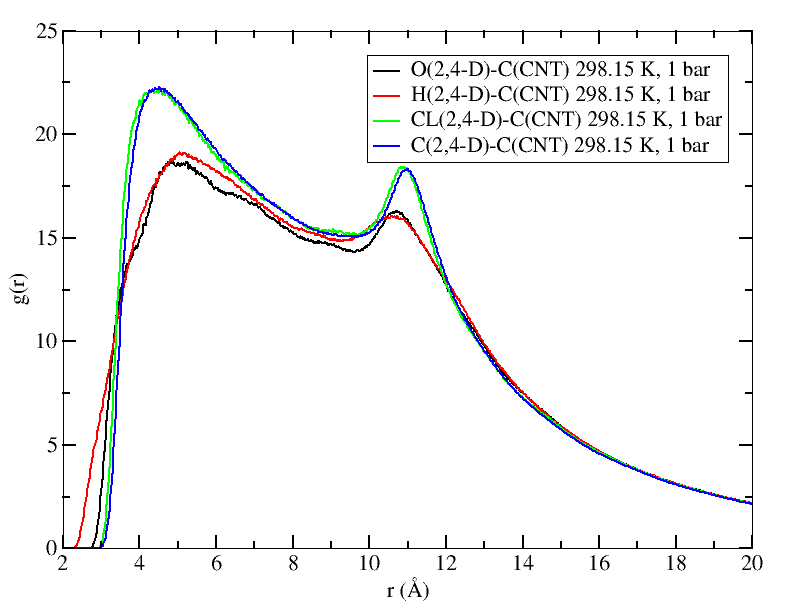
\includegraphics[width=0.6\textwidth,keepaspectratio=true]{resultados/gr_24D_CNT_298_15_atom_atom.png}
    \caption{Funciones de distribución radial átomo-átomo entre el C del nanotubo y átomos O, H, CL y C del 2,4-D a 298.15 K y 1 bar.}
    \label{fig:24D_CNT_298_15_atom_atom}
\end{figure}

En la figura \ref{fig:24D_CNT_298_15_atom_atom} se compararon diferentes funciones de distribución radial a 298.25 K del tipo átomo-átomo. La curva azul y verde corresponden a las funciones carbono del nanotubo-carbono de 2,4-D y carbono del nanotubo-cloro de 2,4-D respectivamente, entre estas funciones observamos que son similares con dos máximos en la distribución, $\sim 4.3$ \AA\  y $\sim 11$ \AA. La curva roja corresponde al par carbono del nanotubo-hidrógeno de 2,4-D, esta función comienza en $\sim 2$ \AA\  y el primer máximo se encuentra en $\sim 5$ \AA; y la curva negra corresponde a la función carbono del nanotubo-oxígeno de 2,4-D con un máximo alrededor de $\sim 5$ \AA. Observamos que la mayor concentración de moléculas alrededor del nanotubo esta entre el rango de $\sim 4.3$ \AA\  y $\sim 5$ \AA, donde el hidrógeno de 2,4-D es el mas cercano al nanotubo como las gráficas lo indican.

\newpage

\section{Número de coordinación}

\begin{figure}[!ht]
\begin{subfigure}{.5\textwidth}
  \centering
  % include first image
  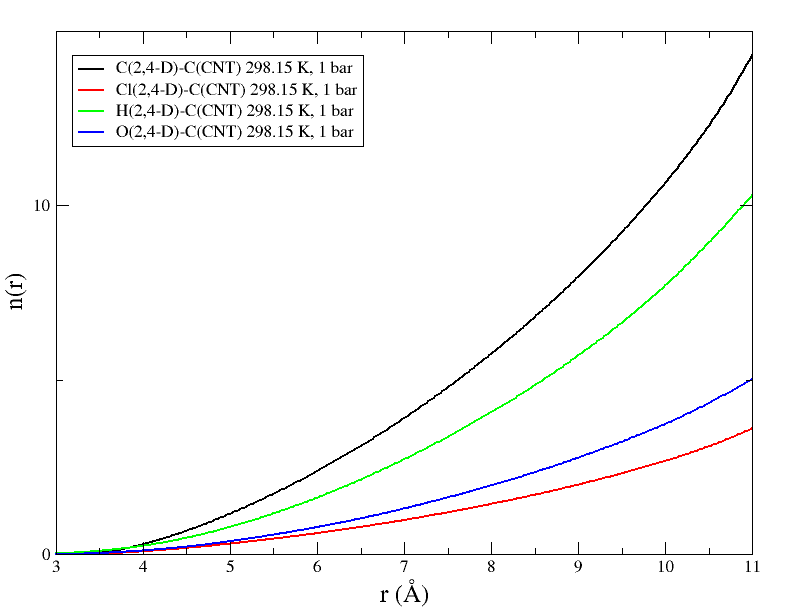
\includegraphics[width=1\linewidth]{resultados/gr_24D_CNT_298_15_atom_atom_cn_alt.png}  
  \caption{Número de coordinación de la figura \ref{fig:24D_CNT_298_15_atom_atom}.}
  \label{fig:24D_CNT_298_15_atom_atom_cn}
\end{subfigure}
\begin{subfigure}{.5\textwidth}
  \centering
  % include second image
  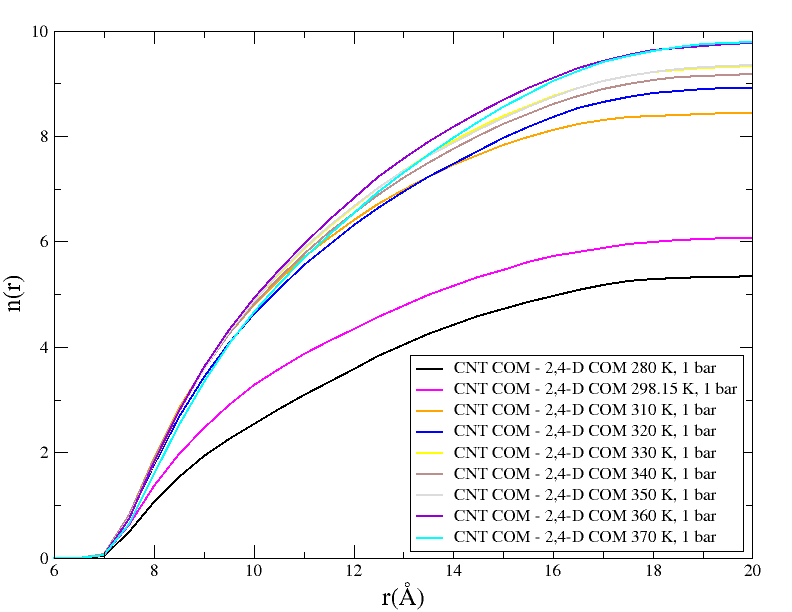
\includegraphics[width=1\linewidth]{resultados/cmnt_cmd_alltemp.png}  
  \caption{Número de coordinación de la función de distribución radial de centros de masa del nanotubo y 2,4-D en el rango de temperaturas 280-370 K.}
  \label{fig:24D_CNT_alltemp_CM-CM_cn}
\end{subfigure}
\caption{Números de coordinación}
\label{fig:24D_CNT_298_15_alltemp_atom_atom_cn}
\end{figure}

La figura \ref{fig:24D_CNT_298_15_atom_atom_cn} es el número de coordinación de la figura \ref{fig:24D_CNT_298_15_atom_atom}, se observa que a la distancia $\sim 5$ \AA\ hay $\sim 1$ átomo de hidrógeno y de carbono en promedio. En el caso de figura \ref{fig:24D_CNT_alltemp_CM-CM_cn} hay dos observaciones importantes, el número de moléculas alrededor del centro de masa del nanotubo aumentan con la temperatura y a 12 \AA\  del centro de masa del nanotubo se encuentran de 3 a 7 moléculas 2,4-D según la temperatura a la que se encuentra el sistema. En las figuras \ref{fig:24DCOM} y \ref{fig:CNTCOM} se observan los centros de masa de la molécula 2,4-D y el nanotubo de carbono respectivamente.\\

\begin{figure}[!h]
    \centering
    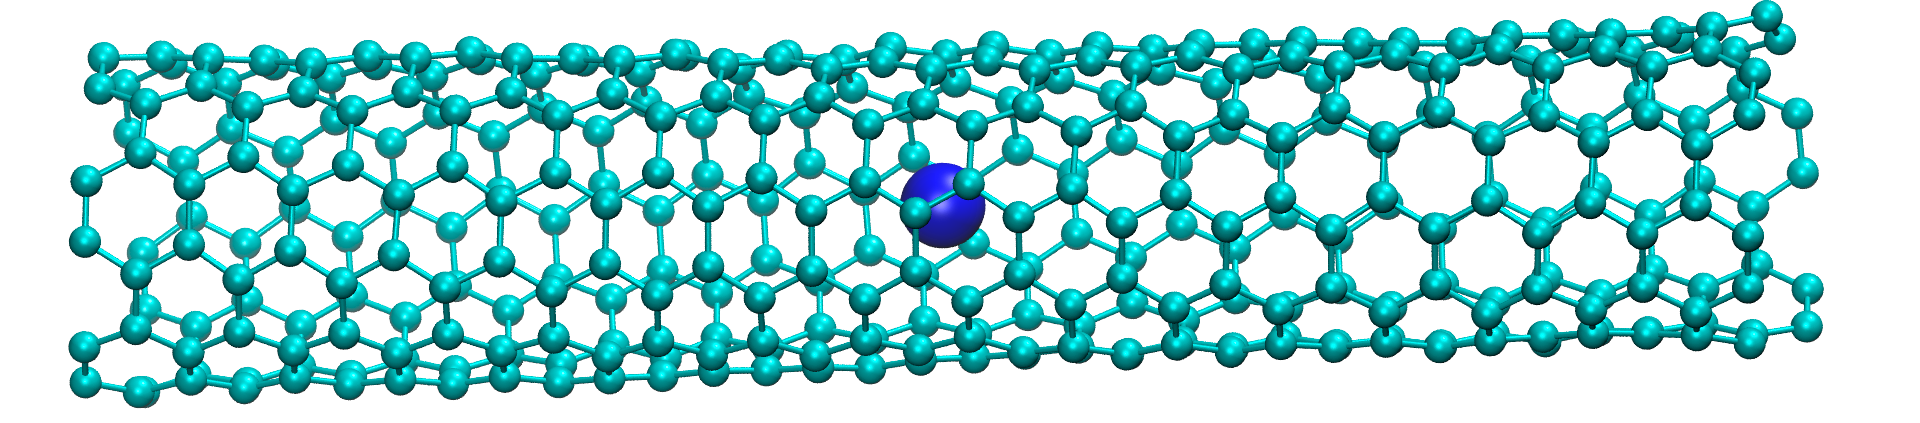
\includegraphics[width=.9\textwidth,keepaspectratio=true]{resultados/CNTCOM.png}
    \caption{Centro de masa del nanotubo de carbono (6,5),  presentado en este trabajo y representado por la esfera azul.}
    \label{fig:CNTCOM}
\end{figure}

\begin{figure}[!h]
    \centering
    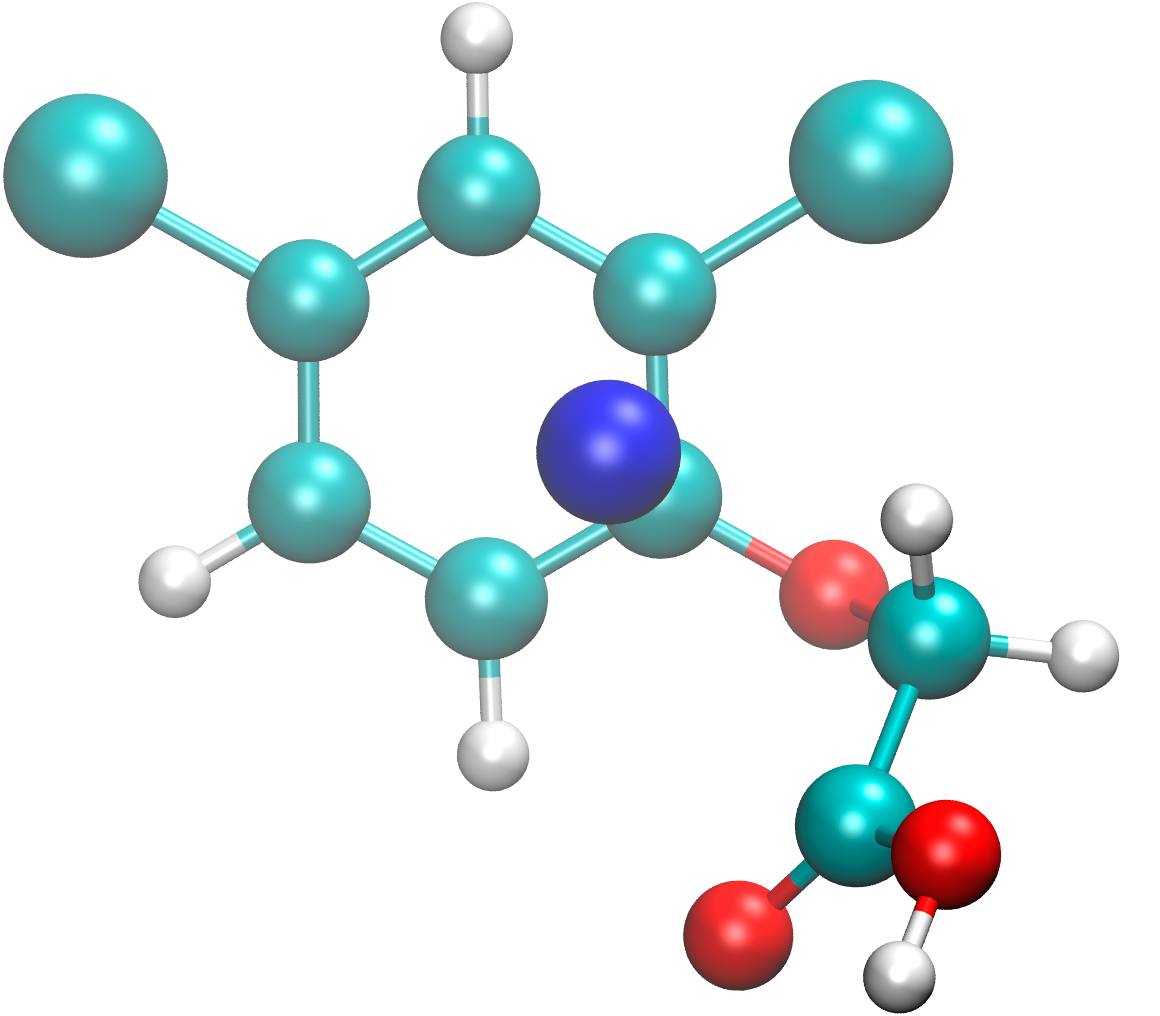
\includegraphics[width=.5\textwidth,keepaspectratio=true]{resultados/24DCOM.png}
    \caption{Centro de masa de la molécula de 2,4-D,  presentado en este trabajo y representado por la esfera azul.}
    \label{fig:24DCOM}
\end{figure}

Todas las funciones indican una cercanía y un interacción adsorbente entre el nanotubo de carbono y la molécula del herbicida. Esto se observa en todos los sistemas visualmente, por ejemplo, en la figura \ref{fig:Conffinal370}. 

% -------------------------------------------------------------------
% Funciones g(r)  [átomo A - átomo B]
% -------------------------------------------------------------------
% agua-agua:  g_OO,  g_OH,  g_HH   en funcion de la T (275 - 370 K) 
% agua-42D:   g_(OW-OD), g_(HW-HD), g_(OW-ClD), g_(HW-ClD), g_(OW-HD)
% agua-CNT:  g_(OW-C),  g_(HW-C)

% 42D-CNT:  g_(OD-C),  g_(HD-C),  g_(ClD-C),  g_(CD-C)
% 42D-42D:   g_(OD-OD),  g_(HD-HD),  g_(ClD-ClD),  g_(CD-CD),  g_(ClD-HD),  g_(OD-HD)

% CNT-CNT:   g_(C-C)
% ------------------------------------------------------------------------
% Funciones g(r)  [cm M - cm N]
% ------------------------------------------------------------------------
% CNT-42D:   g_(cm CNT - cm D),  g_(cm tapa CNT - cm D)

% ------------------------------------------------------------------------ 
% Funciones g(r)  [cm M -  átomo B]
% ------------------------------------------------------------------------
% CNT-42D:  g_(cm NT - ClD),  g_(cm NT - HD),  g_(cm NT - OD),  g_(cm NT - Cl1D), g_(cm NT - OD)
% CNT-agua:  g_(cm NT - OW),  g_(cm NT - HW)


\chapter{Conclusión}
Texto
\begin{figure}[!h]
\centering

\includegraphics[width=.2\textwidth,keepaspectratio=true]{escudo-2}
\end{figure}

mas texto Loren itsu
\[ \vec E = \vec \nabla \cdot \vec \nabla \vec r \times \vec A
\]

\appendix % A partir de esta línea van los apéndices. Quitar si no habrá apéndices
\chapter{Modelo del sistema solvatado}\label{chapter:apendicea}

\textcolor{red}{Encabezados de tablas}

% \section{Parámetros de los modelos}

% \subsection{Modelo de agua}

% El modelo de agua elegido para estas simulaciones fue el modelo SPC/E(punto simple punto de carga extendido) rígido, tiene cargas situadas en los tres átomos y la interacción Lennard-Jones con otras moléculas esta situada en el oxígeno. La figura (\ref{fig:SPCE}) es una visualización de la molécula y la tabla (\ref{SPCEpar}) son los parámetros del modelo.

% \begin{figure}[!h]
%     \centering
%     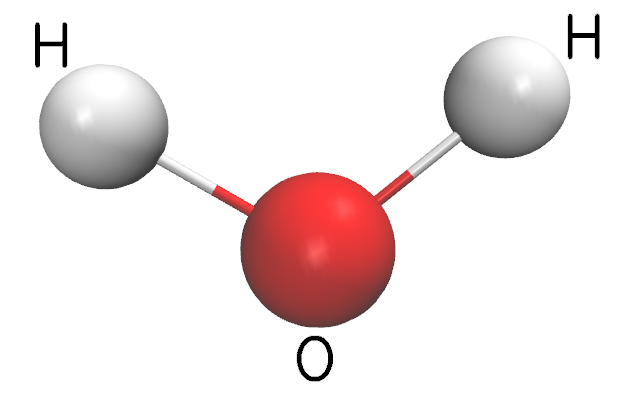
\includegraphics[width=.9\textwidth,keepaspectratio=true]{SPCE.png}
%     \caption{Molécula de agua}
%     \label{fig:SPCE}
% \end{figure}

% \begin{table}[h!]
%     \centering

%     \begin{tabular}{ |p{1cm}|p{4cm}|  }
%     \hline
%     $\sigma$  & 3.166 \AA \\
%     $\epsilon$& 0.650 KJ $mol^{-1}$ \\
%     $r_{OH}$  & 1.000 \AA \\
%     $\angle_{HOH}$&109.47 deg \\
%     $q_{O}$   & -0.8476 e \\
%     $q_{H}$   & 0.4238 e \\
%     \hline
%     \end{tabular}
%     \caption{Parámetros del modelo SPCE}
%     \label{SPCEpar}
% \end{table}

% \newpage

El sistema se compone de un nanotubo de carbono (6,5) y 10 moléculas de 2,4D. La siguientes tablas contienen los parámetros de simulación.

\begin{table}[!h]
    \centering
    \begin{tabular}{|l|c|l|c|}
    \hline
    Parámetro & valor & Parámeto & valor \\
    \hline
    $\epsilon_{cc}$ & 0.4058kJ/mol & $q_{o}$   & -0.8476e \\
    $\epsilon_{oo}$ & 0.6502kJ/mol &  $q_H$    & 0.4238e \\
    $\epsilon_{co}$ & 0.5137kJ/mol & $K^b_{CC}$& 3.2236X$10^6$ $\frac{kJ}{molnm^4}$\\
    $\sigma_{cc}$   & 3.361        & $b_{ij}$  & 1.42 \AA\\
    $\sigma_{oo}$   & 3.166        & $K^{\theta}_{CCC}$& 560 $\frac{kJ}{mol}$ \\
    $\sigma_{co}$   & 3.262        & $\theta^0_{ijk}$  & $120^{\circ}$ \\
    $r_{OH}$        & 1 \AA        & $k^{\phi}_{CCCC}$ & 5.86 $\frac{kJ}{mol}$ \\
    $\theta_{HOH}$  & $109.47^{\circ}$ & $\phi_s$         & $180^{\circ}$ \\
    \hline
    \end{tabular}
    \caption{Parámetros del modelo SPCE de agua y del nanotubo de carbono. \cite{meng2008}}
    \label{tab:cnth2oparameters}
\end{table}

\begin{figure}[!h]
    \centering
    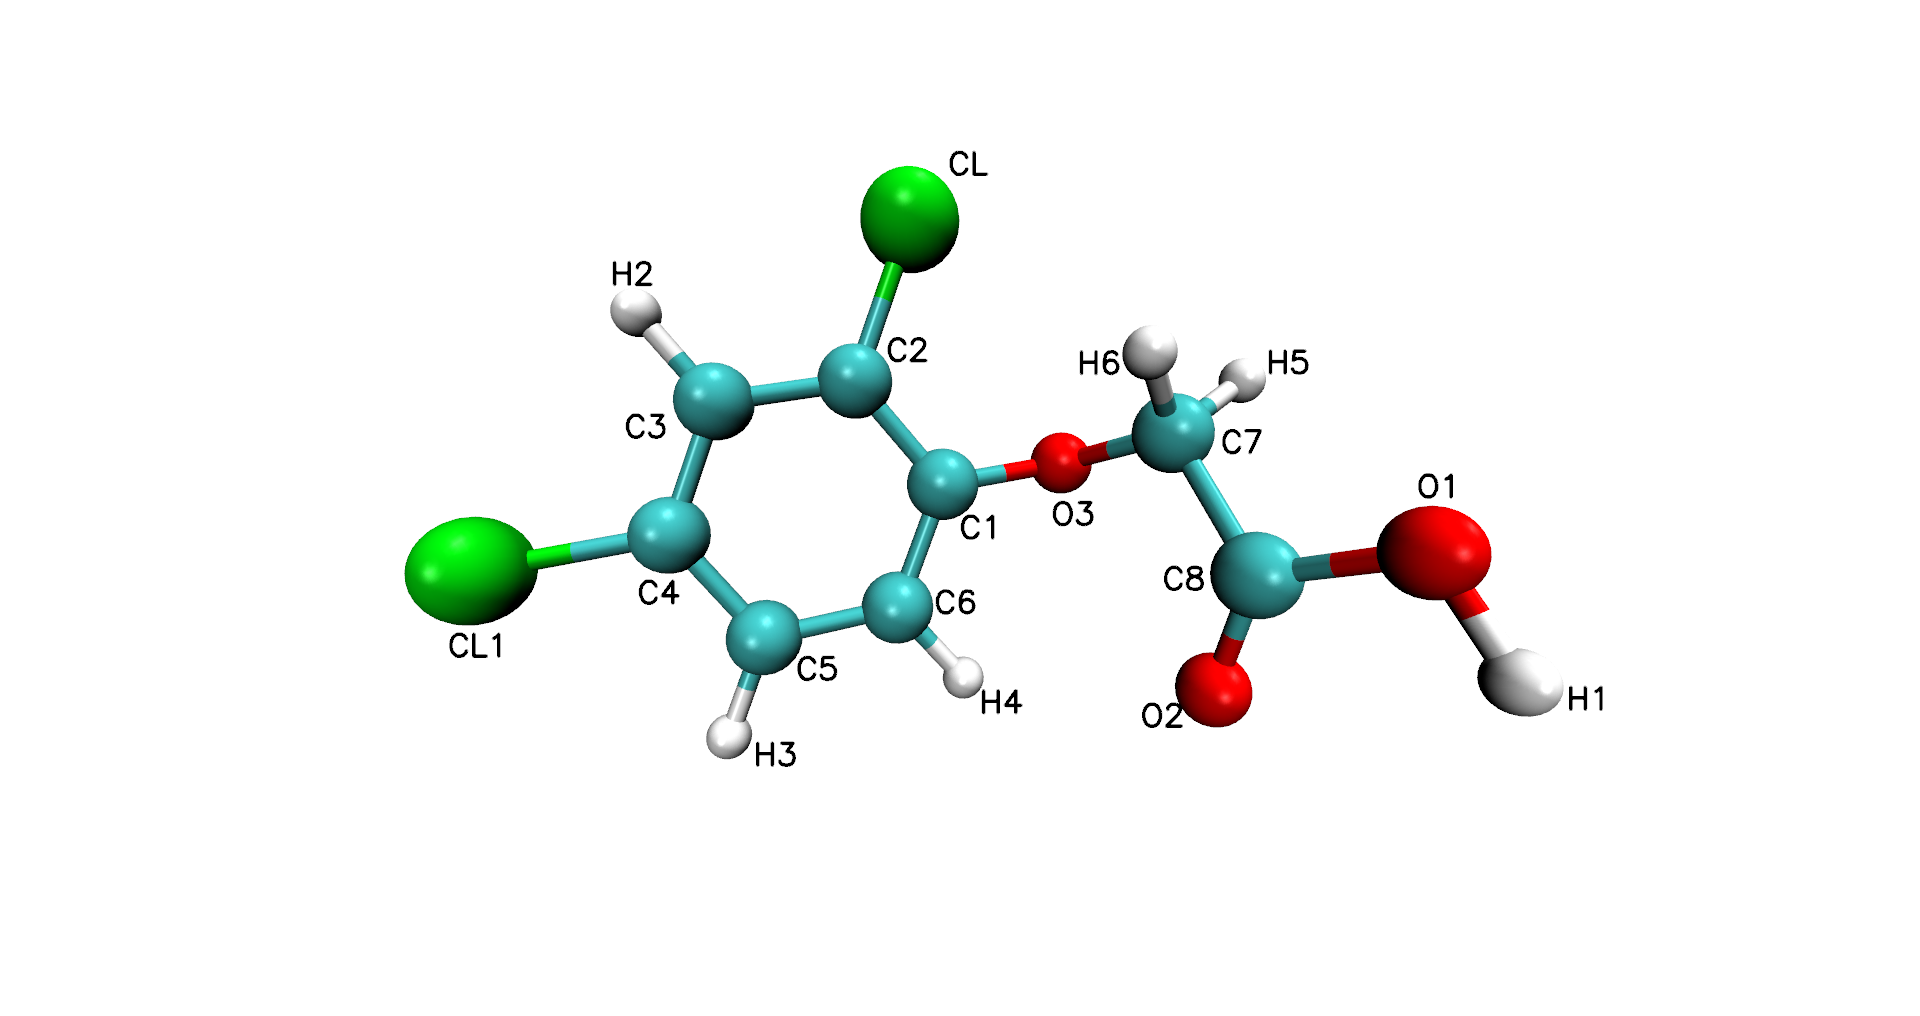
\includegraphics[width=.9\textwidth,keepaspectratio=true]{figura_nueva_tarea.png}
    \caption{Molécula 2,4-D}
    \label{fig:24Dfigure}
\end{figure}

\newpage

% \begin{table}[!h]
% \caption{\label{tab:cnth2oparameters}
% Parámetros del agua rígida y el nanotubo de carbono. \cite{meng2008}}
% \centering
% \begin{tabular}{| c | c || c | c |}
% % &$r_c$ (\AA)&
% % &$r_c$ (\AA)\\
% \hline
% \large{$\epsilon_{cc}$}\footnotemark[1] & 0.4058 kJ/mol & {\large q}_O & -0.8476 e \\
% \large{$\epsilon_{oo}$}\footnotemark[1]& 0.6502 kJ/mol &{\large q}_H& 0.4238 e \\
% \large{$\epsilon_{co}$}\footnotemark[1]& 0.5137 kJ/mol &{\large K}^b_{CC}& 3.2236X10^6 $\frac{kJ}{mol\ nm^4}$\\
% \large{$\sigma_{cc}$}\footnotemark[1]&   3.361         &{\large b}_{ij}& 1.42 \AA\\
% \large{$\sigma_{oo}$}\footnotemark[1]&   3.166         &{\large K}^{$\theta$}_{CCC}& $560 \frac{kJ}{mol}$ \\
% \large{$\sigma_{co}$}\footnotemark[1]&   3.262         &{\large $\theta$}^0_{ijk}& $120^{\circ}$ \\
% {\large r}_{OH}& 1 \AA                                 &{\large k}^{$\phi$}_{CCCC}& 5.86 $\frac{kJ}{mol}$ \\
% {\large $\theta$}_{HOH}& 109.47^{\circ}                &{\large $\phi$}_s& $180^{\circ}$ \\
% \hline
% \end{tabular}
% \footnotetext[1]{Provided in GROMACS}
% \end{table}

% [ moleculetype ]
% ; Name   nrexcl
% SAYK     3
% [ atoms ]
% ;  nr  type  resnr  resid  atom  cgnr  charge    mass
%     1 CLAro    1    SAYK    CL1    1   -0.095  35.4530
%     2  CAro    1    SAYK     C4    2   -0.125  12.0110
%     3  CAro    1    SAYK     C3    3    0.070  12.0110
%     4    HC    1    SAYK     H2    4    0.116   1.0080
%     5  CAro    1    SAYK     C2    5   -0.185  12.0110
%     6 CLAro    1    SAYK     CL    6   -0.070  35.4530
%     7  CAro    1    SAYK     C1    7    0.491  12.0110
%     8  CAro    1    SAYK     C6    8   -0.375  12.0110
%     9    HC    1    SAYK     H4    9    0.212   1.0080
%   10  CAro    1    SAYK     C5   10    0.037  12.0110
%   11    HC    1    SAYK     H3   11    0.130   1.0080
%   12    OE    1    SAYK     O3   12   -0.431  15.9994
%   13  CPos    1    SAYK     C7   13    0.038  12.0110
%   14    HC    1    SAYK     H5   14    0.099   1.0080
%   15    HC    1    SAYK     H6   15    0.099   1.0080
%   16  CPos    1    SAYK     C8   16    0.683  12.0110
%   17 OEOpt    1    SAYK     O2   17   -0.549  15.9994
%   18    OA    1    SAYK     O1   18   -0.610  15.9994
%   19  HS14    1    SAYK     H1   19    0.465   1.0080
% ; total charge of the molecule:   0.000
% [ bonds ]
% ;  ai   aj  funct   c0         c1
%     1    2    2   0.1760   1.4366e+06
%     2    3    2   0.1390   8.6600e+06
%     2   10    2   0.1390   8.6600e+06
%     3    4    2   0.1090   1.2300e+07
%     3    5    2   0.1390   8.6600e+06
%     5    6    2   0.1760   1.4366e+06
%     5    7    2   0.1400   8.5400e+06
%     7    8    2   0.1390   8.6600e+06
%     7   12    2   0.1380   1.1000e+07
%     8    9    2   0.1090   1.2300e+07
%     8   10    2   0.1390   8.6600e+06
%   10   11    2   0.1090   1.2300e+07
%   12   13    2   0.1430   8.1800e+06
%   13   14    2   0.1090   1.2300e+07
%   13   15    2   0.1090   1.2300e+07
%   13   16    2   0.1530   7.1500e+06
%   16   17    2   0.1210   1.2977e+07
%   16   18    2   0.1350   1.0300e+07
%   18   19    2   0.0983   9.8314e+06
% [ pairs ]
% ;  ai   aj  funct  ;  all 1-4 pairs but the ones excluded in GROMOS itp
%     1    4    1
%     1    5    1
%     1    8    1
%     1   11    1
%     2    6    1
%     2    9    1
%     3   11    1
%     3   12    1
%     4    6    1
%     4    7    1
%     4   10    1
%     5    9    1
%     5   13    1
%     6    8    1
%     6   12    1
%     7   11    1
%     7   14    1
%     7   15    1
%     7   16    1
%     8   13    1
%     9   11    1
%     9   12    1
%   10   12    1
%   12   17    1
%   12   18    1
%   13   19    1
%   14   17    1
%   14   18    1
%   15   17    1
%   15   18    1
%   17   19    1
% [ angles ]
% ;  ai   aj   ak  funct   angle     fc
%     1    2    3    2    120.00   560.00
%     1    2   10    2    120.00   560.00
%     3    2   10    2    120.00   560.00
%     2    3    4    2    120.00   505.00
%     2    3    5    2    120.00   560.00
%     4    3    5    2    120.00   505.00
%     3    5    6    2    120.00   560.00
%     3    5    7    2    120.00   560.00
%     6    5    7    2    120.00   560.00
%     5    7    8    2    120.00   560.00
%     5    7   12    2    121.00   685.00
%     8    7   12    2    120.00   560.00
%     7    8    9    2    120.00   505.00
%     7    8   10    2    120.00   560.00
%     9    8   10    2    120.00   505.00
%     2   10    8    2    120.00   560.00
%     2   10   11    2    120.00   505.00
%     8   10   11    2    120.00   505.00
%     7   12   13    2    119.00  2211.40
%   12   13   14    2    106.75   503.00
%   12   13   15    2    106.75   503.00
%   12   13   16    2    111.00   530.00
%   14   13   15    2    107.57   484.00
%   14   13   16    2    109.60   450.00
%   15   13   16    2    109.60   450.00
%   13   16   17    2    126.00   640.00
%   13   16   18    2    109.50   520.00
%   17   16   18    2    124.00   730.00
%   16   18   19    2    109.50   450.00
% [ dihedrals ]
% ; GROMOS improper dihedrals
% ;  ai   aj   ak   al  funct   angle     fc
%     7    5    8   12    2      0.00   167.36
%     5    3    6    7    2      0.00   167.36
%     3    2    4    5    2      0.00   167.36
%     2    1    3   10    2      0.00   167.36
%   10    2    8   11    2      0.00   167.36
%     8    7    9   10    2      0.00   167.36
%   16   13   17   18    2      0.00   167.36
% [ dihedrals ]
% ;  ai   aj   ak   al  funct    ph0      cp     mult
%     2    3    5    7    1    180.00    41.80    2
%     3    2   10    8    1    180.00    41.80    2
%     3    5    7    8    1    180.00    41.80    2
%     5    7    8   10    1    180.00    41.80    2
%     5    7   12   13    1      0.00     0.42    2
%     7    8   10    2    1    180.00    41.80    2
%     7   12   13   16    1      0.00     1.26    3
%   10    2    3    5    1    180.00    41.80    2
%   12   13   16   18    1    180.00     1.00    6
%   17   16   18   19    1    180.00     7.11    2
% [ exclusions ]
% ;  ai   aj  funct  ;  GROMOS 1-4 exclusions
%     2    7
%     3    8
%     5   10

\begin{table}[!h]
    \centering
    \begin{tabular}{|c|c|}
    \hline
    \large{$q_{\text{molécula}}$} & q(e) \\
    \hline
    \large{$q_{CL}$} & -0.070 e \\
    \large{$q_{CL1}$} & -0.095 e \\
    \large{$q_{C1}$} & 0.491 e \\
    \large{$q_{C2}$} & -0.185 e \\
    \large{$q_{C3}$} & 0.070 e \\
    \large{$q_{C4}$} & -0.125 e \\
    \large{$q_{C5}$} & 0.037 e \\
    \large{$q_{C6}$} & -0.375 e \\
    \large{$q_{C7}$} & 0.038 e \\
    \large{$q_{C8}$} & 0.683 e \\
    \large{$q_{H1}$} & 0.465 e \\
    \large{$q_{H2}$} & 0.116 e \\
    \large{$q_{H3}$} & 0.130 e \\
    \large{$q_{H4}$} & 0.212 e \\
    \large{$q_{H5}$} & 0.099 e \\
    \large{$q_{H6}$} & 0.099 e \\
    \large{$q_{O1}$} & -0.610 e \\
    \large{$q_{O2}$} & -0.549 e \\
    \large{$q_{O3}$} & -0.431 e \\
    \hline
    \end{tabular}
    \caption{Tabla de cargas en 2,4-D}
    \label{tab:cargas24D}
\end{table}


\begin{table}[!h]
    \centering
    \begin{tabular}{|c|c|}
    \hline
    $K^b_{ij}$ $b_{ij}$   & ($\frac{kJ}{molnm^4}$) (\AA)\\
    % \multicolumn{2}{|c|}{$K^b_{ij}$ ($\frac{kJ}{molnm^4}$) $b_{ij}$ (\AA)}\\
    \hline
    $K^b_{C1-C2}\ b_{C1-C2}$   & 8.5400X$10^6$ 1.400\\
    $K^b_{C2-C3}\ b_{C2-C3}$   & 8.6600X$10^6$ 1.390\\
    $K^b_{C3-C4}\ b_{C3-C4}$   & 8.6600X$10^6$ 1.390\\
    $K^b_{C4-C5}\ b_{C4-C5}$   & 8.6600X$10^6$ 1.390\\
    $K^b_{C5-C6}\ b_{C5-C6}$   & 8.6600X$10^6$ 1.390\\
    $K^b_{C7-C8}\ b_{C7-C8}$   & 7.1500X$10^6$ 1.530\\
    $K^b_{C1-C6}\ b_{C1-C6}$   & 8.6600X$10^6$ 1.390\\
    $K^b_{CL1-C4}\ b_{CL1-C4}$ & 1.4366X$10^6$ 1.760\\
    $K^b_{C2-CL}\ b_{C2-CL}$   & 1.4366X$10^6$ 1.760\\
    $K^b_{C5-H3}\ b_{C5-H3}$   & 1.2300X$10^7$ 1.090\\
    $K^b_{C6-H4}\ b_{C6-H4}$   & 1.2300X$10^7$ 1.090\\
    $K^b_{C3-H2}\ b_{C3-H2}$   & 1.2300X$10^7$ 1.090\\
    $K^b_{C1-O3}\ b_{C1-O3}$   & 1.1000X$10^7$ 1.380\\
    $K^b_{O3-C7}\ b_{O3-C7}$   & 8.1800X$10^6$ 1.430\\
    $K^b_{H5-C7}\ b_{H5-C7}$   & 1.2300X$10^7$ 1.090\\
    $K^b_{H6-C7}\ b_{H6-C7}$   & 1.2300X$10^7$ 1.090\\
    $K^b_{O2-C8}\ b_{O2-C8}$   & 1.2977X$10^7$ 1.210\\
    $K^b_{O-C8} \ b_{O1-C8}$   & 1.0300X$10^7$ 1.210\\
    $K^b_{O1-H1}\ b_{O1-H1}$   & 9.8314X$10^6$ 0.983\\
    \hline
    \end{tabular}
    \caption{Tabla de parámetros del potencial de enlace de 2,4-D}
    \label{tab:enlace24D}
\end{table}



\begin{table}[!h]
    \centering
    \begin{tabular}{|c|c|}
    \hline
    $K^{\theta}_{ijk}$ $\theta^0_{ijk}$& $\frac{kJ}{mol}$\quad $^{\circ}$\\
    \hline
    $K^{\theta}_{C3-C4-CL1} \theta^0_{C3-C4-CL1}$& 560 120\\
    $K^{\theta}_{C4-C5-CL1} \theta^0_{C4-C5-CL1}$& 560 120\\
    $K^{\theta}_{C3-C4-C5} \theta^0_{C3-C4-C5}$& 560 120\\
    $K^{\theta}_{C2-C3-C4} \theta^0_{C2-C3-C4}$& 560 120\\
    $K^{\theta}_{C2-C3-CL} \theta^0_{C2-C3-CL}$& 560 120\\
    $K^{\theta}_{C1-C2-C3} \theta^0_{C1-C2-C3}$& 560 120\\
    $K^{\theta}_{C1-C2-CL} \theta^0_{C1-C2-CL}$& 560 120\\
    $K^{\theta}_{C1-C2-C6} \theta^0_{C1-C2-C6}$& 560 120\\
    $K^{\theta}_{C1-C6-O3} \theta^0_{C1-C6-O3}$& 560 120\\
    $K^{\theta}_{C1-C6-C5} \theta^0_{C1-C6-C5}$& 560 120\\
    $K^{\theta}_{C4-C5-C6} \theta^0_{C4-C5-C6}$& 560 120\\

    $K^{\theta}_{C3-C4-H2} \theta^0_{C3-C4-H2}$& 505 120\\
    $K^{\theta}_{C2-C3-H2} \theta^0_{C2-C3-H2}$& 505 120\\
    $K^{\theta}_{C1-C6-H4} \theta^0_{C1-C6-H4}$& 505 120\\
    $K^{\theta}_{C5-C6-H4} \theta^0_{C5-C6-H4}$& 505 120\\
    $K^{\theta}_{C4-C5-H3} \theta^0_{C4-C5-H3}$& 505 120\\
    $K^{\theta}_{C5-C6-H3} \theta^0_{C5-C6-H3}$& 505 120\\
    
    $K^{\theta}_{C7-C8-H5} \theta^0_{C7-C8-H5}$& 450 109.60\\
    $K^{\theta}_{C7-C8-H6} \theta^0_{C7-C8-H6}$& 450 109.60\\
    $K^{\theta}_{C8-O1-H1} \theta^0_{C8-O1-H1}$& 450 109.50\\
    $K^{\theta}_{C7-C8-O1} \theta^0_{C7-C8-O1}$& 520 109.50\\
    
    $K^{\theta}_{C7-H5-H6} \theta^0_{C7-H5-H6}$& 484 107.57\\
    $K^{\theta}_{O3-C7-H5} \theta^0_{O3-C7-H5}$& 503 106.75\\
    $K^{\theta}_{O3-C7-H6} \theta^0_{O3-C7-H6}$& 503 106.75\\
    $K^{\theta}_{O3-C7-C8} \theta^0_{O3-C7-C8}$& 530 111\\
    $K^{\theta}_{C7-C8-O2} \theta^0_{C7-C8-O2}$& 640 126\\
    $K^{\theta}_{C1-C2-O3} \theta^0_{C1-C2-O3}$& 685 121\\
    $K^{\theta}_{C8-O2-O1} \theta^0_{C8-O2-O1}$& 730 124\\
    $K^{\theta}_{C1-C7-O3} \theta^0_{C1-C7-O3}$& 2211.40 119\\
    \hline
    \end{tabular}
    \caption{Tabla de parametros de ángulos de 2,4-D}
    \label{tab:angulos24D}
\end{table}

\begin{table}[!h]
    \centering
    \begin{tabular}{|c|c|}
    \hline
    $k^{\xi}_{ijkl}$ $\xi^{0}_{ijkl}$ & $\frac{kJ}{molrad^2}$\quad $^{\circ}$ \\
    \hline
    $k^{\xi}_{C1-C2-C6-O3}$ $\xi_{0}$ & 167.36 0\\
    $k^{\xi}_{C1-C2-C3-CL}$ $\xi_{0}$ & 167.36 0\\
    $k^{\xi}_{C2-C3-C4-H2}$ $\xi_{0}$ & 167.36 0\\
    $k^{\xi}_{C3-C4-C5-CL1}$ $\xi_{0}$ & 167.36 0 \\
    $k^{\xi}_{C4-C5-C6-H3}$ $\xi_{0}$ & 167.36 0\\
    $k^{\xi}_{C1-C5-C6-H4}$ $\xi_{0}$ & 167.36 0\\
    $k^{\xi}_{C7-C8-O1-O2}$ $\xi_{0}$ & 167.36 0\\
    \hline
    $k^{\phi}_{ijkl}$ $\phi^s_{ijkl}$ & $\frac{kJ}{mol}$\quad $^{\circ}$\\
    \hline
    $k^{\phi}_{C1-C2-C3-C4}$ $\phi_s$ & 41.80 180\\
    $k^{\phi}_{C3-C4-C5-C6}$ $\phi_s$ & 41.80 180\\
    $k^{\phi}_{C1-C2-C3-C6}$ $\phi_s$ & 41.80 180\\
    $k^{\phi}_{C1-C2-C5-C6}$ $\phi_s$ & 41.80 180\\
    $k^{\phi}_{C1-C4-C5-C6}$ $\phi_s$ & 41.80 180\\
    $k^{\phi}_{C2-C3-C4-C5}$ $\phi_s$ & 41.80 180\\
    $k^{\phi}_{C7-C8-O1-O3}$ $\phi_s$ n & 1.00 180 6\\
    $k^{\phi}_{C8-O1-O2-H1}$ $\phi_s$ n & 7.11 180 2\\
    $k^{\phi}_{C1-C2-O3-C7}$ $\phi_s$ n & 0.42 0 2\\
    $k^{\phi}_{C1-C7-C8-O3}$ $\phi_s$ n & 1.26 0 3\\
    \hline
    \end{tabular}
    \caption{Tabla de parámetros del potencial de ángulos diedros de 2,4-D}
    \label{tab:angulosdih24D}
\end{table}

\newpage
%               c6              c12                sigma                 epsilon
% C    CLAro      1  0.003974417     6.381584e-06       0.3421967204782815    0.6188115086273643
% C     CAro      1  0.002340624     4.690642e-06      sigma: 0.3550722828524636, epsilon: 0.29199205084165447
% HC	C	      1	4.450960E-04	2.733060E-07      sigma: 0.2915407359639445, epsilon: 0.18121670327032705
% C	OE	          1	2.300953E-03	2.444200E-06          sigma: 0.31942690878969837, epsilon: 0.541525315871144
% C     CPos      1  0.0021771       2.222e-06         sigma: 0.31730550936068447, epsilon: 0.5332768238073807
% C    OEOpt      1  0.00268896      4.85507e-06       sigma: 0.34895427699812803, epsilon: 0.37231728284041216
% C     HS14      1  0               0           
% C	OA	          1	2.300953E-03	2.444200E-06          sigma: 0.31942690878969837, epsilon: 0.541525315871144

% OA    CLAro     1  0.003907054     3.1592e-06       sigma: 0.3052258307853132, epsilon: 1.2079854835809698
% OW    CLAro     1  0.004202794     4.661256e-06     sigma: 0.3217319135230157, epsilon: 0.9473561099431141
% HS14    CLAro   1  0               0
% CLAro    OEOpt  1  0.004565897     6.27532e-06   sigma: 0.33344045848470744, epsilon: 0.830531965485784
% CLAro     CAro  1  0.003974417     6.062792e-06  sigma: 0.3392864686204393, epsilon: 0.6513496789057335
% CLAro     CPos  1  0.00369675      2.872e-06     sigma: 0.3031987401164613, epsilon: 1.1895857035602366
% OE    CLAro     1  0.003907054     3.231e-06        sigma: 0.30637119042109173, epsilon: 1.181141361723615
% HC    CLAro     1  0.00075578      3.53256e-07      sigma: 0.27857941708920847, epsilon: 0.4042418305704644

% OE     CAro     1  0.002300953     2.3221e-06       sigma: 0.3167103054468882, epsilon: 0.5699996456019336
% OA     CAro     1  0.002300953     2.3221e-06       sigma: 0.3167103054468882, epsilon: 0.5699996456019336
% OW     CAro     1  0.002475121     3.426153e-06     sigma: 0.33383744896554585, epsilon: 0.44701914688580746
% HC     CAro     1  0.000445096     2.59653e-07      sigma: 0.2890612938252534, epsilon: 0.19074538828359391
% HS14     CAro   1  0               0
% OEOpt     CAro  1  0.00268896      4.612535e-06  sigma: 0.34598655471395084, epsilon: 0.39189436403192596
% CAro     CPos   1  0.0021771       2.111e-06      sigma: 0.3146069477063536, epsilon: 0.56131743368072
% CAro     CAro   1  0.002340624     4.456321e-06   sigma: 0.3520525292750613, epsilon: 0.30734549359078933

% HC	OA	      1	4.375520E-04	1.353000E-07      sigma: 0.2600427123263571, epsilon: 0.3537541624242424
% HC	OE	      1	4.375520E-04	1.353000E-07      sigma: 0.2600427123263571, epsilon: 0.3537541624242424
% HC	OW	      1	4.706720E-04	1.996290E-07      sigma: 0.2741053705029336, epsilon: 0.2774297967529768
% HC     HS14     1  8.464e-05       1.5129e-08       sigma: 0.23734081428097492, epsilon: 0.1183807521977659
% HC    OEOpt     1  0.000511336     2.68755e-07      sigma: 0.28408067888820254, epsilon: 0.24321827026101842
% HC     CPos     1  0.000414        1.23e-07         sigma: 0.2583156954670584, epsilon: 0.34836585365853656
    
% OE     HS14     1  0               0     
% OE    OEOpt     1  0.002643385     2.4035e-06       sigma: 0.31125329012564956, epsilon: 0.7268030224906386
% OE     CPos     1  0.0021402       1.1e-06          sigma: 0.28302386291723314, epsilon: 1.0410127363636363
    
% OA     CPos     1  0.0021402       1.1e-06          sigma: 0.28302386291723314, epsilon: 1.0410127363636363
% OW     CPos     1  0.0023022       1.623e-06        sigma: 0.2983293017984591, epsilon: 0.8164086321626617
% HS14     CPos   1  0               0
% OEOpt     CPos  1  0.0025011       2.185e-06     sigma: 0.3091861733013462, epsilon: 0.7157324038901602

% OA    OEOpt     1  0.002643385     2.4035e-06       sigma: 0.31125329012564956, epsilon: 0.7268030224906386
% OW    OEOpt     1  0.002843473     3.546255e-06     sigma: 0.32808532768562954, epsilon: 0.5699913501517093
% HS14    OEOpt   1  0               0

% OA     HS14     1  0               0

% OW     HS14     1  0               0
% HS14     HS14   1  8.464e-05       1.5129e-08     sigma: 0.23734081428097492, epsilon: 0.1183807521977659

La tabla \ref{tab:lennardjonesall} muestran los parámetros Lennard-Jones para 2,4-D con el nanotubo del carbono, con agua y consigo misma. La lista \ref{tab:24Ditp} es el tipo de átomo dentro de GROMACS para cada átomo de 2,4-D en la figura \ref{fig:24Dfigure} descrito en el archivo itp.

\begin{table}[!h]
    \centering
    \begin{tabular}{|c|c|}
    \hline
    tipo & átomo\\
    \hline
   CLAro & CL1\\
    CAro &  C4\\
    CAro &  C3\\
      HC &  H2\\
    CAro &  C2\\
   CLAro &  CL\\
    CAro &  C1\\
    CAro &  C6\\
      HC &  H4\\
    CAro &  C5\\
      HC &  H3\\
      OE &  O3\\
    CPos &  C7\\
      HC &  H5\\
      HC &  H6\\
    CPos &  C8\\
   OEOpt &  O2\\
      OA &  O1\\
    HS14 &  H1\\
    \hline
    \end{tabular}
    \caption{Lista de átomos en el archivo .itp de 2,4-D}
    \label{tab:24Ditp}
\end{table}


\begin{table}[!h]
    \centering
    \begin{tabular}{|c|c|}
    \hline
        $a_1$ $a_2$ & $\sigma$(nm) $\epsilon$(kJ/mol) \\
        \hline
        C    CLAro      &     0.3421967204782815 0.6188115086273643\\
        C     CAro      &     0.3550722828524636 0.29199205084165447\\
        HC	C	        &     0.2915407359639445 0.18121670327032705\\
        C	OE	        &     0.31942690878969837 0.541525315871144\\
        C     CPos      &     0.31730550936068447 0.5332768238073807\\
        C    OEOpt      &     0.34895427699812803 0.37231728284041216\\
        C     HS14      &     0                   0\\
        C	OA	        &     0.31942690878969837 0.541525315871144\\
        OA    CLAro     &     0.3052258307853132 1.2079854835809698\\
        OW    CLAro     &     0.3217319135230157 0.9473561099431141\\
        HS14    CLAro   &     0                   0\\
        CLAro    OEOpt  &     0.33344045848470744 0.830531965485784\\
        CLAro     CAro  &     0.3392864686204393 0.6513496789057335\\
        CLAro     CPos  &     0.3031987401164613 1.1895857035602366\\
        OE    CLAro     &     0.30637119042109173 1.181141361723615\\
        HC    CLAro     &     0.27857941708920847 0.4042418305704644\\
        OE     CAro     &     0.3167103054468882 0.5699996456019336\\
        OA     CAro     &     0.3167103054468882 0.5699996456019336\\
        OW     CAro     &     0.33383744896554585 0.44701914688580746\\
        HC     CAro     &     0.2890612938252534 0.19074538828359391\\
        HS14     CAro   &     0                   0\\
        OEOpt     CAro  &     0.34598655471395084 0.39189436403192596\\
        CAro     CPos   &     0.3146069477063536 0.56131743368072\\
        CAro     CAro   &     0.3520525292750613 0.30734549359078933\\
        HC	OW	        &     0.2741053705029336 0.2774297967529768\\
        HC	OE	        &     0.2600427123263571 0.3537541624242424\\
        HC	OA	        &     0.2600427123263571 0.3537541624242424\\
        HC     HS14     &     0.23734081428097492 0.1183807521977659\\
        HC    OEOpt     &     0.28408067888820254 0.24321827026101842\\
        HC     CPos     &     0.2583156954670584 0.34836585365853656\\
        OE     HS14     &     0                   0\\
        OE    OEOpt     &     0.31125329012564956 0.7268030224906386\\
        OE     CPos     &     0.28302386291723314 1.0410127363636363\\
        OA     CPos     &     0.28302386291723314 1.0410127363636363\\
        OW     CPos     &     0.2983293017984591 0.8164086321626617\\
        HS14     CPos   &     0                   0\\
        OEOpt     CPos  &     0.3091861733013462 0.7157324038901602\\
        OA    OEOpt     &     0.31125329012564956 0.7268030224906386\\
        OW    OEOpt     &     0.32808532768562954 0.5699913501517093\\
        HS14    OEOpt   &     0                   0\\
        OA     HS14     &     0                   0\\
        OW     HS14     &     0                   0\\
        HS14     HS14   &     0.23734081428097492 0.1183807521977659\\
        \hline
    \end{tabular}
    \caption{Tabla de parámetros del potencial de Lennard-Jones de 2,4-D}
    \label{tab:lennardjonesall}
\end{table}


\backmatter  % En esta línea está terminado el trabajo. No quitar
\addcontentsline{toc}{chapter}{Bibliografía} % Agregar Bibliografía al índice
\bibliographystyle{ieeetr}
\bibliography{tesis}      % Para utilizar con BibTeX y con un archivo tesis.bib
%\begin{thebibliography}{XX} % Por si alguien no quiere utilizar BibTeX
%\end{thebibliography}
\end{document}            % Fin del documento. cualquier texto a partir de esta
                          % línea es ignorado por latex.
